%%%%%%%%%%%%%%%%%%%%%%%%%%%%%%%%%%%%%%%%%
% Maggi Memoir Thesis (WriteLaTeX Version - Compiles with pdflatex)
% XeLaTeX Template
% Version 1.0 (22/12/13)
%
% This template has been downloaded from:
% http://www.LaTeXTemplates.com
%
% Original authors:
% Federico Maggi (fede@maggi.cc) with extensive modifications by:
% Vel (vel@latextemplates.com)
%
% License:
% CC BY-NC-SA 3.0 (http://creativecommons.org/licenses/by-nc-sa/3.0/)
%
% Important note:
% Most of the document content and packages are specified within structure.tex
% so if you need to make modifications to the template have a look there first!
%
%%%%%%%%%%%%%%%%%%%%%%%%%%%%%%%%%%%%%%%%%

%----------------------------------------------------------------------------------------
%	PACKAGES AND OTHER DOCUMENT CONFIGURATIONS
%----------------------------------------------------------------------------------------

\documentclass[11pt,a4paper,twoside]{memoir} % Change font size here (allowable values are 9pt-12pt), change the paper size, specify one or two sided printing and specify whether to show trimming lines

%----------------------------------------------------------------------------------------
%	VARIOUS REQUIRED PACKAGES AND CONFIGURATIONS
%----------------------------------------------------------------------------------------

\usepackage[T1]{fontenc} % Support for more character glyphs
\usepackage[round, numbers]{natbib}\citeindextrue % Round brackets around citations, change to square for square brackets
\usepackage{graphicx} % Required to include images
\usepackage{color} % Required for custom colors
\usepackage{amsmath,amssymb} % Math packages
\usepackage{listings} % Required for including snippets of code
\usepackage{booktabs} % Required for better horizontal rules in tables
\usepackage{xspace} % Provides the ability to use an intelligent space which is used in \institution and \department
\usepackage[printonlyused,withpage]{acronym} % Include a list of acronyms
\usepackage{rotating} % Allows tables and figures to be rotated
\usepackage{hyperref} % Required for links and changing link options
\usepackage{microtype} % Slightly tweak font spacing for aesthetics
\usepackage{amsthm}
\usepackage{mathrsfs}
\usepackage{enumitem}
\usepackage{tikz-cd}
\usepackage{wrapfig}
\usetikzlibrary{decorations.text}
%\usepackage[x11names]{xcolor}
\usepackage{subcaption}
\usepackage{dsfont}

%\renewcommand{\familydefault}{\sfdefault}
%\usepackage{sansmath} % Enables turning on sans-serif math mode, and using other environments
%\sansmath % Enable sans-serif math for rest of document




\hypersetup{colorlinks, breaklinks, linkcolor=black,citecolor=black,filecolor=black,urlcolor=black} % Set up hyperlinks including colors for references, urls and citations

%\definecolor{c64}{rgb}{.063,0,.612} % Example color definition, the color can be used with the \color{name} command

\makeatletter
\renewcommand{\fnum@figure}{\textsc{\figurename~\thefigure}} % Make the "Figure 1.1" text in small caps
\makeatother

%----------------------------------------------------------------------------------------
%	PAGE LAYOUT
%----------------------------------------------------------------------------------------

% The memoir class used in this template contains the ability to set the stock paper size and the trimmed size independently. It also has the ability to show trim lines showing where stock paper should be trimmed to get the final book size. This can all be a bit confusing so please see the memoir class documentation for more information.

% By default, the paper size is a4paper which is 29.7cm × 21cm. To change this, simply change "a4paper" in the \documentclass[a4paper,...]{memoir} command in thesis.tex to another size such as "letterpaper".
% By default, the trimmed size is 24cm x 17cm and trim lines are shown. To remove trim lines, simply remove "showtrims" from the \documentclass[showtrims,...]{memoir} command in thesis.tex. The size of the trimmed content is set with the \settrimmedsize{}{} command below.
% If you wish to remove trims and set the content to fit the paper size (i.e. no trimming at all), all you have to do is remove "showtrims" as above and comment out the \settrimmedsize{}{} command below.

%\setstocksize{24cm}{17cm} % Uncomment to manually set the stock size and override the setting in \documentclass
\settrimmedsize{24cm}{17cm}{*} % Change the trimmed area size or comment out this line entirely to fit the content to the paper size without trimming
\setlrmarginsandblock{37.125mm}{*}{0.1} % The first bracket specifies the spine margin, the second the edge margin and the third the ratio of the spine to the edge. Only one or two values are required and the remaining one(s) can be a star (*) to specify it is not needed. By default the edge margin is 10% smaller and 
\setulmarginsandblock{37.125mm}{*}{0.35} % The first bracket specifies the upper margin, the second the lower margin and the third the ratio of the upper to the lower. Only one or two values are required and the remaining one(s) can be a star (*) to specify it is not needed.
\setmarginnotes{17pt}{51pt}{\onelineskip} % The size of marginal notes, the three values in curly brackets are \marginparsep, \marginparwidth and \marginparpush
\setheadfoot{\onelineskip}{2\onelineskip} % Sets the space available for the header and footer
\setheaderspaces{*}{2\onelineskip}{*} % Sets the spacing above and below the header
\setlength{\trimtop}{0pt} % Sets the spacing above the trimmed area, i.e. moved the trimmed area down the page if positive

% Comment the two lines below to reverse the position of the trimmed content on the stock paper, i.e. odd pages will have content on the right side instead of the left and even pages will have content on the left side instead of the right
\setlength{\trimedge}{\stockwidth}
\addtolength{\trimedge}{-\paperwidth}

\checkandfixthelayout % Makes sure your specifications are correct and implements them in the document

%----------------------------------------------------------------------------------------
%	CHAPTER HEADING STYLE
%----------------------------------------------------------------------------------------

\makeatletter
\makechapterstyle{thesis}{
\renewcommand{\chapternamenum}{}
\setlength{\beforechapskip}{0pt}
\setlength{\midchapskip}{0pt}
\setlength{\afterchapskip}{0pt}
\renewcommand{\chapnamefont}{\LARGE}
\renewcommand{\chapnumfont}{\chapnamefont}
\renewcommand{\chaptitlefont}{\chapnamefont}
\renewcommand{\printchapternum}{}
\renewcommand{\afterchapternum}{}
\renewcommand{\printchaptername}{}
\renewcommand{\afterchaptertitle}{\chapnumfont\hfill\thechapter\\\vspace*{-.3cm}\hrulefill\vspace*{6cm}\\}
}
\makeatother

\renewcommand\cftappendixname{\appendixname~}



\makeatletter
\makechapterstyle{thesis2}{
	%\renewcommand{\chapternamenum}{}
	\setlength{\beforechapskip}{0pt}
	\setlength{\midchapskip}{0pt}
	\setlength{\afterchapskip}{0pt}
	\renewcommand{\chapnamefont}{\LARGE}
	\renewcommand{\chapnumfont}{\chapnamefont}
	\renewcommand{\chaptitlefont}{\chapnamefont}
	%\renewcommand{\printchapternum}{}
	%\renewcommand{\afterchapternum}{}
	\renewcommand{\printchaptername}{}
	\renewcommand{\afterchaptertitle}{\\\vspace*{-.3cm}\hrulefill\vspace*{6cm}\\}
}
\makeatother

\renewcommand\cftappendixname{\appendixname~}


\makeatletter
\newdimen\rh@wd
\newdimen\rh@hta
\newdimen\rh@htb
\newbox\rh@box
\def\rh@measure#1{\setbox\rh@box=\hbox{$#1$}\rh@wd=\wd\rh@box \rh@hta=\ht\rh@box}

\def\widecheck#1{\rh@measure{#1}%
	\setbox\rh@box=\hbox{$\widehat{\vrule height \rh@hta width\z@ \kern\rh@wd}$}%
	\rh@htb=\ht\rh@box \advance\rh@htb\rh@hta \advance\rh@htb\p@
	\ooalign{$\vrule height \ht\rh@box width\z@ #1$\cr
		\raise\rh@htb\hbox{\scalebox{1}[-1]{\box\rh@box}}\cr}}
\makeatother

%----------------------------------------------------------------------------------------
%	TABLE OF CONTENTS DEPTH
%----------------------------------------------------------------------------------------

\maxsecnumdepth{subsubsection}
\maxtocdepth{subsection}


%----------------------------------------------------------------------------------------
%	MATH THEOREM DEFINITIONS
%----------------------------------------------------------------------------------------





\newtheoremstyle{classicthm}% Nome
{12pt}% Spazio che precede l’enunciato
{12pt}% Spazio che segue l’enunciato
{\slshape}% Stile del font dell’enunciato
{}% Rientro (se vuoto, non c’è rientro,
% \parindent = rientro dei capoversi)
{\bfseries}% Stile del font dell’intestazione
{.}% Punteggiatura che segue l’intestazione
{.5em}% Spazio che segue l’intestazione:
% " " = normale spazio inter-parola;
% \newline = a capo
{}% Specifica l’intestazione dell’enunciato
% (normalmente viene lasciata vuota)







\swapnumbers
\theoremstyle{classicthm}

\newtheorem{theoremd}{Theorem}[section]
\newenvironment{theorem}{\begin{theoremd}}{ \end{theoremd}}


\newtheorem{theoremd*}{Theorem}
\newenvironment{theorem*}{\begin{theoremd*}}{ \end{theoremd*}}
\newtheorem{*theoremd}[theoremd]{$^*$Theorem}
\newenvironment{*theorem}{\begin{*theoremd}}{ \end{*theoremd}}
\newtheorem{cord}[theoremd]{Corollary}

\newenvironment{cor}{\begin{cord}}{ \end{cord}}
\newtheorem{*cor}[theoremd]{$^*$Corollary}
\newtheorem{**cor}[theoremd]{$^{**}$Corollary}
\newtheorem{lemd}[theoremd]{Lemma}
\newenvironment{lem}{\begin{lemd}}{ \end{lemd}}

\newtheorem{*lemd}[theoremd]{$^*$Lemma}
\newenvironment{*lem}{\begin{*lemd}}{ \end{*lemd}}



\newtheorem{propd}[theoremd]{Proposition}

\newenvironment{prop}{\begin{propd}}{ \end{propd}}
\newtheorem{*propd}[theoremd]{$^*$Proposition}
\newenvironment{*prop}{\begin{*propd}}{ \end{*propd}}
\newtheorem{**prop}[theoremd]{$^{**}$Proposition}
\newtheorem{axiom}[theoremd]{Axiom}
\newtheorem{axiom*}{Axiom}


\newtheorem{definitiond}[theoremd]{Definition}
\newenvironment{definition}{\begin{definitiond}}{ \end{definitiond}}
\newtheorem{*definitiond}[theoremd]{$^*$Definition}
\newenvironment{*definition}{\begin{*definitiond}}{ \end{*definitiond}}
\newtheorem{property}[theoremd]{Property}

\newtheorem{notation*}{Notation}
\newtheorem{notation}[theoremd]{Convention}
%\newtheorem{Postulato}{Postulato}






\theoremstyle{definition}
\newtheorem{ossd}[theoremd]{Observation}
\newenvironment{oss}{\begin{ossd}}{ \end{ossd}}
\newtheorem{exercised}[theoremd]{Exercise}
\newenvironment{exercise}{\begin{exercised}}{\end{exercised}}
\newenvironment{esercise*}{\begin{exercised}}{\end{exercised}}
%\newenvironment{comment}{\begin{oss}}{\endproof \end{oss}}
\newtheorem{*oss}[theoremd]{$^*$Observation}
\newenvironment{*comment}{\begin{*oss}}{ \end{*oss}}
\newenvironment{comment*}{\begin{oss}}{ \end{oss}}
\newtheorem{exampled}[theoremd]{Example}
\newenvironment{example}{\begin{exampled}}{
	\end{exampled}}
	\newtheorem{*exampled}[theoremd]{$^*$Example}
	\newenvironment{*example}{\begin{*exampled}}{	\end{*exampled}}
	\newtheorem{remd}[theoremd]{Remark} % Defines the remark environment
		\newenvironment{rem}{\begin{remd}}{	\end{remd}}
	\newtheorem{noted}{Note}[theoremd] % Defines the note environment
		\newenvironment{note}{\begin{noted}}{	\end{noted}}
	
	%\hypersetup{backref,pdfpagemode=FullScreen, colorlinks=true}
	
	
	
	
	
	

	
	
%%------------------------------------------------------

%		DRAWINGS

%%-------------------------------------

\usepackage{tikz}
\usetikzlibrary{calc}
\usepackage{pgfplots}
\usepackage{tikz-3dplot}
\usetikzlibrary{decorations.markings}
\usetikzlibrary{shapes,arrows}
\newcommand{\midarrowright}{\tikz \draw[-triangle 90] (0,0) -- +(.1,0);}
\newcommand{\midarrowup}{\tikz \draw[-triangle 90] (0,0) -- +(0,.1);}

\usetikzlibrary{shadings, calc, decorations.markings}
\tikzset{->-/.style={decoration={
			markings,
			mark=at position #1 with {\arrow{>}}},postaction={decorate}},
	->-/.default=0.5,
}







%-----------------------------------------------------

%		MY FUNCTIONS

%%-----------------------------------------


	\newcommand\ds{\displaystyle}
	\newcommand\ts{\textstyle}
	\newcommand{\mb}{\mathbf}
	%\renewcommand{\thenotation}{}
	%\renewcommand{\theequation}{\thesection.\arabic{equation}}
	\def\Caption #1{\caption{\footnotesize #1}}
	%\renewcommand\Caption{#1}{\Caption{\small{#1}}}
	%\def\Caption #1{\Caption{\small{{#1}}}}
	
	\def \Bfemph #1{\textbf{\emph{#1}}}
	
	
	%\def\Proof.{{\medbreak\noindent{\it Dimostrazione}\enspace}}
	\def\Proof{{\medbreak\noindent{\textbf{Proof.} }}}
	\def\Proofsketch{{\medbreak\noindent{\textbf{Sketch of proof.} }}}
	\def\endproof{~\hfill $\blacksquare$}
	%\def\endproof{\hfill$\square$\par\medskip}
	
	\def\Svolgimento{{\medbreak\noindent{\textit{Execution.} }}}
	\def\Suggerimento{{\medbreak\noindent{\textit{Hint:} }}}
	
	
	\def\mR{{\mathbb R}}
	\def\mC{{\mathbb C}}
	\newcommand{\parz}[2]{ \frac{\partial #1}{\partial #2}}
	\newcommand{\deri}[2]{\displaystyle \frac{\dd #1}{\dd #2}}
	\renewcommand{\Re}{\text{Re }}
	\renewcommand{\Im}{\text{Im }}
	%\renewcommand{\theta}{\vartheta}
	\newcommand{\Int}{\text{Int }}
	\newcommand{\Ext}{\text{Ext }}
	\newcommand{\supp}{\text{supp}}
	\newcommand{\mD}{\mathcal{D}}
	\newcommand{\dd}{\mathrm d}
	\newcommand{\norm}[1]{\displaystyle \left \| #1 \right \|}
	\renewcommand{\div}{\operatorname{div}}
	\newcommand{\rot}{\operatorname{rot}}
	\newcommand{\grad}{\operatorname{grad}}
	\newcommand{\id}{\mathds{1}}
	\newcommand{\mM}{\mathrm{M}}
	\newcommand{\mT}{\mathrm{T}}
	%\renewcommand{\to}{\longrightarrow}
	\newcommand{\scalar}[2]{\left\langle #1, #2 \right\rangle}
	\newcommand{\mf}[1]{\mathbf{#1}}
	
	\def\Xint#1{\mathchoice 
		{\XXint\displaystyle\textstyle{#1}}% 
		{\XXint\textstyle\scriptstyle{#1}}% 
		{\XXint\scriptstyle\scriptscriptstyle{#1}}% 
		{\XXint\scriptscriptstyle\scriptscriptstyle{#1}}% 
		\!\int} 
	\def\XXint#1#2#3{{\setbox0=\hbox{$#1{#2#3}{\int}$} 
			\vcenter{\hbox{$#2#3$}}\kern-.5\wd0}} 
	\def\Mint{\Xint -}
	
	
	\renewcommand{\hat}[1]{\widehat{#1}}
	\renewcommand{\theta}{\vartheta}
	\renewcommand{\epsilon}{\varepsilon}
	%\renewcommand{\phi}{\varphi}
	\newcommand{\res}{\mathop{\mathrm{Res }}}
	
	\newcommand{\colonna}[2]{\begin{pmatrix}
			#1 \\ #2
		\end{pmatrix}}
		\newcommand{\riga}[2]{\begin{pmatrix}
				#1 & #2
			\end{pmatrix}}
			%%%%%%%%%%%%%%%%%%%%%%%%%%%%%%%%%%%%%%%%%%%%%%%%%%%%%%%%%%%%%%%%%%%%%%%%%%%%%%%%%%%%%%%%%%%

%----------------------------------------------------------------------------------------
%	CODE SNIPPET CONFIGURATION
%----------------------------------------------------------------------------------------

\lstset{
  basicstyle=\ttfamily\small,
  basewidth=0.55em,
  showstringspaces=false,
  numbers=left,
  numberstyle=\tiny,
  numbersep=2.5pt,
  keywordstyle=\bfseries\ttfamily,
  breaklines=true
}
% Examples of list environments for different programming languages, you will likely need to specify your own
\lstnewenvironment{pseudoc}{\lstset{frame=lines,language=C,mathescape=true}}{}
\lstnewenvironment{logs}{\lstset{frame=lines,basicstyle=\footnotesize\ttfamily,numbers=none}}{}
\lstnewenvironment{cc}{\lstset{frame=lines,language=C}}{}
\lstnewenvironment{c64}{\lstset{backgroundcolor=\color{c64},basewidth=0.65em,basicstyle=\commodoreface\color{c64light},numbers=none,framerule=10pt,rulecolor=\color{c64light},frame=tb,framexbottommargin=30pt}}{}
\lstnewenvironment{html}{\lstset{frame=lines,language=html,numbers=none}}{}
\lstnewenvironment{pseudo}{\lstset{frame=lines,mathescape=true,morekeywords={learn_string_domain, save_model}}}{}
\lstnewenvironment{pseudoctiny}{\lstset{language=C,mathescape=true,basicstyle=\tiny\sffamily}}{}
\lstnewenvironment{cctiny}{\lstset{language=C,basicstyle=\tiny\sffamily}}{}
\lstnewenvironment{pseudotiny}{\lstset{mathescape=true,basicstyle=\tiny\sffamily}}{} % Include the file containing the code defining the structure and style of the document

%------------------------------------------------
% Thesis Information





\title{On the fundamental solutions for wave-like equations on curved backgrounds} % Thesis title

\author{Rubens Longhi} % Author name

\date{Anno Accademico 2016/2017} % The date

\newcommand{\institution}{Universit\`{a} degli Studi di Pavia\xspace} % University/institution name

\newcommand{\department}{Dipartimento di Fisica\xspace} % Department name

\newcommand{\course}{Corso di laurea in Fisica\xspace} % Department name

%------------------------------------------------
% Fonts

\renewcommand*{\acffont}[1]{{\normalsize\itshape #1}} % Font style for the acronym text (e.g. Do It Yourself)
\renewcommand*{\acfsfont}[1]{{\normalsize\upshape #1}} % Font style for the acronym in bracket (e.g. (DIY))

%------------------------------------------------
% Hyphenations

\hyphenation{a-no-ma-lous a-no-ma-ly amounts breaches} % Specify custom hyphenation points in words with dashes where you would like hyphenation to occur, or alternatively, don't put any dashes in a word to stop hyphenation altogether

%----------------------------------------------------------------------------------------
%	TITLE PAGE
%----------------------------------------------------------------------------------------

\renewcommand{\maketitlehooka}{
\centering
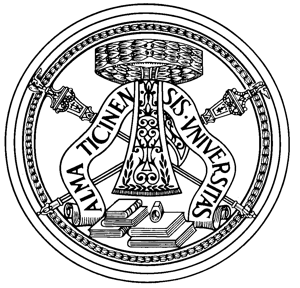
\includegraphics[width=2.5cm]{Figures/Unipv-logo}\\[.5cm] % Institution logo
\LARGE\institution\\ % Print institution name
\Large\emph{\department}\\[.1cm]

\large\course\\[.2cm] % Print department name
\normalsize % Degree or other information
\par
\hrulefill
\vfill}
\renewcommand{\maketitlehookb}{\vfill}

\renewcommand{\maketitlehookc}{
\vfill

\begin{flushleft}
Supervisore:\\
\textbf{Dott. Claudio Dappiaggi}\\[.3cm] % Advisor's/supervisor's name
Co-supervisore:\\
\textbf{Dott. Nicol\'o Drago}\\[.3cm] % Advisor's/supervisor's name
\end{flushleft}
\vfill}
\preauthor{%\LARGE $\Box u=\delta$\\
	\vfill\normalsize\begin{flushright} Relazione per la laurea di:\\\bfseries} % Text prior to the author name - right aligned and bold
\postauthor{\end{flushright}
} % After the author name, stop right alignment

%----------------------------------------------------------------------------------------

\makeindex % Write an index file

\begin{document}

\begin{titlingpage}
\maketitle % Print the title page
\end{titlingpage}

\thispagestyle{empty}

\bigskip\begin{quotation}\begin{center}\begin{em}
			
			\hfill A mamma e pap\`{a}
			
		\par\end{em}\end{center}\end{quotation}

\cleartoverso % Force a break to an even page


\thispagestyle{empty}
\begin{abstract}
	\noindent La tesi si propone di analizzare la risolubilit\'a di equazioni differenziali alle derivate parziali di tipo ondulatorio e le loro propriet\'a tramite la costruzione di soluzioni fondamentali distribuzionali. Dapprima si affronter\'a il caso nello spazio di Minkowski $n$-dimensionale e poi si trasporteranno, per quanto possibile, le principali propriet\'a delle soluzioni su particolari variet\'a curve di interesse per le loro applicazioni fisiche.\\

	\hfill
	
	\noindent The aim of the thesis is to analyse the solvability of wave-like partial differential equations and their properties via the construction of distributional fundamental solutions. Initially will be explored the $n$-dimensional Minkowski case and then the main properties of the solutions will be translated, when possible, on particular manifolds, interesting for their physical applications.
\end{abstract}

\cleartoverso % Force a break to an even page

\frontmatter % Use roman page numbering style (i, ii, iii, iv...) for the pre-content pages
%----------------------------------------------------------------------------------------
%	PREFACE
%----------------------------------------------------------------------------------------

%\section*{Introduzione}
%\textbf{To do}
%\begin{flushright}
%\textsc{\theauthor}\\
%Pavia\\
%July 2017
%\end{flushright}

%\cleartoverso % Force a break to an even page

%------------------------------------------------------------------------------



%----------------------------------------------------------------------------------------
%	TABLE OF CONTENTS
%----------------------------------------------------------------------------------------

\tableofcontents* % Print the table of contents

\cleartoverso % Force a break to an even page


%----------------------------------------------------------------------------------------
%	CONTENT CHAPTERS
%----------------------------------------------------------------------------------------

\mainmatter % Begin numeric (1,2,3...) page numbering

\pagestyle{Ruled} % Include the chapter/section in the header along with a horizontal rule underneath

\chapterstyle{thesis2}
\chapter{Introduction}
\label{introduction}

\textit{Backflow} is an exotic quantum-mechanical phenomenon which can be heuristically depicted as a probability current associated to the quantum mechanical description of a particle moving on a line, flowing in the opposite direction with respect to the underlying momentum\footnote{see [\citealp[Abstract]{gand}]}.\\
In detail, we consider non-relativistic particles moving on a straight line. In \textit{quantum mechanics}, we describe the state of this particles at a given instant of time with a \textit{wave-function} $\psi\in L^2(\mR;\mC)$ where $|\psi(x)|^2$ represents the probability density of finding the particle in any open subset $I\subseteq\mR$. The time-evolution of such wave-functions $\psi(t)$ is ruled by the \textit{Schr\"{o}dinger equation}
\begin{equation}
	i\partial_t\psi(t)=H\psi(t)\, ,
\end{equation}
where $H$ is the \textit{Hamiltonian} which codifies the dynamics of the system. Here, for simplicity, we set all parameters and physical constants to $1$. Furthermore, we restrict ourselves to considering particles "travelling to the right". This statement can be formulated by requiring that the Fourier transform of this wave-function in \textit{momentum space} is supported only on $(0,+\infty)$. These wave-functions will be called \textit{right-movers}.\\
In this scenario, one might think that the probability density must flow to the right for all $t\in(0,+\infty)$ and everywhere in space. Hence the probability of finding the particle on the right of a given reference point might seem to be increasing with time. Counterintuitively, instead the probability can decrease in time. this phenomenon is referred to as \textit{quantum backflow}.\\
The scope of this work is to report and to discuss the main results regarding the fundamental properties as well as the magnitude of backflow in two different scenarios: the \textit{non-interacting} and the \textit{interacting} one.\\
For \textit{free particles}, we will prove that the amount of probability which can 
"flow back" through a reference point in a given interval of time is ruled by a suitable bounded and self-adjoint  $B$, called \textit{backflow operator}. Then, we will prove that the maximum amount of backflow $\lambda$ is equal to the supremum of the spectrum of $B$. We refer to $\lambda$ as \textit{backflow constant}. Using numerical methods, we will estimate $\lambda\approx0.038452$. We will also study the spatial extension of backflow using the density current $j_\psi(x)=i/2(\psi(x)\partial_x\psi^*(x)-\psi^*(x)\partial_x\psi(x))$. In detail, we will prove that there exists a constant $\beta_0(f)$ such that
\begin{equation}
	\int_{-\infty}^{\infty}\nspace f(x)j_\psi(x)\, \dd x \ge \beta_0(f)>-\infty
	\label{eq:first}
\end{equation}
for all normalized right-moving wave functions and for all positive averaging functions $f\ge0$.\\
In the \textit{interacting scenario}, we will investigate the presence of backflow for particles scattering against a potential wall $V$. Herein, complications arise since the presence of a potential $V$ implies the splitting of the incident wave-function into a transmitted and a reflected component which travel in opposite direction. This makes the concept of "right-moving" particle less clear. Hence we will introduce \textit{asymptotic} right-movers as those wave-functions that far away in the past, and far away from the potential wall $V$, behave like free and right-moving wave-functions. If we consider a non-interacting right-mover $\phi$, it might be seen as the incoming asymptotic form of an interacting state $\psi$. The link between the two wave-functions is given by the \textit{M\o{}ller operator} $\Omega_V$ of the Hamiltonian with the potential $V$, $\psi=\Omega_V\phi$. In this scattering scenario, our scope is to generalize the result (\ref{eq:first}). Stated differently, we shall study the existence of lower bounds for the average
\begin{equation}
	\int_{-\infty}^{\infty}\nspace\!f(x)j_{\Omega_V\psi}(x)\,\dd x
\end{equation}
for a generic normalized right-mover $\psi$ and for a positive function $f\ge0$. Although the reflection component can interfere, we will prove that there exists, for all short range potentials $V$ and for all positive smearing functions $f\ge0$, a constant $\beta_V(f)>-\infty$ such that
\begin{equation}
	\int_{-\infty}^{\infty}\nspace\!f(x)j_{\Omega_V\psi}(x)\,\dd x\ge\beta_V(f)
	\label{eq:second}
\end{equation}
for all normalized right-mover $\psi$.\\
 \\ 

The thesis is organized as follows.\\
In the first chapter, it will be presented an overview of the main mathematical
notions needed in order to set the discussion on quantum mechanics and backflow. The main
topics will be \textit{Hilbert spaces}, \textit{operators} and their \textit{spectrum}, \textit{Schwartz test-functions}, \textit{Fourier transform} as well as the basic concepts of quantum mechanics with particular attention both to the \textit{interacting picture} in scattering scenarios and to \textit{M\o{}ller operators}. \\
In the second chapter, it will be discussed the backflow effect in a non-interacting scenario. First of all, we will begin with an historical overview of the results obtained in the past concerning quantum backflow, from the first theoretical formulations, until the most recent analytical and numerical results. Then we introduce the problem of backflow for a free-particle. We will define rigorously the concept of \textit{right-mover} and give some examples of wave-functions in which backflow occurs. Then, we will search a lower bound for the flux of probability across a reference point in a given time interval. To do this, we must reformulate the problem as the search for an supremum of the spectrum of an operator called \textit{backflow operator}. We will prove that such a lower bound exists and hence that the flux of probability across the reference point is always greater than $-\lambda$, where $\lambda\in(0,1)$ is the \textit{backflow constant}. At the end of the chapter, numerical methods will be presented in order to estimate $\lambda$. In particular, using the \textit{power method} we will evaluate the backflow constant $\lambda\approx0.038452$.\\
The third chapter is divided in two main sections. In the first one, we will discuss the spatial extension of backflow for normalized right-movers at a given instant of time. It will be proved that the average of the density current for a right-moving state, as in (\ref{eq:first}), is bounded from below by a constant $\beta_0(f)\in(-\infty,0)$. The second section will be devoted to the analysis of backflow in scattering theory. First, the problem of backflow will be reformulated introducing the concept of \textit{asymptotic} right-moving wave-functions. Then, we will study the existence of a negative lower bound for the average current, as in (\ref{eq:second}). To do so, the infimum of the spectrum of an unbounded operator, called \textit{asymptotic current operator} will be investigated. At the end, we will prove that backflow can occur also in scattering scenarios and that the average current is always bigger than a suitable constant $\beta_V(f)$ determined by the potential $V$ and the positive smearing functions $f\ge0$. 
 % Include the introduction chapter

\chapterstyle{thesis} % Change the style of the Chapter header to that defined in structure.tex




% Chapter 1

\chapter{Geometric preliminaries} % Main chapter title

\label{Chapter1} % For referencing the chapter elsewhere, use \ref{Chapter1}


In this chapter, we begin by recalling the basic definitions in order to fix the geometric setting in which we will work.\\
Globally hyperbolic spacetimes $(M,g)$ are used in context of geometric analysis and mathematical relativity because in them there exists a smooth and spacelike Cauchy hypersurface $\Sigma$ and that ensures the well-posedness of the Cauchy problem. Moreover, as shown by Bernal and Sánchez \cite[Th. 1.1]{Bernal-Sanchez-05}, in such spacetimes there exists a splitting for the full spacetime $M$ as an orthogonal product $\mathbb{R}\times\Sigma$. %, where the metric decomposes as $g=-\Lambda \mathrm{d}t^2+g_t$, where $\Lambda$ is a smooth positive function.
These results corroborate the idea that in globally hyperbolic spacetimes one can preserve the notion of a global passing of time. In a globally hyperbolic spacetime, the entire future and past history of the universe can be predicted from conditions imposed at a fixed instant represented by the hypersurface $\Sigma$.\\
%Standard globally hyperbolic spacetimes can otherwise be defined as the strongly causal spacetimes\footnote{$M$ satisfies the strong causality condition if there are no almost closed causal curves, i.e. if for any	$p \in M$ there exists a neighborhood $U$ of $p$ such that there exists no timelike curve that passes through $U$ more than once.} whose intrinsic causal boundary points are not naked singularities.\\
%
%In a natural way, the timelike boundary $\partial M$ of our class of spacetimes is composed by all
%the naked singularities so, these singularities become the natural
%place to impose boundary conditions.

\section{Globally Hyperbolic spacetimes with timelike boundary}
The main goal of this section is to analyse the main properties of globally hyperbolic spacetimes and to generalise them to a natural class of spacetimes where boundary values problems can be formulated. This class is that of globally hyperbolic spacetimes with timelike boundary.While, in the case of $\partial M=\emptyset$ global hyperbolicity is a standard concept, in presence of a timelike boundary it has been properly defined and studied recently in \cite{Ake-Flores-Sanchez-18}.\\

\noindent\textbf{Manifolds with boundary.} From now on $M$ will denote a smooth manifold with boundary with dimension $m>1$. $M$ is then locally diffeomorphic to open subsets of the closed half space of $\mathbb{R}^n$. We will assume that the boundary $\partial M$ is smooth and, for simplicity, connected. A point $p\in M$ such that there exists an open neighbourhood $U$ containing $p$, diffeomorphic to an open subset of $\mathbb{R}^m$, is called an {\em interior point} and the collection of these points is indicated with $\operatorname{Int}(M)\equiv\mathring{M}$. As a consequence $\partial M\doteq M\setminus\mathring{M}$, if non empty, can be read as an embedded submanifold $(\partial M,\iota_{\partial M})$ of dimension $n-1$ with $\iota_{\partial M}\in C^\infty(\partial M; M)$.\\
In addition we endow $M$ with a smooth Lorentzian metric $g$ of signature $(-,+,...,+)$ so that $\iota^*g$ identifies a Lorentzian metric on $\partial M$ and we require $(M,g)$ to be time oriented. As a consequence $(\partial M,\iota^*_{\partial M}g)$ acquires the induced time orientation and we say that $(M,g)$ has a {\em timelike boundary}. 

\begin{Definition}\label{Def: spacetime timelike boundary}\hfill\\
	\vspace{-0.6cm}
	\begin{itemize}
	\item A spacetime with timelike boundary is a time-oriented Lorentzian manifold with timelike boundary.
	\item A spacetime with timelike boundary is {\em causal} if it possesses no closed, causal curve,
	\item A causal spacetime with timelike boundary $M$ such that for all $p,q\in M$ $J_+(p)\cap J_-(q)$ is compact is called \textbf{globally hyperbolic}.
	\end{itemize}
\end{Definition}

These conditions entail the following consequences, see \cite[Th. 1.1 \& 3.14]{Ake-Flores-Sanchez-18}:

\begin{theorem}
	Let $(M,g)$ be a spacetime of dimension $m$. Then 
	\begin{enumerate}
		\item $(M,g)$ is a globally hyperbolic spacetime with timelike boundary if and only if it possesses a Cauchy surface, namely an achronal subset of $M$ which is intersected only once by every inextensible timelike curve,
		\item if $(M,g)$ is globally hyperbolic, then it is isometric to $\mathbb{R}\times\Sigma$ endowed with the metric
		\begin{equation}\label{eq:line_element}
		g=-\beta d\tau^2+h_\tau,
		\end{equation}
		where $\tau:M\to\mathbb{R}$ is a Cauchy temporal function\footnote{Given a generic time oriented Lorentzian manifold $(N,\tilde{g})$, a Cauchy temporal function is a map $\tau:M\to\mathbb{R}$ such that its gradient is timelike and past-directed, while its level surfaces are Cauchy hypersurfaces.}, whose gradient is tangent to $\partial M$, $\beta\in C^\infty(\mathbb{R}\times\Sigma;(0,\infty))$ while $\mathbb{R}\ni\tau\to (\{\tau\}\times\Sigma,h_\tau)$ identifies a one-parameter family of $(n-1)-$dimensional spacelike, Riemannian manifolds with boundaries. Each $\{\tau\}\times\Sigma$ is a Cauchy surface for $(M,g)$.
	\end{enumerate}
\end{theorem}


Henceforth we will be tacitly assuming that, when referring to a globally hyperbolic spacetime with timelike boundary $(M,g)$, we work directly with \eqref{eq:line_element} and we shall refer to $\tau$ as the time coordinate. Furthermore each Cauchy surface $\Sigma_\tau\doteq\{\tau\}\times\Sigma$ acquires an orientation induced from that of $M$.

\begin{Definition}
	A spacetime $(M,g)$ is {\em static} if it possesses a timelike Killing vector field $\chi\in\Gamma(TM)$ whose restriction to $\partial M$ is tangent to the boundary, {\it i.e.} $g_p(\chi,\nu)=0$ for all $p\in\partial M$ where $\nu$ is the unit vector, normal to the boundary at $p$.
\end{Definition}
With reference to \eqref{eq:line_element} this translates simply into the request that both $\beta$ and $h_\tau$ are independent from $\tau$.

\begin{Example}
	We first consider some examples of globally hyperbolic spacetimes without boundary ($\partial M=\emptyset$).
	\begin{itemize}
		\item The Minkowski spacetime $M=(\mathbb{R}^m,\eta)$ is stati and globally hyperbolic. Every spacelike hyperplane is a Cauchy hypersurface. We have $M=\mathbb{R}\times \Sigma$ with $\Sigma = \mathbb{R}^{m-1}$, endowed with the time-independent Euclidean metric.
		\item Let $\Sigma$ be a Riemannian manifold with time independent metric $h$ and $I\subset\mathbb{R}$ an interval. Let $f: I\to\mathbb{R}$	be a smooth positive function. The manifold $M=I \times \Sigma$ with the metric $g = -\mathrm{d} t^2 + f^2(t)\, h$, called \textbf{cosmological spacetime}, is globally hyperbolic if and only if $(\Sigma,h)$ is a complete Riemannian manifold, see \cite[Lem A.5.14]{Baer-Ginoux-Pfaffle-07}. This applies in particular if $(\Sigma,h)$ is compact.
		\item The interior and exterior \textbf{Schwarzschild spacetimes}, that represent non-rotating black holes of mass $\mathrm{m}>0$ are static and globally hyperbolic.
		Denoting $S^2$ the $2$-dimensional sphere embedded in $\mathbb{R}^3$, we set
		\[	 M_{\text{ext}}:=\mathbb{R}\times(2\mathrm{m},+\infty)	\times S^2,	\] 
		
		\[	 M_{\text{int}}:=\mathbb{R}\times(0,2\mathrm{m})	\times S^2.	\] 
		The metric is given by
		\[	g=-f(r) \mathrm{d} t^2+\frac{1}{f(r)} \mathrm{d} r^2	+r^2\,g_{S^2},	\]
		where $f(r)=1-\frac{2\mathrm{m}}{r}$, while $g_{S^2}=r^2\, \mathrm{d}\theta^2+r^2\sin^2\theta \mathrm{d}\varphi^2$ is the polar coordinates metric on the sphere. For the exterior Schwarzschild spacetime we have $ M_{\text{ext}}=\mathbb{R}\times \Sigma$ with $\Sigma=(2\mathrm{m},+\infty)\times S^2$, $\beta=f$ and $h=\frac{1}{f(r)} \mathrm{d} r^2	+r^2\,g_{S^2}$.
	\end{itemize}
\end{Example}

\begin{Example}
	Now we consider some examples of globally hyperbolic spacetimes with timelike boundary in which the boundary is not empty.
	\begin{itemize}
		\item The Half Minkowski spacetime $M=(\mathbb{R}^{m-1}\times[0,+\infty),\eta)$ is static and globally hyperbolic. Every spacelike half-hyperplane is a Cauchy hypersurface. We have $M=\mathbb{R}\times \Sigma$ with $\Sigma= \mathbb{R}^{m-2}\times[0,+\infty)$, endowed with the time-independent Euclidean metric.
		\item Let $\Sigma$ be a Riemannian manifold with boundary with time independent metric $h$ and $I\subset\mathbb{R}$ an interval. Let $f: I\to\mathbb{R}$	be a smooth positive function. The manifold $M=I \times \Sigma$ with the metric $g = -\mathrm{d} t^2 + f^2(t)\, h$ is globally hyperbolic if and only if $(\Sigma,h)$ is a complete Riemannian manifold with boundary.
	\end{itemize}
\end{Example}

 A particular role will be played by the support of the functions that we consider. In the following definition we introduce the different possibilities that we will consider - \textit{cf.} \cite{Baer-15}.
\begin{Definition}\label{Def: space of forms}
	Let $(M,g)$ be a Lorentzian spacetime with timelike boundary. We denote with 
	\begin{enumerate}
		\item 	$ C^\infty_{\mathrm{c}}(M)$ the space of smooth functions with compact support in $M$ while with $ C^\infty_{\mathrm{cc}}(M)\subset C^\infty_{\mathrm{c}}(M)$ the collection of smooth and compactly supported functions $ f$ such that $\textrm{supp}( f)\cap\partial M=\emptyset$.
		\item
		$ C^\infty_{\mathrm{spc}}(M)$ (\textit{resp}. $ C^\infty_{\mathrm{sfc}}(M)$) the space of strictly past compact (\textit{resp.} strictly future compact) functions, that is the collection of $ f\in C^\infty(M)$ such that there exists a compact set $K\subseteq M$ for which $J^+(\textrm{supp}( f))\subseteq J^+(K)$ (\textit{resp.} $J^-(\textrm{supp}( f))\subseteq J^-(K)$), where $J^\pm$ denotes the causal future and the causal past in $M$.  Notice that $ C^\infty_{\mathrm{sfc}}(M)\cap C^\infty_{\mathrm{spc}}(M)= C^\infty_{\mathrm{c}}(M)$.
		\item
		$ C^\infty_{\mathrm{pc}}(M)$ (\textit{resp}. $ C^\infty_{\mathrm{fc}}(M)$) denotes the space of future compact (\textit{resp.} past compact) functions, that is, $ f\in C^\infty(M)$ for which
		${\rm supp}( f)\cap J^-(K)$ (\textit{resp.} ${\rm supp}( f)\cap J^+(K)$) is compact for all compact $K\subset M$.
		\item $ C^\infty_{\mathrm{tc}}(M):= C^\infty_{\mathrm{fc}}(M)\cap C^\infty_{\mathrm{pc}}(M)$, the space of timelike compact functions.
		\item $ C^\infty_{\mathrm{sc}}(M):= C^\infty_{\mathrm{sfc}}(M)\cap C^\infty_{\mathrm{spc}}(M)$, the space of spacelike compact functions.
	\end{enumerate}
\end{Definition}

\section{Differential forms and operators on manifolds with boundary}

To treat Maxwell equations properly and to be able to generalise them, we will use the language of differential forms.
In this section $(E,g)$ will denote a generic oriented pseudo-Riemannian manifold with boundary with signature $(-,+,\dots,+,+)$ or $(+,+,\dots,+,+)$. In the former case, when the manifold is Lorentzian, it is understood that the boundary is timelike in the sense of Definition \ref{Def: spacetime timelike boundary}. We present the following definitions in such a general framework since we will work both on spacetimes $(M,g)$ with timelike boundary and on their Cauchy hypersurfaces $(\Sigma,h)$, which are Riemannian manifolds with boundary.\\



On top of a pseudo-Riemannian Hausdorff, connected, oriented and paracompact manifold $(E,g)$ with boundary we consider the spaces of complex valued $k$-forms $\Omega^k(E)$ as smooth sections of $\wedge^kT^*E$. Since $(E,g)$ is oriented, we can identify a unique, metric-induced, Hodge operator $\ast:\Omega^k(E)\to\Omega^{m-k}(E)$, $m=\dim E$ such that, for all $\alpha,\beta\in\Omega^k(E)$, $\alpha\wedge\ast\beta=(\alpha,\beta)\mathrm{d}\mu_g$, where $\wedge$ is the exterior product of forms and $\mathrm{d}\mu_g$ the metric induced volume form. We endow $\Omega^k(E)$ with the standard, metric induced, pairing
\begin{align}
(\alpha,\beta):=\int_E\overline{\alpha}\wedge\ast\beta\,,
\end{align}


\begin{remark}
	One can easily generalize of the spaces defined for scalar fields in Definition \ref{Def: space of forms} respectively to the following spaces of $k$-forms: $\Omega_\mathrm{c}^k(M)$, $\Omega_{\mathrm{cc}}^k(M)$, $\Omega_{\mathrm{spc}/\mathrm{sfc}}^k(M)$, $\Omega_{\mathrm{pc}/\mathrm{fc}}^k(M)$, $\Omega_{\mathrm{tc}/\mathrm{sc}}^k(M)$.
\end{remark}


We indicate the exterior derivative with $\mathrm{d}:\Omega^k(E)\to\Omega^{k+1}(E)$. A differential form $\alpha$ is called closed when $\mathrm{d}\alpha=0$ and exact when $\alpha=\mathrm{d}\beta$ for some differential form $\beta$. Since $E$ is endowed with a pseudo-Riemannian metric it holds that, when acting on smooth $k$-forms, $\ast^{-1}=(-1)^{k(m-k)}\ast$. Combining these data we define the {\em codifferential} operator $\delta:\Omega^{k+1}(E)\to\Omega^k(E)$ as $\delta\doteq\ast^{-1}\circ \mathrm{d}\circ\ast$.

%
%If the spacetime is static, $M$ can be decomposed as $\mathbb{R}\times\Sigma$, where $(\Sigma, h)$ is an oriented Riemannian Manifold with boundary.
%In this case we distinguish, on $(\Sigma,h)$ for $k\in\mathbb{N}\cup\{0\}$:
%\begin{itemize}
%	\item the space of smooth forms $C^\infty\Omega^k(\Sigma)$,
%	\item the space of compactly supported smooth forms $C^\infty_c\Omega^k(\Sigma)$,
%	\item the space of square integrable forms (with respect to $(\,,\,)\ $) $\mathrm{L}^2\Omega^k(\Sigma)$,
%\end{itemize}
%



%
%Now we define the main operators with which we will deal along the thesis.
%\begin{Definition}
%	We introduce the {\em D'Alembert-de Rham} wave operator $\Box_k:\Omega^k(M)\to\Omega^k(M)$ such that $$\Box_k\doteq \mathrm{d}\delta+\delta \mathrm{d},$$ as well as the {\em Maxwell} operator $\mathcal{M}_k:\Omega^k(M)\to\Omega^k(M)$ such that $$\mathcal{M}_k\doteq\delta \mathrm{d}.$$
%\end{Definition}
%The subscript $k$ is here introduced to make explicit on which space of $k$-forms the operator is acting. Usually, the subscript $k$ is dropped because if there are no boundary conditions the operators act separately on each component of the forms. Observe, furthermore, that $\Box_k$ differs by the more commonly used D'Alembert wave operator acting on $k$-forms by $0$-order term built out of the metric and whose explicit form depends on the value of $k$, see for example \cite[Sec. II]{Pfenning:2009nx}.
%
%The name {\em Maxwell operator} for $\delta\mathrm{d}$ was given in view of Maxwell equations for electromagnetism. Written in terms of the potential $1$-form $A$, they look like
%\begin{equation}\label{Eqn: maxwell}
%	-\mathcal{M}_1A=-\delta\mathrm{d}A=J,
%\end{equation}
%where $J$ is the current $1$-form, which vanishes in vacuum. The higher order Maxwell operators lead to a generalisation of electromagnetism to forms of higher degree, which will be treated along the thesis, letting $k$ be in $\mathbb{N}$.

To conclude the section, we focus on the boundary $\partial E$ and on the interplay with $k$-forms lying in $\Omega^k(E)$. The first step consists of defining two notable maps. These relate $k$-forms defined on the whole $E$ with suitable counterparts living on $\partial E$ and, in the special case of $k=0$, they coincide either with the restriction to the boundary of a scalar function or with that of its projection along the direction normal to $\partial E$.

\begin{remark}
	Since we will be considering not only form lying in $\Omega^k(E)$, $k\in\mathbb{N}\cup\{0\}$, but also those in $\Omega^k(\partial E)$, we shall distinguish the operators acting on this space with a subscript $_\partial$, {\it e.g.} $\mathrm{d}_\partial$, $\ast_\partial$, $\delta_\partial$ or $(,)_\partial$.
\end{remark}



\begin{Definition}\label{Def: tangential and normal component}
	Let $(E,g)$ be a pseudo-Riemannian manifold with boundary together with the embedding map $\iota_{\partial}:\partial E\hookrightarrow E$. We call {\em tangential} and {\em normal} maps 
	\begin{subequations}\label{Eqn: tangential and normal maps}
		\begin{equation}\label{Eqn: tangential map}
		\mathrm{t}\colon\Omega^k(E)\to\Omega^k(\partial E)\qquad\omega\mapsto\mathrm{t}\omega\doteq\iota_{\partial}^*\omega
		\end{equation}
		\begin{equation}\label{Eqn: normal maps}
		\mathrm{n}\colon\Omega^k(E)\to\Omega^{k-1}(\partial E)\qquad\omega\mapsto\mathrm{n}\omega\doteq\ast_{\partial}^{-1}\circ\mathrm{t}\circ\ast_E\,,
		\end{equation}
	\end{subequations}
	In particular, for all $k\in\mathbb{N}\cup\{0\}$ we define
	\begin{align}\label{Eqn: k-forms with vanishing tangential or normal component}
	\Omega_{\mathrm{t}}^k(E):=\lbrace\omega\in\Omega^k(E)\;|\;\mathrm{t}\omega=0\rbrace\,,\qquad
	\Omega_{\mathrm{n}}^k(E):=\lbrace\omega\in\Omega^k(E)\;|\;\mathrm{n}\omega=0\rbrace\,.
	\end{align}
\end{Definition}

\begin{remark}
	The normal map $\mathrm{n}:\Omega^k(E)\to\Omega^{k-1}(\partial E)$ can be equivalently read as the restriction to $\partial E$ of the contraction $\nu\operatorname{\lrcorner}\omega$ between $\omega\in\Omega^k(E)$ and the vector field $\nu\in\Gamma(TE)|_{\partial E}$ which corresponds pointwisely to the unit vector, normal to $\partial E$.
\end{remark}

\noindent As last step, we observe that \eqref{Eqn: tangential and normal maps} together with \eqref{Eqn: k-forms with vanishing tangential or normal component} entail the following series of identities on $\Omega^k(E)$ for all $k\in\mathbb{N}\cup\{0\}$.
\begin{subequations}\label{Eqn: relations between d,delta,t,n}
	\begin{equation}\label{Eqn: relations-bulk}
	\ast\delta=(-1)^k\mathrm{d}\ast\,,\quad
	\delta\ast=(-1)^{k+1}\ast\mathrm{d}\,,
	\end{equation}
	\begin{equation}\label{Eqn: relations-bulk-to-boundary}
	\ast_\partial\mathrm{n}=\mathrm{t}\ast\,,\quad
	\ast_\partial\mathrm{t}=(-1)^k\mathrm{n}\ast\,,\quad
	\mathrm{d}_\partial\mathrm{t}=\mathrm{t}\mathrm{d}\,,\quad
	\delta_\partial\mathrm{n}=\mathrm{n}\delta\,.
	\end{equation}
\end{subequations}
A notable consequence of \eqref{Eqn: relations-bulk-to-boundary} is that, while on manifolds with empty boundary, the operators $\mathrm{d}$ and $\delta$ are one the formal adjoint of the other, in the case in hand, the situation is different. Indeed, a direct application of Stokes' theorem yields that 
\begin{align}\label{Eqn: boundary terms for delta and d}
(\mathrm{d}\alpha,\beta)-(\alpha,\delta\beta)=
(\mathrm{t}\alpha,\mathrm{n}\beta)_\partial\qquad
\forall\alpha\in\Omega_{\mathrm{c}}^k(E)\,,\;
\forall\beta\in\Omega_{\mathrm{c}}^{k+1}(E)\,,
\end{align}
where the pairing in the right-hand side is the one associated to forms living on $\partial E$.

\section{Maxwell equations for $k$-forms}\label{Sec: Maxwell introduction}
We now focus our attention on a $m$-dimensional spacetime $(M,g)$.
As usual, the electromagnetic field will be regarded as a $2$-form $F$, called Faraday field, and the potential as a $1$-form $A$ such that, locally, holds $F=\mathrm{d}A$. This is permitted by the first Maxwell equation, namely
\begin{equation}\label{Eqn: first maxwell}
	\mathrm{d}F=0,
\end{equation}
that ensures the Faraday form $F$ being closed, hence locally exact. The equation $F=\mathrm{d}A$ holds globally whenever one can rely on the Poincaré lemma, which cannot be always applied since it fails to hold true if the second cohomology group $H^2 (M )$ is not trivial.\\

From a physical point of view, one wonders whether it is $A$ or it is $F$ the observable field of the dynamical system, because $F$ encodes the usual electric and magnetic fields $E,B\in\Omega^1(\Sigma)$ (if $M$ is static with $M=\mathbb{R}\times\Sigma$, holds the decomposition $F=\ast_{\Sigma}B+\mathrm{d}t\wedge E$). Moreover, one can object that the choice of $A\in\Omega^{1}(M)$ is not unique. Indeed if for a moment one assumes, for simplicity, $M$ to be globally hyperbolic with empty boundary, the configuration $A':=A+\mathrm{d}\chi$, $\chi\in\Omega^0(M)$ is equivalent to $A$ since it gives rise to the same Faraday field $F$. This freedom in the choice of $A$ is extensively used and it is called \textbf{gauge freedom}.\\

To recap, one can regard the electromagnetism as a theory for $F\in\Omega^2(M)$ or as a theory for a non-unique $A\in\Omega^1(M)$ and wonder if the initial and boundary value problem for Maxwell equations is well-posed in both cases. The former case for $F$ will be covered in Chapter \ref{Chapter2} and the latter for $A$ in Chapter \ref{Chapter3}.\\

The second Maxwell equations tells us the dynamics of the electromagnetic field. If $J$ denotes the co-closed current $1$-form ($\delta J=0$), which encodes the charge density and the electric current, the second Maxwell equation can be written as
\begin{equation}\label{Eqn: second maxwell}
	\delta F=-J,
\end{equation}
and the corresponding

In the homogeneous case ($J=0$), one can generalise the Maxwell field to be $F\in\Omega^k(M)$, imposing $\mathrm{d}F=0$ and $\delta F=0$ and the equation for $A\in\Omega^{k-1}(M)$ becomes $\delta\mathrm{d}A=0$. In this case gauge freedom is understood as a transformation $A\mapsto A+\mathrm{d}\chi$, $\chi\in\Omega^{k-2}(M)$.

 % Include the first content chapter
\chapter{Maxwell equations with interface conditions} % Main chapter title

\label{Chapter2} % For referencing the chapter elsewhere, use \ref{Chapter1}



%Section \ref{Sec: Maxwell equations with interface conditions} deals with the construction of the algebra of observable associated with the Faraday tensor $F$ in the presence of an interface $Z$.
%For that we need Hodge decomposition, boundary triples out of which we define an exact sequence -- \textit{cf.} proposition \ref{Prop: exact sequence for Maxwell equations with interface}.

As outlined in Section \ref{Sec: Maxwell introduction}, the very nature of Maxwell equations allows us to use both $F$ and $A$ as variables with which to describe electromagnetic phenomena. Whenever the second cohomology group $H^2(M)$ is trivial, the two theories are equivalent, since $F=\mathrm{d}A$.


In this chapter, we regard $F\in\Omega^2(M)$ as the true physical dynamical variable which describes electromagnetism. The aim of this chapter is to present a technique which allows to characterize, in a class of manifolds with the presence of an interface between two media, the existence of fundamental solutions for Maxwell equations, written in terms of the Faraday form $F\in\Omega^2(M)$. The presence of an interface on the one hand generalizes the idea of the presence of a timelike boundary, allowing to recover the geometric setting outlined in Chapter \ref{Chapter1} in case on one side of the interface lies a perfect insulator. On the other hand, in order to make use of geometric techniques such as Hodge decomposition, we will have to make several geometric assumptions which ensure global hyperbolicity, but unfortunately are way less general.

\section{Geometrical set-up}
The physical and practical situation we want to approach is that of a manifold split into two parts, filled with two media, each of them with different electromagnetic properties. The two media will be separated by an hypersurface, on which our aim will be that of putting \emph{jump conditions}.

We consider a static Lorentzian manifold $(M,g)$ with \textbf{empty boundary}, such that $M$ can be decomposed as $\mathbb{R}\times\Sigma$, where the Cauchy hypersurface $(\Sigma,h)$ is assumed to be a complete, connected, odd-dimensional, \textbf{closed} Riemannian manifold.
%\\\nicomment{(We should look for references where the (weak) Hodge decomposition is established for non-compact Riemannian manifold with boundary. If this is the case and if the results presented below remain valid with the weak Hodge decomposition, we will drop the closedness assumption.)}\\
The assumptions we made so far on imply that $(M,g)$ is a globally hyperbolic spacetime without boundary.

Maxwell equations, recalling formulas \eqref{Eqn: first maxwell} and \eqref{Eqn: second maxwell}, for $F\in\Omega^2(M)$ are simply
\begin{align}\label{Eqn: covariant Maxwell equations}
\mathrm{d}F=0\,,\qquad\delta F=0\,,
\end{align}
The geometrical assumptions on $M$ permit us to split $F$ into electric and magnetic components
\begin{align}\label{Eqn: electric and magnetic components}
F=\ast_\Sigma B+\mathrm{d}t\wedge E\,,
\end{align}
where $E,B\in\Omega^1(\Sigma)$ while $\ast_\Sigma$ is the Hodge dual of $\Sigma$.\\
Maxwell equations are then reduced to
\begin{subequations}\label{Eqn: Maxwell equations}
	\begin{align}
	\label{Eqn: dynamical Maxwell equations}
	\partial_tE-\mathrm{curl}B=0\,,\qquad
	\partial_tB+\mathrm{curl}E=0\,,\\
	\label{Eqn: non-dynamical Maxwell equations}
	\mathrm{div}(E)=\mathrm{div}(B)=0\,,
	\end{align}
\end{subequations}
where $\mathrm{div}=\delta_\Sigma$ is the co-differential of $\Sigma$, while $\mathrm{curl}$ is defined in equation \eqref{Eqn: curl convention} -- in particular $\mathrm{curl}=\ast_\Sigma\mathrm{d}_\Sigma$ if $\dim\Sigma=3\mod 4$.\\
To model the presence of an interface that divides $M$ in two distinct regions, we also let $Z$ be a codimension $1$ smooth embedded hypersurface of $\Sigma$.

We denote with $\mathrm{d},\delta$ the differential and co-differential over $M$, while $\mathrm{d}_\Sigma,\delta_\Sigma$ denote the differential and co-differential over $\Sigma$.

In this setting we would like to consider Maxwell equations with $Z$-interface boundary conditions. This means that we will consider Maxwell equations on $M\setminus(\mathbb{R}\times Z)$, allowing for jump discontinuities to occur on $\mathbb{R}\times Z$.
\\\nicomment{(We should decide whether we want to consider $k$-Maxwell equations or not.
	In the former case the $\mathrm{curl}$ operator acts as $\mathrm{curl}\colon\Omega^k(\Sigma)\to\Omega^k(\Sigma)$ where $\dim\Sigma=2k+1$.)}\\


Whenever $Z\neq\emptyset$ the system \eqref{Eqn: Maxwell equations} has to be modified, in particular the non-dynamical equations \eqref{Eqn: non-dynamical Maxwell equations} involving the divergence operator $\mathrm{div}$ have to be suitably interpreted -- \textit{cf.} remark \ref{Rmk: Hodge formulation of non-dynamical Maxwell equations}.
In particular one expects that the condition $\operatorname{div}(E)=\mathrm{div}(B)=0$ should be interpreted weakly, leading to a constraint on the normal jump of $E$ across $Z$.
Moreover, the dynamical equations \eqref{Eqn: dynamical Maxwell equations} have to be combined with boundary conditions at the interface $Z$ -- \textit{cf.} \cite[Sec. I.5]{Jackson-99}.

In what follows we will state the precise meaning of the problem \eqref{Eqn: Maxwell equations} with interface $Z$ with the help of Hodge theory and Lagrangian subspaces \cite{Everitt-Markus-99,Everitt-Markus-03,Everitt-Markus-05}.
%boundary triples theory \cite{Behrndt-Langer-12}.


\section{Non-dynamical equations: Hodge theory with interface}\label{Sec: Non-dynamical equations: Hodge theory with interface}
In this section we present a Hodge decomposition for the closed Riemannian manifold $(\Sigma,h)$ with interface $Z$.
This generalizes the known results on classical Hodge decomposition on manifolds with possible non-empty boundary \cite{Amar-17,Axelsson-McIntosh-04,Gaffney-55,Gromov-91,Kodaira-49,Li-09,Schwarz-95,Scott-95,Zulfikar-Stroock-00}.\\



Hodge theory comes as a generalization of Helmholtz decomposition. He first formulated a result on the splitting of vector fields into vortices and gradients, which can be understood as a rudimentary form of what is now called the \emph{Hodge decomposition}. The idea behind Helmholtz decomposition is that any vector field in $\mathbb{R}^3$ can be decomposed as a sum of an irrotational field, i.e. $\operatorname{curl}=\mathrm{d}_\Sigma=0$, and a solenoidal field, i.e. $\operatorname{div}=\delta_\Sigma=0$. In other words, for $\mathbf{F}\in C^2(\mathbb{R}^3,\mathbb{R}^3)$, one can write
\begin{equation}
\mathbf{F}=-\nabla\Phi+\operatorname{curl}\mathbf{A}.
\end{equation}


In what follows $\mathrm{L}^2\Omega^k(\Sigma)$ will denote the space of sections of $\wedge^kT^*\Sigma$ which are square integrable with respect to the pairing induced by the metric $h$
\begin{align}\label{Eqn: L2-scalar product}
	(\alpha,\beta)_\Sigma:=\int_\Sigma\overline{\alpha}\wedge\ast_\Sigma\beta\,,
\end{align}
where $\ast_\Sigma$ is the Hodge dual.
Similarly we shall denote with $C^\infty_{\mathrm{c}}\Omega^k(\Sigma)$ the space of smooth and compactly supported $k$-forms, while $\mathrm{H}^\ell\Omega^k(\Sigma)$ will denote $k$-forms with weak $\mathrm{L}^2$-derivatives up to order $\ell\in\mathbb{N}\cup\{0\}$ with respect to one (hence all) connection over $\Sigma$ -- as usual we also set $\mathrm{H}^{-\ell}\Omega^k(\Sigma):=\mathrm{H}^\ell\Omega^k(\Sigma)^*$.
\\\nicomment{(If $\Sigma$ is not compact we only have that only $\mathrm{H}^\ell_{\mathrm{loc}}(\Sigma)$ is independent from the choice of the connection.
	If we assume $(\Sigma,h)$ to be of bounded geometry the ambiguity disappears because of the results of \cite{Eichorn-93}.)}\\

\subsection{Hodge decomposition on compact manifold with non-empty boundary}
The Hodge theorem for a closed manifold $\Sigma$ states that there is an $\mathrm{L}^2$-orthogonal decomposition
\begin{align}\label{Eqn: Hodge decomposition on closed manifolds}
	\mathrm{L}^2\Omega^k(\Sigma)=\mathrm{d}_\Sigma \mathrm{H}^1\Omega^{k-1}(\Sigma)\oplus\delta_\Sigma \mathrm{H}^1\Omega^{k+1}(\Sigma)\oplus\ker(\Delta)_{\mathrm{H}^1\Omega^k(\Sigma)}\,,
\end{align}
where $\Delta=\mathrm{d}_\Sigma\delta_\Sigma+\delta_\Sigma\mathrm{d}_\Sigma$ is the Laplacian and $\ker(\Delta)_{\mathrm{H}^1\Omega^k(\Sigma)}$ denotes the space of \emph{harmonic forms}.
If $\Sigma$ has no an empty boundary, the space of harmonic forms $\ker(\Delta)_{\mathrm{H}^1\Omega^k(\Sigma)}$ coincides with that of \textbf{harmonic fields}, defined (following \cite{Kodaira-49} and \cite{Schwarz-95}) as
\begin{equation}\label{Eqn: harmonic fields}
	\mathcal{H}^k(\Sigma)=\lbrace\omega\in \mathrm{H}^1\Omega^k(\Sigma)|\;\mathrm{d}_\Sigma\omega=0\,,\;\delta_\Sigma\omega=0\rbrace=\ker(\delta_\Sigma)_{\mathrm{H}^1\Omega^k(\Sigma)}\cap\ker(\mathrm{d}_\Sigma)_{\mathrm{H}^1\Omega^k(\Sigma)}\,.
\end{equation}
The last result can be stated as follows and it is very easy to prove.
\begin{proposition}
	Let $\alpha\in\mathrm{H}^1\Omega^k(\Sigma)$, where $\Sigma$ is a closed manifold. Then $\Delta\alpha=0$ if and only if $\mathrm{d}_\Sigma\alpha=0$ and $\delta_\Sigma\alpha=0$.
\end{proposition}
\begin{proof}
	Clearly if $\mathrm{d}_\Sigma\alpha=0$ and $\delta_\Sigma\alpha=0$, $\Delta\alpha=0$. On the other hand if $\Delta\alpha=0$,
	\begin{align}
		0=&\left(\Delta\alpha,\alpha\right)_\Sigma=\left((\mathrm{d}_\Sigma\delta_\Sigma+\delta_\Sigma\mathrm{d}_\Sigma)\alpha,\alpha\right)_\Sigma=\left(\mathrm{d}_\Sigma\delta_\Sigma\alpha,\alpha\right)_\Sigma+\left(\delta_\Sigma\mathrm{d}_\Sigma\alpha,\alpha\right)_\Sigma=\\
		=&\left(\delta_\Sigma\alpha,\delta_\Sigma\alpha\right)_\Sigma+\left(\mathrm{d}_\Sigma\alpha,\mathrm{d}_\Sigma\alpha\right)_\Sigma=||\delta_\Sigma\alpha||^2+||\mathrm{d}_\Sigma\alpha||^2.
	\end{align}
	So both $\mathrm{d}_\Sigma\alpha=0$ and $\delta_\Sigma\alpha=0$.
\end{proof}
For a compact manifold $\Sigma$ with non-empty boundary $\partial\Sigma$ the decomposition \eqref{Eqn: Hodge decomposition on closed manifolds} requires a slight adjustment and harmonic forms do not coincide with harmonic fields anymore.
Because of boundary terms, $\ker\Delta$ no longer coincides with the closed and co-closed forms. It is clear that every harmonic field is a harmonic form, but the converse is false. To show this, consider the following example.
\begin{Example}
	Let $U$ a bounded subset of $\mathbb{R}^2$, endowed with the standard euclidean metric. On $U$, the 1-form $\omega=x \,dy$ is clearly harmonic, since its second derivatives vanish, but it is not in $\ker \mathrm{d}$ as
	
	\[\mathrm{d}(x\, \mathrm{d}y) = \partial_x\, x\, \mathrm{d}x \wedge \mathrm{d}y + \partial_y\, x\, \mathrm{d}y \wedge \mathrm{d}y = \mathrm{d}x \wedge \mathrm{d}y.\] $\omega$ is though in $\ker \delta$ as $\ast \mathrm{d} \ast (x\, \mathrm{d}y) =\ast \mathrm{d}(x \,\mathrm{d}x) = 0$.
\end{Example}


In fact, the space $\mathcal{H}^k(\Sigma)$ of harmonic fields is infinite dimensional and so is much too big to represent the cohomology, and to recover the Hodge isomorphism one has to impose boundary conditions. Indeed the spaces $\mathrm{d}_\Sigma \mathrm{H}^1\Omega^{k-1}(\Sigma)$, $\delta_\Sigma H^{1}\Omega^{k+1}(\Sigma)$, $\mathcal{H}^k(\Sigma)$ are not orthogonal unless suitable boundary conditions are imposed.

\begin{remark}\label{Rmk: extension of tangential and normal maps to Sobolev spaces}
	According to \cite[p. 171]{Georgescu-79}, the tangential and normal maps defined in Definition \ref{Def: tangential and normal component} can be extended to continuous surjective maps
	\begin{align}\label{Eqn: Sobolev tangential and normal trace maps}
		\mathrm{t}\oplus\mathrm{n}\colon
		\mathrm{H}^\ell\Omega^k(\Sigma)\to
		\mathrm{H}^{\ell-\frac{1}{2}}\Omega^k(\partial\Sigma)\oplus
		\mathrm{H}^{\ell-\frac{1}{2}}\Omega^k(\partial\Sigma)\,\qquad\forall\ell\geq\frac{1}{2}\,.
	\end{align}
\end{remark}
We can now recall the Hodge decomposition for compact manifolds with boundary \cite[Thm. 2.4.2]{Schwarz-95}.
\begin{theorem}\label{Thm: Hodge decomposition for manifolds with boundary}
	Let $(\Sigma,h)$ be a compact, connected, Riemannian manifold with non-empty boundary $\partial\Sigma\stackrel{\iota_{\partial\Sigma}}{\hookrightarrow}\Sigma$.
	\begin{enumerate}
		\item
		For all $\omega\in C^{\infty}_{\mathrm{c}}\Omega^{k-1}(\Sigma)$ and $\eta\in C^{\infty}_{\mathrm{c}}\Omega^{k}(\Sigma)$ it holds
		\begin{align}\label{Eqn: boundary terms}
			(\mathrm{d}_\Sigma\omega,\eta)_\Sigma-(\omega,\delta_\Sigma\eta)_\Sigma=
			(\mathrm{t}\omega,\mathrm{n}\eta)_{\partial\Sigma}\,,
%			\int_{\partial\Sigma}\mathrm{t}\overline{\omega}\wedge\ast_{\Sigma}\mathrm{n}\eta\,,
		\end{align}
		where $(\;,\;)_\Sigma$ has been defined in equation \eqref{Eqn: L2-scalar product} while $(\;,\;)_{\partial\Sigma}$ is defined similarly.
		Equation \eqref{Eqn: boundary terms} still holds true for $\omega\in \mathrm{H}^\ell\Omega^{k-1}(\Sigma)$ and $\eta\in \mathrm{H}^\ell\Omega^{k}(\Sigma)$ -- \textit{cf.} remark \ref{Rmk: extension of tangential and normal maps to Sobolev spaces}.
		\item
		There is an orthogonal decomposition
		\begin{align}\label{Eqn: Hodge decomposition for manifold with boundary}
			\mathrm{L}^2\Omega^k(\Sigma)=
			\mathrm{d}_\Sigma \mathrm{H}^1\Omega^k_{\mathrm{t}}(\Sigma)\oplus
			\delta_\Sigma \mathrm{H}^1\Omega^{k+1}_{\mathrm{n}}(\Sigma)
			\oplus\mathrm{L}^2\mathcal{H}^k(\Sigma)\,,		
		\end{align}
		where $\mathrm{L}^2\mathcal{H}^k(\Sigma)$ is the closure with respect to the $\mathrm{L}^2$ norm of the space of harmonic fields, as defined per equation \eqref{Eqn: harmonic fields} and
		\begin{align}\label{Eqn: Dirichlet and Neumann forms}
			\mathrm{H}^1\Omega^{k-1}_{\mathrm{t}}(\Sigma):=\lbrace\alpha\in \mathrm{H}^1\Omega^{k-1}(\Sigma)|\;\mathrm{t}\alpha=0\rbrace\,,\\
			\mathrm{H}^1\Omega^{k+1}_{\mathrm{n}}(\Sigma):=\lbrace\beta\in \mathrm{H}^1\Omega^{k+1}(\Sigma)|\;\mathrm{n}\beta=0\rbrace\,,
		\end{align}
	following the definitions of Equation \eqref{Eqn: k-forms with vanishing tangential or normal component}.
	\end{enumerate}
\end{theorem}
\begin{remark}
		The previous decomposition generalizes to Sobolev spaces, in particular for all $\ell\in\mathbb{N}\cup\{0\}$ we have
		\begin{align}\label{Eqn: Hodge decomposition for manifold with boundary for Sobolev spaces}
			\mathrm{H}^\ell\Omega^k(\Sigma)=\mathrm{d}_\Sigma \mathrm{H}^{\ell+1}\Omega^k_{\mathrm{t}}(\Sigma)\oplus\delta_\Sigma \mathrm{H}^{\ell+1}\Omega^{k+1}_{\mathrm{n}}\oplus
			\mathrm{H}^\ell \mathcal{H}^k(\Sigma)\,,		
		\end{align}
		where $\mathrm{H}^\ell \mathcal{H}^k(\Sigma)=\mathrm{L}^2\mathcal{H}^k(\Sigma)\cap\mathrm{H}^\ell\Omega^k(\Sigma)$, since $\mathrm{H}^\ell\Omega^k(\Sigma)\hookrightarrow\mathrm{L}^2\Omega^k(\Sigma)$.
\end{remark}


\subsubsection{Hodge decomposition for compact manifold with interface}
We would like to consider a decomposition similar to the one of theorem \ref{Thm: Hodge decomposition for manifolds with boundary} for the case of a closed Riemannian manifold $\Sigma$ with interface $Z$.
In this setting we split $\Sigma_Z:=\Sigma\setminus Z=\Sigma_+\cup \Sigma_-$ and we refer to $\Sigma_-$ (\textit{resp}. $\Sigma_+$) as the left (\textit{resp}. right) component of $\Sigma$.
Notice that $\Sigma_\pm$ are compact manifolds with boundary $\partial \Sigma_\pm=\pm Z$ -- notice that the orientation on $Z$ induced by $\Sigma_+$ is the opposite of the one induced by $\Sigma_-$.
Therefore theorem \ref{Thm: Hodge decomposition for manifolds with boundary} applies to $\mathrm{L}^2\Omega^k(\Sigma_\pm)$.

Since $Z$ has zero measure the space of square integrable $k$-forms splits as
\begin{align}\label{Eqn: splitting of k-forms with interface}
	\mathrm{L}^2\Omega^k(\Sigma)=
	\mathrm{L}^2\Omega^k(\Sigma_Z)=
	\mathrm{L}^2\Omega^k(\Sigma_+)\oplus\mathrm{L}^2\Omega^k(\Sigma_-)\,.
\end{align}
We expect a $Z$-relative Hodge decomposition as in \eqref{Eqn: Hodge decomposition for manifold with boundary} to hold true in this situation, where the boundary conditions of the spaces $\mathrm{H}^1\Omega^{k-1}_{\mathrm{t}}(\Sigma)$, $\mathrm{H}^1\Omega^{k-1}_{\mathrm{n}}(\Sigma)$ should be replaced by appropriate jump conditions across $Z$.
For that, notice that the splitting \eqref{Eqn: splitting of k-forms with interface} does not generalize to the Sobolev spaces $\mathrm{H}^\ell\Omega^k(\Sigma)$, in particular
\begin{align}
	\mathrm{H}^\ell\Omega^k(\Sigma)\subset
	\mathrm{H}^\ell\Omega^k(\Sigma_Z)=
	\mathrm{H}^\ell\Omega^k(\Sigma_+)\oplus\mathrm{H}^\ell\Omega^k(\Sigma_-)\,,
\end{align}
is a proper inclusion.
\\\nicomment{(Is it clear that the objects associated with $\Sigma_Z$ are automatically a direct sum of objects associated with $\Sigma_\pm$?)}

\begin{Definition}\label{Def: jump of tangential and normal component}
	Let $(\Sigma,h)$ be an oriented, compact, Riemanniann manifold with interface $Z\stackrel{\iota_Z}{\hookrightarrow}\Sigma$.
	Moreover let $(\Sigma_\pm,h_\pm)$ the oriented, compact Riemannian manifolds with boundary $\partial\Sigma_\pm=\pm Z$ such that $\Sigma_Z:=
	\Sigma\setminus Z=\Sigma_+\cup\Sigma_-$.
	For $\omega\in C^\infty\Omega^k(\Sigma_Z)$ we define the tangential jump $[\mathrm{t}\omega]\in C^\infty\Omega^k(Z)$ and normal jump $[\mathrm{n}\omega]\in C^\infty\Omega^{k-1}(Z)$ across $Z$ by
	\begin{align}\label{Eqn: tangential and normal jump}
		[\mathrm{t}\omega]:=\mathrm{t}_+\omega-\mathrm{t}_-\omega\,,\qquad
		[\mathrm{n}\omega]:=\mathrm{n}_+\omega-\mathrm{n}_-\omega\,,
	\end{align}
	where $\mathrm{t}_\pm$, $\mathrm{n}_\pm$ denote the tangential and normal map on $\Sigma_\pm$ as per definition \ref{Def: tangential and normal component}.
\end{Definition}
\begin{remark}\label{Rmk: spaces with no jumps}
	It is an immediate consequence of definition \ref{Def: jump of tangential and normal component} that
	\begin{align}
		\mathrm{H}^1\Omega^k(\Sigma)=
		\lbrace\omega\in\mathrm{H}^1\Omega^k(\Sigma_Z)|\;[\mathrm{t}\omega]=0\,,\;[\mathrm{n}\omega]=0
		\rbrace\,.
	\end{align}
	The same equality does not hold for $C^\infty\Omega^k(\Sigma)$ because higher order traces have to match at $Z$.
\end{remark}
\begin{theorem}\label{Thm: Hodge decomposition for manifolds with interface}
	Let $(\Sigma,h)$ be an oriented, compact, Riemanniann manifold with interface $Z\stackrel{\iota_Z}{\hookrightarrow}\Sigma$.
	Moreover let $(\Sigma_\pm,h_\pm)$ the oriented, compact Riemannian manifolds with boundary $\partial\Sigma_\pm=\pm Z$ such that $\Sigma\setminus Z=\Sigma_+\cup\Sigma_-$.
	\begin{enumerate}
		\item 
		For all $\omega\in C^{\infty}_{\mathrm{c}}\Omega^{k-1}(\Sigma_Z)$ and $\eta\in C^{\infty}_{\mathrm{c}}\Omega^k(\Sigma_Z)$ it holds
		\begin{align}\label{Eqn: boundary terms with interface}
			(\mathrm{d}_\Sigma\omega,\eta)_Z-(\omega,\delta_\Sigma\eta)_Z=
			([\mathrm{t}\omega],\mathrm{n}_+\eta)_Z-(\mathrm{t}_-\omega,[\mathrm{n}\eta])_Z\,,
%			\int_Z[\mathrm{t}\overline{\omega}]\wedge\ast_{\Sigma}\mathrm{n}_+\eta-
%			\int_Z\mathrm{t}_-\overline{\omega}\wedge\ast[\mathrm{n}\eta]\,,
		\end{align}
		where $(\;,\;)_Z$ is the scalar product between forms on $Z$ -- \textit{cf}. equation \eqref{Eqn: L2-scalar product} -- while $\mathrm{t}_\pm$, $\mathrm{n}_\pm$ are the tangential and normal maps on $\Sigma_\pm$ as per definition \ref{Def: tangential and normal component}.
		Equation \eqref{Eqn: boundary terms} still holds true for $\omega\in \mathrm{H}^\ell\Omega^{k-1}(\Sigma)$ and $\eta\in \mathrm{H}^\ell\Omega^k(\Sigma)$ for all $\ell\geq 1$.
		\item
		There is an orthogonal decomposition
		\begin{align}\label{Eqn: Hodge decomposition for manifold with interface}
			\mathrm{L}^2\Omega^k(\Sigma)=
			\mathrm{d}_\Sigma \mathrm{H}^1\Omega^k_{[\mathrm{t}]}(\Sigma_Z)\oplus
			\delta_\Sigma \mathrm{H}^1\Omega^{k+1}_{[\mathrm{n}]}(\Sigma_Z)\oplus\mathcal{H}^k(\Sigma)\,,		
		\end{align}
		where we defined $\mathcal{H}^k(\Sigma)$ as per equation \eqref{Eqn: harmonic fields} and
		\begin{align}\label{Eqn: Dirichlet and Neumann jump forms}
			\mathrm{H}^1\Omega^{k-1}_{[\mathrm{t}]}(\Sigma):=\lbrace\alpha\in \mathrm{H}^1\Omega^{k-1}(\Sigma_Z)|\;[\mathrm{t}\alpha]=0\rbrace\,,\\
			\mathrm{H}^1\Omega^{k+1}_{[\mathrm{n}]}(\Sigma):=\lbrace\beta\in \mathrm{H}^1\Omega^{k+1}(\Sigma_Z)|\;[\mathrm{n}\beta]=0\rbrace\,.
		\end{align}
	\end{enumerate}
\end{theorem}
\begin{proof}
	Equation \eqref{Eqn: boundary terms with interface} is an immediate consequence of \eqref{Eqn: boundary terms}.
	In particular for $\omega\in C^{\infty}_{\mathrm{c}}\Omega^{k-1}(\Sigma_Z)$ and $\eta\in C^{\infty}_{\mathrm{c}}\Omega^k(\Sigma_Z)$ we decompose $\omega=\omega_++\omega_-$ and $\eta=\eta_++\eta_-$ where $\omega_\pm\in C^\infty_{\mathrm{c}}\Omega^{k-1}(\Sigma_\pm)$ and $\eta_\pm\in C^\infty_{\mathrm{c}}\Omega^k(\Sigma_\pm)$.
	(Notice that with this notation we have $\mathrm{t}_\pm\omega=\mathrm{t}_\pm\omega_\pm$.)
	Applying equation \eqref{Eqn: boundary terms} we have
	\begin{align*}
		(\mathrm{d}_\Sigma\omega,\eta)-(\omega,\delta_\Sigma\eta)&=
		\sum_\pm\big((\mathrm{d}_\Sigma\omega_\pm,\eta_\pm)-(\omega_\pm,\delta_\Sigma\eta_\pm)\big)=
		\int_Z\mathrm{t}_+\overline{\omega}\wedge\ast_\Sigma\mathrm{n}_+\eta-
		\int_Z\mathrm{t}_-\overline{\omega}\wedge\ast_\Sigma\mathrm{n}_-\eta\\&=
		\int_Z[\mathrm{t}\overline{\omega}]\wedge\ast_{\Sigma}\mathrm{n}_+\eta-
		\int_Z\mathrm{t}_-\overline{\omega}\wedge\ast[\mathrm{n}\beta]\,.
	\end{align*}
	A density argument leads to the same identity for $\omega\in\mathrm{H}^\ell\Omega^{k-1}(\Sigma_Z)$ and $\eta\in\mathrm{H}^{\ell}\Omega^k(\Sigma_Z)$ for $\ell\geq 1$.
	\\
	We now prove the splitting \eqref{Eqn: Hodge decomposition for manifold with interface}.
	The spaces $\mathrm{d}_\Sigma \mathrm{H}^1\Omega^k_{[\mathrm{t}]}(\Sigma_Z)$, $\delta_\Sigma \mathrm{H}^1\Omega^{k+1}_{[\mathrm{n}]}(\Sigma_Z)$, $\mathcal{H}^k(\Sigma)$ are orthogonal because of equation \eqref{Eqn: boundary terms with interface}.
	Let now $\omega$ be in the orthogonal complement of $\mathrm{d}_\Sigma \mathrm{H}^1\Omega^k_{[\mathrm{t}]}(\Sigma_Z)\oplus\delta_\Sigma \mathrm{H}^1\Omega^{k+1}_{[\mathrm{n}]}(\Sigma_Z)$.
	We wish to show that $\omega\in\mathcal{H}^k(\Sigma)$.
	We split $\omega=\omega_++\omega_-$ with $\omega_\pm\in\mathrm{L}^2\Omega^k(\Sigma_\pm)$ and apply theorem \ref{Thm: Hodge decomposition for manifolds with boundary} to each component so that
	\begin{align*}
		\omega=
		\sum_\pm\big(\mathrm{d}_\Sigma\alpha_\pm+\delta_\Sigma\beta_\pm+\kappa_\pm\big)\,,
	\end{align*}
	where $\alpha_\pm\in\mathrm{H}^1\Omega^{k-1}_{\mathrm{t}}(\Sigma_\pm)$, $\beta_\pm\in\mathrm{H}^1\Omega^{k+1}_{\mathrm{n}}(\Sigma_\pm)$ and $\kappa_\pm\in\mathcal{H}^k(\Sigma_\pm)$.
	Let now be $\hat{\alpha}\in\mathrm{H}^1\Omega^{k-1}(\Sigma_+)$: this defines an element in $\Omega^{k-1}_{[\mathrm{t}]}(\Sigma_Z)$ by considering its extension by zero on $\Sigma_-$.
	Since $\omega\perp\mathrm{d}_\Sigma\mathrm{H}^1\Omega_{[\mathrm{t}]}(\Sigma_Z)$ we have $0=(\mathrm{d}_\Sigma\hat{\alpha},\omega)=(\mathrm{d}_\Sigma\hat{\alpha},\mathrm{d}_\Sigma\alpha_+)$, thus $\mathrm{d}_\Sigma\alpha_+=0$ by the arbitrariness of $\hat{\alpha}$.
	With a similar argument we have $\alpha_-=0$ as well as $\beta_\pm=0$.
	\\
	Therefore $\omega\in\mathcal{H}^k(\Sigma_Z)$.
	In order to prove that $\omega\in\mathcal{H}^k(\Sigma)$ we need to show that $[\mathrm{t}\omega]=0$ as well as $[\mathrm{n}\omega]=0$ -- \textit{cf.} remark \ref{Rmk: spaces with no jumps}.
	This is a consequence of $\omega\perp\mathrm{d}_\Sigma \mathrm{H}^1\Omega^k_{[\mathrm{t}]}(\Sigma_Z)\oplus\delta_\Sigma \mathrm{H}^1\Omega^{k+1}_{[\mathrm{n}]}(\Sigma_Z)$.
	Indeed, let $\alpha\in\mathrm{H}^1\Omega^{k-1}_{[\mathrm{t}]}(\Sigma_Z)$: applying equation \eqref{Eqn: boundary terms with interface} we find
	\begin{align}
		0=(\mathrm{d}_\Sigma\alpha,\omega)=-\int_Z\mathrm{t}_-\overline{\alpha}\wedge\ast[\mathrm{n}\omega]\,.
	\end{align}
	The arbitrariness of $\mathrm{t}_-\alpha$ implies $[\mathrm{n}\omega]=0$.
	Similarly $[\mathrm{t}\omega]=0$ follows by $\omega\perp\delta_\Sigma\mathrm{H}^1\Omega^{k+1}_{[\mathrm{n}]}(\Sigma_Z)$.
\end{proof}
\begin{remark}
	The harmonic part of decomposition \eqref{Eqn: Hodge decomposition for manifold with interface} contains harmonic $k$-forms which are continuous across the interface $Z$ -- \textit{cf.} remark \ref{Rmk: spaces with no jumps}.
	One can also consider a decomposition which allows for a discontinuous harmonic component: in particular it can be shown that
	\begin{align*}
		\mathrm{L}^2\Omega^k(\Sigma)=
		\mathrm{d}_\Sigma\mathrm{H}^1\Omega^{k-1}_{\mathrm{t}}(\Sigma_Z)\oplus
		\delta_\Sigma\mathrm{H}^1\Omega^{k+1}_{\mathrm{n}}(\Sigma_Z)\oplus
		\mathcal{H}^k(\Sigma_Z)\,,
	\end{align*}
	where now $\mathrm{H}^1\Omega^{k-1}_{\mathrm{t}}(\Sigma_Z)$ is the subspace of $\mathrm{H}^1\Omega^{k-1}_{[\mathrm{t}]}(\Sigma_Z)$ made of $(k-1)$-forms $\alpha$ such that $\mathrm{t}_\pm\omega=0$ and similarly $\beta\in\mathrm{H}^1\Omega^{k+1}_{\mathrm{n}}(\Sigma_Z)$ if and only if $\beta\in\mathrm{H}^1\Omega^{k+1}_{[\mathrm{n}]}(\Sigma_Z)$ and $\mathrm{n}_\pm\beta=0$.
\end{remark}
\begin{remark}\label{Rmk: weak-Hodge decomposition}
	The results of theorem \ref{Thm: Hodge decomposition for manifolds with boundary} generalize in several directions \cite{Amar-17,Axelsson-McIntosh-04,Gaffney-55,Gromov-91,Kodaira-49,Li-09,Schwarz-95,Scott-95,Zulfikar-Stroock-00}.
	For the case of a non-compact Riemannian manifold $\Sigma$ one may follow the results of \cite{Axelsson-McIntosh-04} in order to achieve the following weak-Hodge decomposition -- \textit{cf}. equation \eqref{Eqn: Hodge decomposition for manifold with boundary}.
	We consider the operators $\mathrm{d}_{\Sigma,\mathrm{t}},\delta_{\Sigma,\mathrm{n}}$ defined by
	\begin{align}
		\label{Eqn: Dirichlet differential}
		\operatorname{dom}(\mathrm{d}_{\Sigma,\mathrm{t}})&:=\lbrace
		\omega\in\mathrm{L}^2\Omega^k(\Sigma)|\;\mathrm{d}_\Sigma\omega\in\mathrm{L}^2\Omega^{k+1}(\Sigma)\,,\;\mathrm{t}\omega=0\rbrace\qquad
		\mathrm{d}_{\Sigma,\mathrm{t}}\omega:=\mathrm{d}_\Sigma\omega\,,\\
		\label{Eqn: Neumann codifferential}
		\operatorname{dom}(\delta_{\Sigma,\mathrm{n}})&:=\lbrace
		\omega\in\mathrm{L}^2\Omega^k(\Sigma)|\;\delta_\Sigma\omega\in\mathrm{L}^2\Omega^{k-1}(\Sigma)\,,\;\mathrm{n}\omega=0\rbrace\qquad
		\delta_{\Sigma,\mathrm{n}}\omega:=\delta_\Sigma\omega\,.
	\end{align}
	Notice that $\mathrm{d}_{\Sigma,\mathrm{t}}$ as well as $\delta_{\Sigma,\mathrm{n}}$ are nihilpotent because of relations \eqref{Eqn: relation between tangential and normal component with Hodge operator, diff and codiff}.
	These operators are closed and from equation \eqref{Eqn: boundary terms} it follows that their adjoints are the following:
	\begin{align*}
		\operatorname{dom}(\mathrm{d}_\Sigma)&:=\lbrace
		\omega\in\mathrm{L}^2\Omega^k(\Sigma)|\;\mathrm{d}_\Sigma\omega\in\mathrm{L}^2\Omega^{k+1}(\Sigma)\rbrace\,,\qquad
		\delta_{\Sigma,\mathrm{n}}^*=\mathrm{d}_\Sigma\,,\\
		\operatorname{dom}(\delta_\Sigma)&:=\lbrace
		\omega\in\mathrm{L}^2\Omega^k(\Sigma)|\;\delta_\Sigma\omega\in\mathrm{L}^2\Omega^{k-1}(\Sigma)\rbrace\,,\qquad
		\mathrm{d}_{\Sigma,\mathrm{t}}^*=\delta_\Sigma\,.
	\end{align*}
	It then follows immediately that $(\overline{\operatorname{Ran}(\mathrm{d}_{\Sigma,\mathrm{t}})}\oplus\overline{\operatorname{Ran}(\delta_{\Sigma,\mathrm{n}})})^\perp=\ker(\mathrm{d})\cap\ker\delta=\mathcal{H}^k(\Sigma)$ so that
	\begin{align}\label{Eqn: weak-Hodge decomposition for boundary}
		\mathrm{L}^2\Omega^k(\Sigma)=
		\overline{\operatorname{Ran}(\mathrm{d}_{\Sigma,\mathrm{t}})}\oplus
		\overline{\operatorname{Ran}(\delta_{\Sigma,\mathrm{n}})}\oplus
		\mathcal{H}^k(\Sigma)\,.
	\end{align}
	Following the same steps of proof of theorem \ref{Thm: Hodge decomposition for manifolds with interface} it follows that a similar weak-Hodge decomposition holds for the case of non-compact Riemannian manifolds $\Sigma$ with interface $Z$, actually
	\begin{align}\label{Eqn: weak-Hodge decomposition for interface}
		\mathrm{L}^2\Omega^k(\Sigma)=
		\overline{\operatorname{Ran}(\mathrm{d}_{\Sigma,[\mathrm{t}]})}\oplus
		\overline{\operatorname{Ran}(\delta_{\Sigma,[\mathrm{n}]})}\oplus
		\mathcal{H}^k(\Sigma)\,,
	\end{align}
	where $\mathrm{d}_{\Sigma,[\mathrm{t}]}, \delta_{\Sigma,[\mathrm{n}]}$ are defined by
	\begin{align*}
	\operatorname{dom}(\mathrm{d}_{\Sigma,[\mathrm{t}]})&:=\lbrace
	\omega\in\mathrm{L}^2\Omega^k(\Sigma)|\;\mathrm{d}_\Sigma\omega\in\mathrm{L}^2\Omega^{k+1}(\Sigma)\,,\;[\mathrm{t}\omega]=0\rbrace\qquad
	\mathrm{d}_{\Sigma,[\mathrm{t}]}\omega:=\mathrm{d}_\Sigma\omega\,,\\
	\operatorname{dom}(\delta_{\Sigma,[\mathrm{n}]})&:=\lbrace
	\omega\in\mathrm{L}^2\Omega^k(\Sigma)|\;\delta_\Sigma\omega\in\mathrm{L}^2\Omega^{k-1}(\Sigma)\,,\;[\mathrm{n}\omega]=0\rbrace\qquad
	\delta_{\Sigma,[\mathrm{n}]}\omega:=\delta_\Sigma\omega\,.
	\end{align*}
	This time $\mathrm{d}_{\Sigma,[\mathrm{t}]}^*=\delta_{\Sigma,[\mathrm{n}]}$ as well as $\delta_{\Sigma,[\mathrm{n}]}^*=\mathrm{d}_{\Sigma,[\mathrm{t}]}$ so that in particular $\ker\mathrm{d}_{\Sigma,[\mathrm{t}]}^*\cap\ker\delta_{\Sigma,[\mathrm{n}]}=\mathcal{H}^k(\Sigma)$.
	\\\nicomment{(The notation is sloppy, in principle $\mathrm{d}_{\Sigma,\mathrm{t}},\delta_{\Sigma,\mathrm{n}}$ depend on $k$.)}
\end{remark}
\begin{remark}[Non-dynamical Maxwell equations]\label{Rmk: Hodge formulation of non-dynamical Maxwell equations}
	The Hodge decomposition with interface proved in theorem \ref{Thm: Hodge decomposition for manifolds with interface} can be exploited to formulate the correct generalization of the non-dynamical equations \eqref{Eqn: non-dynamical Maxwell equations}.
	Actually in what follows we will substitute equations \eqref{Eqn: non-dynamical Maxwell equations} with the requirement
	\begin{align}\label{Eqn: non-dynamical Maxwell equations with Hodge decomposition}
		E,B\perp\mathrm{d}_\Sigma\mathrm{H}^1\Omega^0_{[\mathrm{t}]}(\Sigma_Z)\,.
	\end{align}
	Notice that this entails $\delta_\Sigma E=\delta_\Sigma B=0$ as well as $[\mathrm{n}E]=[\mathrm{n}B]=0$.
	Configurations of the electric field $E$ in the presence of a charge density $\rho$ on $\Sigma_\pm$ and a surface charge density $\rho_Z$ over $Z$ are described by expanding $E=\mathrm{d}_\Sigma\alpha+\delta_\Sigma\beta+\kappa$ and demanding $\alpha\in\mathrm{H}^1\Omega^0_{[\mathrm{t}]}(\Sigma_Z)$ to satisfy
	\begin{align*}
		(\mathrm{d}_\Sigma\varphi,\mathrm{d}_\Sigma\alpha)_\Sigma=
		(\varphi,\rho)_\Sigma+(\varphi,\rho)_{Z}\qquad
		\forall\varphi\in C^\infty_{\mathrm{c}}(\Sigma)\,.
	\end{align*}
	For sufficiently regular $\alpha$ this is equivalent to the Poisson problem $\Delta_\Sigma\alpha=\rho$, $[\mathrm{n}\mathrm{d}_\Sigma\alpha]=\rho_Z$, recovering the classical equations outlined in \cite[Sec. I.5]{Jackson-99}.
\end{remark}

\subsection{Dynamical equations: lagrangian subspaces}\label{Sec: dynamical equations: boundary triples}
In this section we will deal with the dynamical equations \eqref{Eqn: dynamical Maxwell equations}.
These can be easily regarded as a Schr\"odinger equation and solved by imposing suitable boundary conditions on $Z$.
Actually we can rewrite equations \eqref{Eqn: dynamical Maxwell equations} in Schr\"odinger form
\begin{align}\label{Eqn: dynamical eqns in Schroedinger form}
	i\partial_t\psi=H\psi\,\qquad
	\psi:=\bigg[\begin{matrix}E\\B\end{matrix}\bigg]\,,\qquad
	H:=\bigg[\begin{matrix}0&i\operatorname{curl}\\-i\operatorname{curl}&0\end{matrix}\bigg]\,,
\end{align}
Here we adopt the convention of \cite{Baer-19} according to which
\begin{align}\label{Eqn: curl convention}
	\operatorname{curl}:=i\ast_\Sigma\mathrm{d}_\Sigma\quad\textrm{if }\dim\Sigma=1\mod 4\,,\qquad
	\operatorname{curl}:=\ast_\Sigma\mathrm{d}_\Sigma\quad\textrm{if }\dim\Sigma=3\mod 4\,.
\end{align}
Which this convention $\operatorname{curl}$ is formally selfadjoint on $C^\infty_{\mathrm{c}}H^1\Omega^1(\Sigma)$.

As in section \ref{Sec: Non-dynamical equations: Hodge theory with interface} we wish to consider equation \eqref{Eqn: dynamical eqns in Schroedinger form} on $\Sigma_Z$, allowing for jump discontinuities across the interface $Z$.
For that we regard $H$ as a densely defined operator on $\mathrm{L}^2\Omega^1(\Sigma)^{\times 2}=\mathrm{L}^2\Omega^1(\Sigma_Z)^{\times 2}$ with domain
\begin{align}\label{Eqn: curl-Hamiltonian domain}
	\operatorname{dom}(H):=
	C^\infty_{\mathrm{cc}}\Omega^1(\Sigma_+)\oplus C^\infty_{\mathrm{cc}}\Omega^1(\Sigma_-)\,,
\end{align}
where $C^\infty_{\mathrm{cc}}\Omega^1(\Sigma_\pm)$ denotes the subspace of $C^\infty_{\mathrm{c}}\Omega^1(\Sigma_\pm)$ with support in $\Sigma_\pm\setminus\partial\Sigma_\pm$.
The operator $H$ is closable and symmetric, its adjoint $H^*$ being defined by
\begin{align}\label{Eqn: adjoint curl-Hamiltonian}
	\operatorname{dom}(H^*)=\lbrace
	\psi\in\mathrm{L}^2\Omega^1(\Sigma)^{\times 2}|\;H\psi\in\mathrm{L}^2\Omega^1(\Sigma)^{\times 2}\rbrace\qquad
	H^*\psi:=H\psi\,.
\end{align}
Equation \eqref{Eqn: dynamical eqns in Schroedinger form} is solved by selecting a self-adjoint extension of $H$.
The latter can be parametrized by Lagrangian subspaces of a suitable complex symplectic space -- \cite{Everitt-Markus-99,Everitt-Markus-03,Everitt-Markus-05}.
\begin{Definition}\label{Def: complex symplectic space, Lagrangian subspaces}
	Let $\mathsf{S}$ be a complex vector space and let $\sigma\colon\mathsf{S}\times\mathsf{S}\to\mathbb{C}$ a bilinear map.
	The pair $(\mathsf{S},\sigma)$ is called complex symplectic space if $\sigma$ is non-degenerate -- \textit{i.e.} $\sigma(x,y)=0$ for all $y\in\mathsf{S}$ implies $x=0$ -- and $\sigma(x,y)=-\overline{\sigma(y,x)}$ for all $x,y\in\mathsf{S}$.
	A subspace $L\subseteq\mathsf{S}$ is called Lagrangian subspace if $L=L^\perp:=\lbrace x\in\mathsf{S}|\;\sigma(x,y)=0\;\forall y\in L\rbrace$.
\end{Definition}
For convenience we summarize the major results in the following theorem:
\begin{theorem}[\cite{Everitt-Markus-99}]\label{Thm: self-adjoint extensions with Lagrangian subspaces}
	Let $\mathsf{H}$ a separable Hilbert space and let $A\colon\operatorname{dom}(A)\subseteq\mathsf{H}\to\mathsf{H}$ be a symmetric operator.
	Then the bilinear map
	\begin{align}\label{Eqn: symplectic form}
		\sigma(x,y):=(A^*x,y)-(x,A^*y)\,,\qquad\forall x,y\in\operatorname{dom}(A^*)\,,
	\end{align}
	satisfies $\sigma(x,y)=-\overline{\sigma(y,x)}$.
	It also descends to the quotient space $\mathsf{S}_A:=\operatorname{dom}(A^*)/\operatorname{dom}(A)$ and the pair $(\mathsf{S}_A,\sigma)$ is a complex symplectic space as per definition \ref{Def: complex symplectic space, Lagrangian subspaces}.
	Moreover, for all Lagrangian subspace $L\subseteq\mathsf{S}_A$  -- \textit{cf.} definition \ref{Def: complex symplectic space, Lagrangian subspaces} -- the operator
	\begin{align}\label{Eqn: Lagrangian self-adjoint extension}
		A_L:=A^*|_{L+\operatorname{dom}(A)}\,,
	\end{align}
	defines a self-adjoint extension of $A$ -- here $L+\operatorname{dom}(A)$ denotes the pre-image of $L$ with respect to the projection $\operatorname{dom}(A^*)\to\mathsf{S}_A$.
	Finally the map
	\begin{align}
		\lbrace\textrm{Lagrangian subspaces $L$ of $\mathsf{S}_A$}\rbrace
		\ni L\mapsto A_L\in
		\lbrace\textrm{self-adjoint extensions of }A\rbrace\,,
	\end{align}
	is one-to-one.
\end{theorem}
\begin{Example}
	As a concrete example of theorem \ref{Thm: self-adjoint extensions with Lagrangian subspaces} we discuss the case of the self-adjoint extensions of the $\operatorname{curl}$ operator on a closed manifold $\Sigma$ with interface $Z$.
	For simplicity we assume that $\dim\Sigma=2k+1$ with $\dim\Sigma=3\mod 4$, while $\operatorname{curl}$ is defined according to \eqref{Eqn: curl convention}.
	We consider the operator $\operatorname{curl}_Z$ defined by
	\begin{align}\label{Eqn: Z-curl operator}
		\operatorname{dom}(\operatorname{curl}_Z):=\overline{C^\infty_{\mathrm{c}}\Omega^k(\Sigma_Z)}^{\|\|_{\operatorname{curl}}}\,,\qquad
		\operatorname{curl}_Zu:=\operatorname{curl}u\,.
	\end{align}
	Notice that $C^\infty_{\mathrm{c}}\Omega^k(\Sigma_Z)=C^\infty_{\mathrm{cc}}\Omega^k(\Sigma_+)\oplus C^\infty_{\mathrm{cc}}\Omega^k(\Sigma_-)$.
	The adjoint $\operatorname{curl}_Z^*$ of $\operatorname{curl}_Z$ is
	\begin{align}\label{Eqn: adjoint of Z-curl operator}
		\operatorname{dom}(\operatorname{curl}_Z^*)&=
		\operatorname{dom}(\operatorname{curl}_+)\oplus\operatorname{dom}(\operatorname{curl}_-)\,,\\
		\operatorname{dom}(\operatorname{curl}_\pm)&:=\lbrace
		u_\pm\in\mathrm{L}^2\Omega^k(\Sigma_\pm)|\;\operatorname{curl}_\pm u_\pm\in\mathrm{L}^2\Omega^k(\Sigma_\pm)\rbrace\,,\qquad
		\operatorname{curl}_Zu:=\operatorname{curl}u\,.
	\end{align}
	Since complex conjugation commutes with $\operatorname{curl}$, it follows from Von Neumann's criterion \cite[Thm. 5.43]{Moretti-18} that $\operatorname{curl}_Z$ admits self-adjoints extensions.
	We now provide a description of the complex symplectic space $\mathsf{S}_{\operatorname{curl}_Z}:=(\operatorname{dom}(\operatorname{curl}_Z^*)/\operatorname{dom}(\operatorname{curl}_Z),\sigma_Z)$ whose Lagrangian subspaces allows to characterize all self-adjoint extensions of $\operatorname{curl}_Z$.
	According to theorem \ref{Thm: self-adjoint extensions with Lagrangian subspaces} the symplectic structure $\sigma_Z$ on the vector space $\mathsf{S}_{\operatorname{curl}_Z}$ is defined by
	\begin{align}\label{Eqn: presymplectic structure over the adjoint of Z-curl operator}
		\sigma_Z(u,v):=
		(\operatorname{curl}_Z^*u,v)-(u,\operatorname{curl}_Z^*v)\,,\qquad
		\forall u,v\in\operatorname{dom}(\operatorname{curl}_Z^*)\,.
	\end{align}
	In particular for $u\in\operatorname{dom}(\operatorname{curl}_Z^*)$ and $v\in\mathrm{H}^1\Omega^k(\Sigma_Z)$ we have
	\begin{align}\label{Eqn: simplified form for presymplectic structure}
		\sigma(u,v)&=
		\sum_\pm\pm\int_Z\overline{\mathrm{t}_\pm u}\wedge\mathrm{t}_\pm v=
		\sum_\pm\mp\prescript{}{-\frac{1}{2}}{\langle}\mathrm{t}_\mp u,\ast_Z\mathrm{t}_\mp v\rangle_{\frac{1}{2}}\\&=
		(\gamma_1u,\gamma_0v)-(\gamma_0u,\gamma_1v)\,,\qquad
		\gamma_0u:=\frac{1}{\sqrt{2}}\ast_Z[\mathrm{t}u]\,,\,\qquad
		\gamma_1u:=\frac{1}{\sqrt{2}}(\mathrm{t}_+u+\mathrm{t}_-u)\,.\,,
	\end{align}
	where $\prescript{}{-\frac{1}{2}}{\langle}\;,\;\rangle_{\frac{1}{2}}$ denotes the pairing between $\mathrm{H}^{-\frac{1}{2}}\Omega^k(Z)$ and $\mathrm{H}^{\frac{1}{2}}\Omega^k(Z)$.
	In particular this shows that $\mathrm{t}_\pm u\in\mathrm{H}^{-\frac{1}{2}}\Omega^k(Z)$ for all $u\in\operatorname{dom}(\operatorname{curl}_Z^*)$ -- \textit{cf.} \cite{Alonso-Valli-96,Buffa-Costabel-Sheen-02,Georgescu-79,Paquet-82,Weck-04} for more details on the trace space associated with the $\operatorname{curl}$-operator on a manifold with boundary.
	\nicomment{Provide more details.}
	
	According to theorem \ref{Thm: self-adjoint extensions with Lagrangian subspaces} all self-adjoint extensions of $\operatorname{curl}_Z$ are in one-to-one correspondence to the Lagrangian subspaces of $\mathsf{S}_{\operatorname{curl}_Z}$.
	Unfortunately a complete characterization of all Lagrangian subspaces of $\mathsf{S}_{\operatorname{curl}_Z}$ is not at disposal.
	We content ourself to present a family of Lagrangian subspaces -- a generalization of the results presented in \cite{Hiptmair-Kotiuga-Tordeux-12} may provide other examples.
	For $\theta\in\mathbb{R}$ let
	\begin{align}
		L_{\theta}:=\lbrace
		u\in\operatorname{dom}(\operatorname{curl}_Z^*)|\;\mathrm{t}_+u=e^{i\theta}\mathrm{t}_-u\rbrace\,,
	\end{align}
	where $[\mathrm{t}u]=\mathrm{t}_+u-\mathrm{t}_-u$ denotes the tangential jump -- \textit{cf.} definition \ref{Def: jump of tangential and normal component}, remark \ref{Rmk: extension of tangential and normal maps to Sobolev spaces} and equation \eqref{Eqn: simplified form for presymplectic structure}.
	To show that $L_\theta$ are Lagrangian subspaces let $u,v\in L_\theta$ and let $v_n\in\mathrm{H}^1\Omega^k(\Sigma_Z)$ be such that $\|v-v_n\|_{\operatorname{curl}}\to 0$.
	In particular $\|(\mathrm{t}_+-e^{i\theta}\mathrm{t}_-) v\|_{\mathrm{H}^{\frac{1}{2}}\Omega^k(\Sigma_Z)}\to 0$ so that
	\begin{align}
		\sigma_Z(u,v)=
		\lim_n\sigma_Z(u,v_n)=
		-\lim_n
		\prescript{}{-\frac{1}{2}}{\langle}\mathrm{t}_+u,\ast_Z(\mathrm{t}_+v_n-e^{i\theta}\mathrm{t}_-v_n)\rangle_{\frac{1}{2}}=0\,.
	\end{align}
	It follows that $L_\theta\subseteq L_\theta^\perp$.
	Conversely if $u\in L_\theta^\perp$ let consider $v\in C^\infty_{\mathrm{c}}\Omega^k(\Sigma_Z)\cap L_\theta$.
	Since $u\in L_\theta^\perp$ we find
	\begin{align*}
		0=\sigma_Z(u,v)=
		-\prescript{}{-\frac{1}{2}}{\langle}\mathrm{t}_+u-e^{i\theta}\mathrm{t}_-u,\ast_Z\mathrm{t}_+v\rangle_{\frac{1}{2}}\,.	
	\end{align*}
	Since $\mathrm{t}_+\colon C^\infty_{\mathrm{c}}\Omega^k(\Sigma_+)\to C^\infty_{\mathrm{c}}\Omega^k(Z)$ is surjective it follows that $\mathrm{t}_+u=e^{i\theta}\mathrm{t}_-u$.

	Notice that the self-adjoint extension obtained for $\theta=0$ coincides with the closure of $\operatorname{curl}$ on $C^\infty_{\mathrm{c}}(\Sigma)$ which is known to be self-adjoint by \cite[Lem. 2.6]{Baer-19}.
	\\\nicomment{(Here we exploited the compactness property.
		We may deal with non-compact manifolds too because \cite[Lem. 2.6]{Baer-19} is based on point \textit{(i)} of \cite[Lem. 2.3]{Baer-19} which holds true also in this setting.)}
	Indeed, since $[\mathrm{t}]$ is continuous we have $\operatorname{dom}(\overline{\operatorname{curl}})\subseteq L_{0}$ so that $\operatorname{curl}_{Z,L_0}$ is a self-adjoint extension of $\overline{\operatorname{curl}}$.
	Since the latter operator is already self-adjoint we have equality among the two.
\end{Example}


We conclude this section by introducing an exact sequence which provides a complete description of the solution space of the Maxwell equations \eqref{Eqn: dynamical Maxwell equations} with interface $Z$.
For that the following standard definition is in order \nicomment{[Cit.]}
\begin{Definition}\label{Def: future,past,timelike-compact functions}
	In the hypothesis of theorem \ref{Thm: boundary triple} let $\Theta\colon\mathsf{h}\to\mathsf{h}$ be a self-adjoint operator and consider the self-adjoint extension $H_\Theta$ as per theorem \ref{Thm: boundary triple} and let $\mathrm{H}^\infty_\Theta\Omega^1(\Sigma_Z):=\bigcap_{\ell\geq 1}\mathrm{dom}(H_\Theta^\ell)$.
	We define the following subspaces of $C^\infty(\mathbb{R},\mathrm{H}^\infty_\Theta\Omega^1(\Sigma_Z))$:
	\begin{itemize}
		\item
		the space $C^\infty_{\mathrm{sfc}}(\mathbb{R},\mathrm{H}^\infty_\Theta\Omega^1(\Sigma_Z))$ of future-compact functions, made of those $f\in C^\infty(\mathbb{R},\mathrm{H}^\infty_\Theta\Omega^1(\Sigma_Z))$ such that $J^-(x)\cap\operatorname{spt}(f)$ is compact for all $x\in M$.
		Here $J^-(x)$ denotes the causal past of $x\in M=\mathbb{R}\times\Sigma$ according to the causal structure induced by $g=-\mathrm{d}t^2+h$;
		\item
		the space $C^\infty_{\mathrm{spc}}(\mathbb{R},\mathrm{H}^\infty_\Theta\Omega^1(\Sigma_Z))$ of past-compact functions, made of those $f\in C^\infty(\mathbb{R},\mathrm{H}^\infty_\Theta\Omega^1(\Sigma_Z))$ such that $J^+(x)\cap\operatorname{spt}(f)$ is compact for all $x\in M$.
		Here $J^+(x)$ denotes the causal future of $x\in M=\mathbb{R}\times\Sigma$ according to the causal structure induced by $g=-\mathrm{d}t^2+h$;
		\item 
		the space of timelike-compact functions defined by $$C^\infty_{\mathrm{tc}}(\mathbb{R},\mathrm{H}^\infty_\Theta\Omega^1(\Sigma_Z))=C^\infty_{\mathrm{sfc}}(\mathbb{R},\mathrm{H}^\infty_\Theta\Omega^1(\Sigma_Z))\cap C^\infty_{\mathrm{spc}}(\mathbb{R},\mathrm{H}^\infty_\Theta\Omega^1(\Sigma_Z))\,.$$
\end{itemize}
\end{Definition}
\nicomment{(Perhaps it is worth to recall somewhere the notion of advanced-retarded fundamental solutions?)}
\begin{proposition}\label{Prop: exact sequence for Maxwell equations with interface}
	Let $(\Sigma,h)$ be a closed manifold with interface $Z\stackrel{\iota_Z}{\hookrightarrow}\Sigma$.
	Moreover let $(\Sigma_\pm,h_\pm)$ the oriented, compact Riemannian manifolds with boundary $\partial\Sigma_\pm=\pm Z$ such that $\Sigma_Z:=
	\Sigma\setminus Z=\Sigma_+\cup\Sigma_-$.
	Let $H$ be the densely defined operator on $\mathrm{L}^2\Omega^1(\Sigma)$ with domain defined by \eqref{Eqn: curl-Hamiltonian domain} and let $H^*$ be its adjoint, defined as in \eqref{Eqn: adjoint curl-Hamiltonian}.
	Let $(\mathsf{h},\gamma_0,\gamma_1)$ be the boundary triple associated with $H^*$ as described in proposition \ref{Proposition: boundary triple for curl-Hamiltonian} and let $\Theta\colon\mathsf{h}\to\mathsf{h}$ be a self-adjoint operator and consider the self-adjoint extension $H_\Theta$ as per theorem \ref{Thm: boundary triple}.
	Let $G^\pm_\Theta$ be the operators $G^\pm_\Theta\colon C^\infty_{\mathrm{tc}}(\mathbb{R},\mathrm{H}^\infty_\Theta\Omega^1(\Sigma_Z))\to C^\infty(\mathbb{R},\mathrm{H}^\infty_\Theta\Omega^1(\Sigma_Z))$ defined by
	\begin{align}
		(G^\pm_\Theta \omega)(t)=\int_{\mathbb{R}}\theta(\pm(t-s))e^{-i(t-s)H_\Theta}\omega(s)\mathrm{d}s\,.
	\end{align}
	The the operator $G^+_\Theta$ (\textit{resp}. $G^-_\Theta$) is an advanced (\textit{resp}. retarded) solution of $i\partial_t+H_\Theta$, that is, it holds
	\begin{align}
		(i\partial_t+H_\Theta)\circ G_\Theta^\pm|_{C^\infty_{\mathrm{tc}}(\mathbb{R},\mathrm{H}^\infty_\Theta\Omega^1(\Sigma_Z))}=
		\operatorname{Id}_{C^\infty_{\mathrm{tc}}(\mathbb{R},\mathrm{H}^\infty_\Theta\Omega^1(\Sigma_Z))}\,,\\
		G_\Theta^\pm\circ(i\partial_t+H_\Theta)|_{C^\infty_{\mathrm{tc}}(\mathbb{R},\mathrm{H}^\infty_\Theta\Omega^1(\Sigma_Z))}=
		\operatorname{Id}_{C^\infty_{\mathrm{tc}}(\mathbb{R},\mathrm{H}^\infty_\Theta\Omega^1(\Sigma_Z))}\,.
	\end{align}
	Moreover, let $G_\Theta:=G^+_\Theta-G^-_\Theta$.
	Then the following is a short exact sequence
	\begin{align}
	\nonumber
	0\to
	C^\infty_{\mathrm{tc}}(\mathbb{R},\mathrm{H}^\infty_\Theta\Omega^1(\Sigma_Z))
	&\stackrel{i\partial_t+H_\Theta}{\to}
	C^\infty_{\mathrm{tc}}(\mathbb{R},\mathrm{H}^\infty_\Theta\Omega^1(\Sigma_Z))\\&
	\label{Eqn: exact sequence}
	\stackrel{G_\Theta}{\to}
	C^\infty(\mathbb{R},\mathrm{H}^\infty_\Theta\Omega^1(\Sigma_Z))
	\stackrel{i\partial_t+H_\Theta}{\to}
	C^\infty(\mathbb{R},\mathrm{H}^\infty_\Theta\Omega^1(\Sigma_Z))
	\to 0\,.
	\end{align}
\end{proposition}
\begin{proof}
	Most of it is an analogue of \cite[Thm. 30- Prop. 36]{Dappiaggi-Drago-Ferreira-19}.
	The finite speed of propagation follows from \cite{Higson-Roe-00,Mcintosh-Morris-13}.
\end{proof}
\begin{remark}
	Notice that the exact sequence \eqref{Eqn: exact sequence} implies that the space of smooth solution of the dynamical equations \eqref{Eqn: dynamical Maxwell equations} is isomorphic as a vector space to the image of $G_\Theta$.
\end{remark}


%\section{Boundary triples}
%
%
%boundary triples, which we recall briefly in the following -- \textit{cf.} \cite{Behrndt-Langer-12} and references there in.
%\begin{Definition}\label{Def: boundary triple}
%	Let $\mathsf{H}$ a separable Hibert space and let $A\colon\operatorname{dom}(A)\subseteq\mathsf{H}\to\mathsf{H}$ be a symmetric operator.
%	A boundary triple for $A^*$ is a triple $(\mathsf{h},\gamma_0,\gamma_1)$ made of an Hilbert space $\mathsf{h}$ and a pair of linear maps $\gamma_0,\gamma_1$ such that $\gamma_0\oplus\gamma_1\colon\operatorname{dom}(A^*)\to\mathsf{h}\oplus\mathsf{h}$ is continuous and surjective and moreover
%	\begin{align}\label{Eqn: boundary triple relation}
%	(A^*x,y)_{\mathsf{H}}-(x,A^*y)_{\mathsf{H}}=(\gamma_1x,\gamma_0y)_{\mathsf{h}}-(\gamma_0x,\gamma_1y)_{\mathsf{h}}\qquad\forall x,y\in\operatorname{dom}(A^*)\,,
%	\end{align}
%	where $(\;,\;)_{\mathsf{H}}$, $(\;,\;)_{\mathsf{h}}$ denotes the scalar product on $\mathsf{H}$ and $\mathsf{h}$ respectively.
%\end{Definition}
%We refer to \cite{Behrndt-Langer-12} for a extensive treatment of boundary triples.
%For the application we have in mind we only need the following properties of boundary triples which we recollect in the following
%\begin{theorem}\label{Thm: boundary triple}
%	Let $\mathsf{H}$ a separable Hibert space and let $A\colon\operatorname{dom}(A)\subseteq\mathsf{H}\to\mathsf{H}$ be a symmetric operator.
%	Let $(\mathsf{h},\gamma_0,\gamma_1)$ be a boundary triple for $A^*$ as per definition \ref{Def: boundary triple} and let $\Theta$ be a closed relation on $\mathsf{h}\times\mathsf{h}$.
%	\begin{enumerate}
%		\item 
%		the operator $A_\Theta\colon\operatorname{dom}(A_\Theta)\subseteq\mathsf{H}\to\mathsf{H}$ defined by
%		\begin{align}
%		\operatorname{dom}(A_\Theta):=\ker(\gamma_1-\Theta\gamma_1)\qquad
%		A_\Theta:=A^*|_{\operatorname{dom}(A_\Theta)}\,,
%		\end{align}
%		is a closed extension of $A$;
%		\item 
%		$A_\Theta^*=A_{\Theta^*}$ ; in particular $A_\Theta$ is selfadjoint if and only if $\Theta$ is selfadjoint ;
%		\item
%		the assignment $\Theta\mapsto A_\Theta$ leads to a bijective map
%		\begin{align}
%		\lbrace\textrm{closed relations }\Theta\rbrace
%		\ni\Theta\mapsto A_\Theta\in
%		\lbrace\textrm{closed extensions of }A\rbrace\,.
%		\end{align}
%	\end{enumerate}
%\end{theorem}
%We now present a boundary triple for the operator $H$ defined in \eqref{Eqn: curl-Hamiltonian domain}.
%\begin{remark}\label{Rmk: trace space for curl-Hamiltonian}
%	In the following we shall exploit a few basic facts which we shall recall here for convenience.
%	First of all the map $[\mathrm{t}]\colon\mathrm{H}^{\ell}\Omega^1(\Sigma_Z)\to\mathrm{H}^{\ell-\frac{1}{2}}\Omega^1(Z)$ -- \textit{cf.} remark \ref{Rmk: extension of tangential and normal maps to Sobolev spaces} -- extends to a continuous surjection
%	\begin{align}
%	[\mathrm{t}]\colon\operatorname{dom}(H^*)\to\Omega^1_{\mathrm{Tr}}(Z):=
%	\lbrace\omega\in\mathrm{H}^{-\frac{1}{2}}\Omega^1(Z)|\;\delta_Z\omega\in \mathrm{H}^{-\frac{1}{2}}\Omega^0(Z)\rbrace\,.
%	\end{align}
%	Details of this construction can be found in \cite{Alonso-Valli-96,Paquet-82,Georgescu-79,Weck-04} for the case of a Riemannian manifold with boundary.
%	The space $\Omega_{\mathrm{Tr}}^1(Z)$ is an Hilbert space with scalar product
%	\begin{align*}
%	(\omega_1,\omega_2)_{\Omega_{\mathrm{Tr}}^1(Z)}:=
%	(\omega_1,\omega_2)_{\mathrm{H}^{-\frac{1}{2}}\Omega^1(Z)}+
%	(\delta_Z\omega_1,\delta_Z\omega_2)_{\mathrm{H}^{-\frac{1}{2}}\Omega^1(Z)}\,.
%	\end{align*}
%	For later convenience we introduce a pair of isomorphisms $\iota_\pm\colon\mathrm{H}^{\pm\frac{1}{2}}\Omega^1(\Sigma_Z)\to\Omega_{\mathrm{Tr}}^1(Z)$ defined by
%	\begin{align}\label{Eqn: isomorphism from half-Sobolev space to trace space for curl-Hamiltonian}
%	(\iota_+\omega_+,\iota_-\omega_-)_{\Omega_{\mathrm{Tr}}^1(Z)}=
%	\;_{\frac{1}{2}}\langle\omega_+,\omega_-\rangle_{-\frac{1}{2}}
%	\qquad\forall\omega_\pm\in\mathrm{H}^{\pm\frac{1}{2}}\Omega^1(\Sigma_Z)\,,
%	\end{align}
%	where $_{\frac{1}{2}}\langle\;,\;\rangle_{-\frac{1}{2}}$ denotes the dual pairing between $\mathrm{H}^{\frac{1}{2}}\Omega^1(\Sigma_Z)$ and $\mathrm{H}^{-\frac{1}{2}}\Omega^1(\Sigma_Z)$ -- \textit{cf.} \cite{Behrndt-Langer-12}.
%\end{remark}
%\begin{remark}\label{Rmk: Dirichlet-curl Hamiltonian extension}
%	Let consider the self-adjoint extension $H_\infty:=H^*|_{\operatorname{dom}(H_\infty)}$ where
%	\begin{align}\label{Eqn: Dirichlet-curl Hamiltonian extension}
%	\operatorname{dom}(H_\infty):=\lbrace
%	\psi\in\mathrm{L}^2\Omega^1(\Sigma)^{\times 2}|\;H\psi\in\mathrm{L}^2\Omega^1(\Sigma)^{\times 2}
%	\rbrace=
%	\mathrm{H}^1\Omega^1(\Sigma)^{\times 2}\,,
%	\end{align}
%	where in the second equality we exploited \cite[Thm. 3.1.1]{Schwarz-95}.
%	The self-adjoint extension $H_\infty$ coincides with the unique self-adjoint extension of the operator $H$ defined on the domain $C^\infty_{\mathrm{c}}\Omega^1(\Sigma)$ and corresponds to the standard Hamiltonian operator for the system \eqref{Eqn: dynamical eqns in Schroedinger form} in the case of empty interface $Z$.
%	The spectrum of the latter operator on closed manifolds is known \cite{Baer-19} in particular $\pm\lambda\in\sigma(H_\infty)$ if and only if $\lambda\in\sigma(\operatorname{curl})$ where $\operatorname{curl}$ is the (essentially selfadjoint) curl operator \eqref{Eqn: curl convention} defined on $C^\infty_{\mathrm{c}}\Omega^k(\Sigma)$.
%	In particular $\sigma(H_\infty)$ has no continuous spectrum and its point spectrum consists of the eigenvalue $0$ (with infinite multiplicity) and the discrete spectrum (with finite multiplicity) -- \textit{cf.} \cite[Thm. 3.1]{Baer-19}. 
%	Moreover, on account of \cite[Lem. 21]{Dappiaggi-Drago-Ferreira-19} -- see also \cite{Behrndt-Langer-12} -- we have that for all $\lambda\in\mathbb{R}\cap\rho(H_\infty)$ it holds
%	\begin{align}\label{Eqn: decomposition of domain of curl-Hamiltonian}
%	\mathrm{dom}(H^*)=\mathrm{dom}(H_\infty)\dotplus\ker(H^*-\lambda)\,,
%	\end{align}
%	where $\cdot$ denotes algebraic sum.
%	\\\nicomment{(Decomposition \eqref{Eqn: decomposition of domain of curl-Hamiltonian} needs some information about $\sigma(H_\infty)$ -- e.g. the fact that $\sigma(H_\infty)\neq\mathbb{R}$ -- which are proved in \cite{Baer-19} for compact manifolds.)}
%\end{remark}
%\begin{proposition}\label{Proposition: boundary triple for curl-Hamiltonian}
%	Let $(\Sigma,h)$ be a closed manifold with interface $Z\stackrel{\iota_Z}{\hookrightarrow}\Sigma$.
%	Moreover let $(\Sigma_\pm,h_\pm)$ the oriented, compact Riemannian manifolds with boundary $\partial\Sigma_\pm=\pm Z$ such that $\Sigma_Z:=
%	\Sigma\setminus Z=\Sigma_+\cup\Sigma_-$.
%	Let $H$ be the densely defined operator on $\mathrm{L}^2\Omega^1(\Sigma)$ with domain defined by \eqref{Eqn: curl-Hamiltonian domain} and let $H^*$ be its adjoint, defined as in \eqref{Eqn: adjoint curl-Hamiltonian}.
%	Finally let $H_\infty$ be the self-adjoint extension defined in \eqref{Eqn: Dirichlet-curl Hamiltonian extension} and consider $\lambda\in\mathbb{R}\cap\rho(H_\infty)$.
%	Then the following is a boundary triple for the adjoint operator $H^*$ defined as in \eqref{Eqn: adjoint curl-Hamiltonian}:
%	\begin{align}\label{Eqn: boundary triple for curl-Hamiltonian}
%	\mathsf{h}:=\Omega_{\mathrm{Tr}}^1(Z)^{\times 2}\,\qquad
%	\gamma_0
%	\bigg[\begin{matrix}E\\B\end{matrix}\bigg]:=
%	\frac{i}{\sqrt{2}}
%	\bigg[\begin{matrix}
%	\iota_-\ast_\Sigma[\mathrm{t}B]\\
%	\iota_-\ast_\Sigma[\mathrm{t}E]
%	\end{matrix}\bigg]\,,\qquad
%	\gamma_1\bigg[\begin{matrix}E\\B\end{matrix}\bigg]:=
%	\frac{i}{\sqrt{2}}
%	\bigg[\begin{matrix}
%	\iota_+\ast_\Sigma(\mathrm{t}_-+\mathrm{t}_+)B_\infty\\
%	\iota_+\ast_\Sigma(\mathrm{t}_-+\mathrm{t}_+)E_\infty
%	\end{matrix}\bigg]\,.
%	\end{align}
%	Here $E_\infty,B_\infty\in\operatorname{dom}(H_\infty)$ denote the components of $E,B$ according to the decomposition \eqref{Eqn: decomposition of domain of curl-Hamiltonian} -- \textit{cf.} remark \ref{Rmk: Dirichlet-curl Hamiltonian extension} -- while $\iota_\pm$ have been introduced in \eqref{Eqn: isomorphism from half-Sobolev space to trace space for curl-Hamiltonian}.
%	Finally $\mathrm{t}_\pm$ denote the tangential traces $\Sigma_\pm$ as per definitions \ref{Def: tangential and normal component} while $[\mathrm{t}E]$ is the tangential jump as per definition \ref{Def: jump of tangential and normal component}.
%\end{proposition}
%\begin{proof}
%	The proof follows \cite[Prop. 6.9]{Behrndt-Langer-12}.
%	First of all notice that $\gamma_0,\gamma_1$ are well-defined, continuous and surjective -- \textit{cf.} remark \ref{Rmk: trace space for curl-Hamiltonian}.
%	Moreover, an explicit computation involving equation \eqref{Eqn: boundary terms} shows that for all $\omega_1=\bigg[\begin{matrix}E_1\\B_1\end{matrix}\bigg]\in\mathrm{dom}(H^*)$ and $\eta=\bigg[\begin{matrix}E_2\\B_2\end{matrix}\bigg]\in\mathrm{dom}(H_\infty)$ it holds
%	\begin{align}\label{Eqn: useful identity}
%	(H^*\omega,\eta)-(\omega,H^*\eta)=
%	-_{-\frac{1}{2}}\left\langle
%	\frac{i}{\sqrt{2}}
%	\bigg[\begin{matrix}
%	\iota_-\ast_\Sigma[\mathrm{t}B_1]\\
%	\iota_-\ast_\Sigma[\mathrm{t}E_1]
%	\end{matrix}\bigg]\,,\,
%	\frac{i}{\sqrt{2}}
%	\bigg[\begin{matrix}
%	\iota_+\ast_\Sigma(\mathrm{t}_-+\mathrm{t}_+)B_2\\
%	\iota_+\ast_\Sigma(\mathrm{t}_-+\mathrm{t}_+)E_2
%	\end{matrix}\bigg]
%	\right\rangle_{\frac{1}{2}}=	
%	-(\gamma_0\omega,\gamma_1\eta)_{\Omega_{\mathrm{Tr}}^1(Z)}\,.
%	\end{align}
%	The latter equality is exploited to prove equation \eqref{Eqn: boundary triple relation}.
%	Indeed for $\omega_j=\bigg[\begin{matrix}E_j\\B_j\end{matrix}\bigg]\in\mathrm{dom}(H^*)$, $j\in\{1,2\}$, we decompose $\omega_j=\omega_{j,\eta}+\omega_{j,\infty}$ according to decomposition \eqref{Eqn: decomposition of domain of curl-Hamiltonian} -- \textit{cf.} remark \ref{Rmk: trace space for curl-Hamiltonian}.
%	Then, exploiting the self-adjointness of $H_\infty$ we have
%	\begin{align*}
%	(H^*\omega_1,\omega_2)-(\omega_1,H^*\omega_2)&=
%	(H^*\omega_{1,\eta},\omega_{2,\infty})+
%	(H^*\omega_{1,\infty},\omega_{2,\eta})-
%	(\omega_{1,\eta},H^*\omega_{2,\infty})-
%	(\omega_{1,\infty},H^*\omega_{2,\eta})\\&=
%	(\gamma_1\omega_1,\gamma_0\omega_2)_{\Omega_{\mathrm{Tr}}^1(Z)}-
%	(\gamma_0\omega_1,\gamma_1\omega_2)_{\Omega_{\mathrm{Tr}}^1(Z)}\,,
%	\end{align*}
%	where in the last equality we used equation \eqref{Eqn: useful identity}.
%\end{proof}
%\begin{remark}
%	According to theorem \ref{Thm: boundary triple}, the results of proposition \ref{Proposition: boundary triple for curl-Hamiltonian} -- see also remark \ref{Rmk: spaces with no jumps} -- implies that the self-adjoint extension $H^*|_{\ker\gamma_0}$ coincides with the operator $H_\infty$.
%	\\\nicorrection{Not really true because of the normal jump!}
%\end{remark} % Include the second content chapter
%\chapter{Interacting Quantum Backflow}
The final chapter will be dedicated to the analysis of backflow in scattering theory. First of all, we shall discuss the spatial extension of backflow showing that a negative probability current might occur on arbitrary large region of space but its average value is bounded from below. After that, we extend the analysis of backflow to interacting systems, given by fairly general Hamiltonians of the form $H = P^2/2 + V(X)$, see Section \ref{sec:quantum_mechanincs}.\\
There are two main issues concerning interacting situations:
\begin{itemize}
	\item[(a)] In the free case, a right-mover will preserve positive momentum for every time. In the interacting case, this is no longer true. Consider a potential which reflects the particle. The reflected wave-function entails the presence of a \textit{classic backflow}\footnote{Since the reflected wave goes in the opposite direction of the incident wave, this contributes negatively to the probability flux.} which sums up with its quantum counterpart. This is a conceptual problem since we want to study the strength of the only quantum backflow.
	\item[(b)] In free theory, backflow is based on right-moving wave-function. Since in the interacting case this property is no longer preserved, we need to reformulate the problem of backflow.
\end{itemize}
%After that we will focus on proving th existence of probability backflow also in the presence of a potential $V(X)$ with some little restricting properties. For this purpose we need to reformulate the concept of right-moving in scattering situation introducing the "interaction picture" of quantum mechanics mentioned in Chapter \ref{chapter1}.\\
%The importance of such analysis lies on the fact that the presence of scattering potentials are far more likely than totally free case. If we want to study a possible experimental set-up for observing backflow, we could never be able to cancel all possible potential. Furthermore, since backflow is a really weak phenomenon, also little potentials could interfere strongly with measurements. Hence, a study of backflow in scattering situations is necessary.\\ 
In the following discussion, we will focus mainly on [\citealp{gand}] and report their main results.
\section{Spatially Averaged Backflow}
In the last section we investigated some properties of backflow for free right-moving particles. We find out that, no matter for how long a wave function is let to evolve, the amount of probability flowing across a reference point, as per (\ref{eq:prob_flux}), is always larger than a dimensionless constant $-\lambda\approx-0.038$. This is a bound on the (averaged) temporal extent of backflow. Up to this, we studied backflow and the associated density probability current only at a reference point $x=0$. We focus now the corresponding (averaged) spatial extension. In particular we want to understand how negative values of $j_\phi$ could be distributed by considering spatial integrals of the kinematical current. In particular we will find out a lower bound similar to the one discovered in the previous section. More precisely, we will show that for all normalized right-movers $\phi$ and all positive averaging functions $f\ge0$, exists $c_f\in\mR$ such that:
\begin{equation}
\int_{\mR}\!\! f(x)j_\phi(x)\, \dd x\ge c_f>-\infty
\label{eq:spatial_bound}
\end{equation}
Here the function $f$ plays the role of an extended detector, generalizing the step function that we used in (\ref{eq:prob_flux}).\\
To start with, we report a result obtained in [\citealp{gand}] concerning the possible values of the density current $j_\phi$ for a normalized right-moving wave function $\phi$ evaluated in $x=0$.
\begin{prop}[\textbf{Unboundedness of $j_\phi$}]
	\label{prop:unboundedness}
	Let $x\in\mR$. Then there exist sequences $\phi_n^\pm\in E_+(L^2(\mR))$ of right-moving wave functions such that 
	\begin{equation}
	\lim_{n\to\infty}j_{\phi_n^\pm}(x)=\pm\infty,
	\end{equation}
	and the norms $\|\phi_n^\pm\|_{L^2}^2$ and $\|\hat{\phi}_n^\pm\|_{L^1}$ are independent of $n$.
\end{prop}
\begin{proof}
	Consider a right-moving wave function $\phi^+\in E_+L^2(\mR)$ and define $\hat{\phi}_n^+(p):=\hat{\phi}^+(p-n)$, with $n\in\mathbb{N}$. It holds $\|\hat{\phi}_n^+\|_{L^1}= \|\hat{\phi}^+\|_{L^1}$ and $\|\phi_n^+\|_{L^2}^2=\|\phi^+\|_{L^2}^2$ for all $n\in\mathbb{N}$. Furthermore, using the relation $\phi_n^+=e^{inx}\phi^+$, and (\ref{eq:density_current})
	\begin{equation}
	j_{\phi_n^+}(x)=j_{\phi^+}(x)+n|\phi^+(x)|^2,
	\end{equation}
	Hence, if we choose $\phi^+$ such that $\phi^+(x)\neq0$, $\lim_{n\to\infty}j_{\phi_n^+}(x)=+\infty$. To focus in the other option, we choose a wave function $\chi$ such that $\hat{\chi}$ has compact support on $x\in(0,\infty)$ and $\chi\neq0$. Such function is by construction a right-mover. Now we consider the linear combinations $\hat{\phi}_n^-(p):=\alpha_n\hat{\chi}(p)+\beta_n\hat{\chi}(p-n)$, where $n\in\mathbb{N}$, and $\{\alpha_n\},\{\beta_n\}\in\mC$ are sequences such that $|\alpha_n|=\alpha$ and $|\beta_n|=\beta$ are constant for all $n\in\mathbb{N}$. By construction, each $\phi_n^-$ is a right-mover and, for large $n$, $\|\phi_n^-\|_{L^2}^2=(|\alpha|^2+|\beta|^2)\|\chi\|_{L^2}^2$ while $\|\hat{\phi}_n^-\|_{L^1}=(|\alpha|+|\beta|)\|\chi\|_{L^1}$. At this point, it only remains to choose $\alpha$ and $\beta$ in order to have $\lim_{n\to\infty}j_{\phi_n^-}(x)=-\infty$. With this purpose, we can evaluate $j_{\phi_n^-}(x)$ obtaining:
	\begin{equation}
	j_{\phi_n^-}(x)=\begin{pmatrix}\alpha^*\\ \beta^* \end{pmatrix}^t[j_\chi(x)\mathbb{I}+nA_n]\begin{pmatrix}\alpha \\ \beta	\end{pmatrix},
	\end{equation}
	where
	\begin{equation}
	A_n:=\begin{bmatrix}
	0 & e^{inx}\left(\frac{j_\chi(x)}{n}+\frac{|\chi(x)|^2}{2}\right)\\
	e^{-inx}\left(\frac{j_\chi(x)}{n}+\frac{|\chi(x)|^2}{2}\right) & |\chi(x)|^2
	\end{bmatrix}\, .
	\end{equation}
	Here $A_n$ is a $2\times2$ Hermitian matrix, whose trace is $|\chi(x)|^2$, and $\lim_{n\to\infty}\det(A_n)=-|\chi(x)|^4/4<0$. The eigenvalues $\lambda_\pm(n)$ of $A_n$ converge to $\lambda_\pm(n)\to (1\pm\sqrt{2})|\chi|^2/2$ as $n\to\infty$. Finally, choosing $\alpha_n$ and $\beta_n$ as the coordinates of the eigenvector with the negative eigenvalue $(1-\sqrt{2})|\chi|^2/2$ (i.e. take $\alpha_n=1/(1-\sqrt{2})$ and $\beta_n=\exp(-inx)$) we can  check that $\lim_{n\to\infty}j_{\phi_n^-}(x)=-\infty$ because of the explicit factor $n$ in front of $A_n$.
\end{proof}
\begin{oss}
	Before turning back to the main goal of this section, we note that the density current function $j_\psi$ could be thought as a quadratic form defined as
	\begin{equation}
	(\psi|J(x)\psi):=j_\psi(x),
	\end{equation}
	Here $J(x)$ could be defined as an "improper" operator (see [\citealp{years2}]) via
	\begin{equation}
	J(x_0)=\frac{1}{2}[P\delta(X-x_0)+\delta(X-x_0)P],
	\end{equation}
	where $\delta(X)$ is the \textit{Dirac delta distribution}.
\end{oss}
We can rewrite the spatially averaged density current by means of $f\in\mathcal{S}(\mR)$ as:
\begin{equation}
(\phi|J(f)\phi):=\int_{\mR} f(x)j_\phi(x)\, \dd x,
\end{equation}
where $J(f)$ can be readily checked to be an (unbounded) operator, Hermitian for real $f$, and decomposable in terms of the position and momentum operator ($X$,$P$) as follows.
\begin{definition}
	Let $f\in\mathcal{S}(\mR)$. We define the \textbf{density current operator} $J(f)$ as:
	\begin{equation}
	J(f)=\frac{1}{2}[Pf(X)+f(X)P]\,.
	\label{eq:density_operator}
	\end{equation}
\end{definition}
\begin{rem}
	Note that the operator $E_+J(f)E_+$ represents the averaged current evaluated in right-moving states. The fact that backflow exists is reflected in  $E_+J(f)E_+$ being non positive. To formulate this concept more rigorously we can introduce the \textbf{bottom of the spectrum} of a Hermitian operator $A$ defined as
	\begin{equation}
	\inf(A):=\inf_{\|\phi\|=1}(\phi|A\phi)\in[-\infty,+\infty).
	\end{equation}
	The maximal amount of backflow, spatially averaged by $f$, is defined as
	\begin{equation}
	\beta_0(f):=\inf(E_+J(f)E_+)\, .
	\end{equation}
	Observe the similarities with the definition of the constant backflow $\lambda$ as the infimum of a bounded and self-adjoint operator $B$.
\end{rem}
 Next we summarize three fundamental properties of the operator $J(f)$. The first one is the \textit{existence} of backflow showing that $\beta_0(f)<0$ for each positive test function $f$, and more strongly \textit{for each} function $f\neq0$. The second property is the unboundedness of $E_+J(f)E_+$ from above that will be proved similarly to Proposition \ref{prop:unboundedness}. The final point regards the existence of a lower bound for our averaged current operator. In fact it will be proved that $\beta_0(f)>-\infty$, in contrast with the last Proposition where $j_\phi(x)$ has been shown to be unbounded.
 
\begin{theorem}[\textbf{Existence and boundedness of spatially averaged Backflow}]
	\label{th:ex_averaged_backflow}
	In the context of quantum backflow, the following proposition are true:
	\begin{itemize}
		\item[(a)] For any $f\in\mathcal{S}(\mR)$ with $f\neq0$, the smeared probability flow in any right-moving wave-function, $E_+J(f)E_+$, is non positive, that is $\beta_0(f)<0$.
		\item[(b)]Let $f>0$. Then $E_+J(f)E_+$ is not upper bounded.
		\item[(c)]Let $f>0$. Then $E_+J(f)E_+$, is lower bounded, i.e. $\beta_0(f)>-\infty$. Furthermore, for any test functions $f=g^2$, for $g\in\mathcal{S}(\mR)$, it holds\footnote{see [\citealp{verch}]}
		\begin{equation}
		\beta_0(g^2)\ge-\frac{1}{8\pi}\int_{\mR}\!\! |g'(x)|^2\, \dd x>-\infty.
		\label{eq:ineq_gsquare}
		\end{equation}
	\end{itemize}
\end{theorem}
\begin{proof}
	(a) First of all, we consider the operator $E_+J(f)E_+$ and $\phi\in L^2(\mR)$. It holds
	\begin{equation}
	\begin{aligned}
	& \mathcal{F}E_+J(f)E_+\phi=\mathcal{F}E_+J(f)\mathcal{F}^{-1}\mathcal{F}E_+\phi=\theta(q)\mathcal{F}J(f)\mathcal{F}^{-1}\theta(p)\hat{\phi}(p)= \\
	& = \frac{1}{2}\mathcal{F}f(x)\mathcal{F}^{-1}(p+q)\theta(q)\theta(p)\hat{\phi}(p)=\int_{-\infty}^{\infty}\nspace\!\dd p\, \frac{p+q}{2\sqrt{2\pi}}\hat{f}(q-p)\theta(p)\theta(q)\hat{\phi}(p).
	\end{aligned}
	\end{equation}
	Hence we have identified the integral kernel
	\begin{equation}
	K_f(q,p)=\frac{p+q}{2\sqrt{2\pi}}\hat{f}(q-p)\theta(p)\theta(q),
	\end{equation}
	Taking the restriction of $K_f$ to $L^2(\mR_+,\dd p)$, we can neglect the Heaviside functions.\\
	We shall prove non-positivity of $E_+J(f)E_+$ by contradiction. Hence, suppose $E_+J(f)E_+$ were positive. Then,
	\begin{equation}
	\int_{0}^{+\infty}\nspace\nspace\dd q\,\int_{0}^{+\infty}\nspace\nspace \dd p\, \varphi^*(q)K_f(q,p)\varphi(p)>0\ \forall\varphi\in L^2(\mR_+,\dd p)\, .
	\end{equation}
	Consider a sequence $\{g_n\}\in L^2_0(\mR)$ of functions converging to the Dirac delta distribution $\delta_0$, and $\alpha,\beta\in\mC$. It holds 
	\begin{multline}
	\int_{0}^{+\infty}\nspace \nspace \dd q'\,\int_{0}^{+\infty}\nspace\nspace \dd p'\, [\alpha^*g_n^*(q'-q)+\beta^*g_n^*(q'-p)]K_f(q',p')\times\\ \times[\alpha g_n(q'-q)+\beta g_n(q'-p)]>0,
	\end{multline}
	for all $n\in\mathbb{N}$, $\alpha,\beta\in\mC$, and $p,q>0$. So, taking the limit $n\to\infty$,
	\begin{equation}
	\begin{pmatrix}
	\alpha \\\beta
	\end{pmatrix}^\dagger
	\begin{bmatrix}
	K_f(q,q) & K_f(q,p)\\
	K_f(q,p) & K_f(p,p)
	\end{bmatrix}
	\begin{pmatrix}
	\alpha\\ \beta
	\end{pmatrix}>0\  \forall \alpha,\beta\in\mC,\ \forall p,q>0.
	\label{eq:matrix_average_backflow}
	\end{equation}
	In this paragraph we have proved $E_+J(f)E_+$ is positive if so is the Hermitian $2\times2$ matrix (\ref{eq:matrix_average_backflow}) for each choice of $p,q>0$. This amounts to the matrix must having only non-negative eigenvalues, which in turn is implemented by a non-negative determinant and trace. The former reads
	\begin{equation}
	0\le K_f(q,q)K_f(p,p)-|K_f(q,p)|^2=\frac{pq}{2\pi}|\hat{f}(0)|^2-\frac{(p+q)^2}{8\pi}|\hat{f}(q-p)|^2\, \
	\end{equation}
	i.e. 
	\begin{equation}
	|\hat{f}(q-p)|\le\frac{2\sqrt{pq}}{p+q}|\hat{f}(0)|.
	\end{equation}
	Now we can show that, taking $q\to0$ at fixed $p>0$, $|\hat{f}(-p)|=0$ for all $p>0$. Yet, since $f$ is real, $\hat{f}(-p)=\hat{f}^*(p)$, so that $\hat{f}(p)=0$ for each $p\neq0$. As the test function $f$ is continuous, this implies that $f$ vanishes altogether. So we conclude that for any real $f\neq0$ the operator $E_+J(f)E_+$ is not positive.\\
	(b) The proof of this point is pretty similar to the one of Proposition \ref{prop:unboundedness}. In fact, consider a normalized right-moving function $\phi=E_+\phi \in L^2(\mR)$, and define a sequence of shifted-momentum wave functions $\hat{\phi}_n(p)=\hat{\phi}(p-n)$ with $n\in\mathbb{N}$. It holds that $\|\phi_n\|_{L^2}=1$ and $E_+\phi_n=\phi_n$. Furthermore, the expectation value of $E_+J(f)E_+$ is
	\begin{equation}
	(\phi_n|E_+J(f)E_+\phi_n)=(\phi|E_+J(f)E_+\phi)+n\int_{-\infty}^{+\infty}\nspace\!\! f(x)|\phi(x)|^2\, \dd x.
	\end{equation} 
	For $f>0$, it is clear that there exists $\phi$ such that the last integral is positive and in this case we have $\lim_{n\to\infty}(\phi_n|E_+J(f)E_+\phi_n)=+\infty$, showing that the operator $E_+J(f)E_+$ has no finite upper bound.\\
	(c) In order to prove the final statement of this theorem, we consider a general normalized right-moving function $\phi=E_+\phi\in L^2(\mR)$ and $g\in\mathcal{S}(\mR)$. The averaged spaced density current reads
	\begin{equation}
	\begin{aligned}
	(\phi|E_+J(g^2)E_+\phi)& = Re(\phi|g^2(X)P\phi)\\
	& = Re[(\phi|g(X)Pg(X)\phi)+(\phi|g(X)[g(X),P]\phi)]\\
	& = Re[(\phi|g(X)Pg(X)\phi)+i(\phi|g(X)g'(X)\phi)]\\
	& = Re(\phi|g(X)Pg(X)\phi)=(g(X)\phi|Pg(X)\phi)\\
	& = \int_{-\infty}^{+\infty}\nspace\!p|\mathcal{F}[g(X)\phi](p)|^2\, \dd p.
	\end{aligned}
	\end{equation}
	Here $[g(X),P]$ is equal to $ig'(X)$. Considering the integral only on $(-\infty,0)$, we obtain:
	\begin{equation}
	(\phi|E_+J(g^2)E_+\phi)\ge\int_{-\infty}^{0}\nspace\! p|\mathcal{F}[g(X)\phi](p)|^2\, \dd p=-\int_{0}^{\infty}\nspace\!p|\mathcal{F}[g(X)\phi](-p)|^2\, \dd p.
	\label{eq:gsquare}
	\end{equation}
	By the Convolution Theorem \ref{th:conv_theorem} we can rewrite $\mathcal{F}[g(X)\phi]$ as
	\begin{equation}
	\mathcal{F}[g(X)\phi](p)=\frac{1}{\sqrt{2\pi}}\int_{0}^{\infty}\nspace\! \dd p'\, \hat{\phi}(p')\hat{g}(p-p'),
	\end{equation}
	where the restriction to $p'>0$ is a consequence $E_+\phi=\phi$. Now, applying the Cauchy-Schwarz theorem, we obtain:
	
	\begin{equation}
	\begin{aligned}
	|\mathcal{F}[g(X)\phi](-p)|^2&=\left|\frac{1}{\sqrt{2\pi}}\int_{0}^{\infty}\nspace\nspace \dd p'\, \hat{\phi}(p')\hat{g}(-p-p')\right|^2\\ &\le\frac{\|\phi\|^2}{2\pi}\int_{0}^{\infty}\nspace\! \dd p'\, |\hat{g}(-p-p')|^2=
	\frac{1}{2\pi}\int_{0}^{\infty}\nspace\! \dd p'\, |\hat{g}(p+p')|^2,
	\end{aligned}
	\end{equation}
	where we have also used $|\hat{g}(-p)|^2=|\hat{g}(p)|^2$ (being $g$ real valued) and $\|\phi\|=1$. Substituting into (\ref{eq:gsquare}),
	\begin{equation}
	\begin{aligned}
	(\phi|E_+J(g^2)E_+\phi)& \ge -\frac{1}{2\pi}\int_{0}^{\infty}\nspace\nspace \dd p\,\int_{0}^{\infty}\nspace\nspace \dd p'\, p|\hat{g}(p+p')|^2\\
	& = -\frac{1}{2\pi}\int_{0}^{\infty}\nspace\nspace \dd u\, |\hat{g}(u)|^2\int_{0}^{u}\nspace \dd p\, p\\
	& = -\frac{1}{4\pi}\int_{0}^{\infty}\nspace\nspace \dd u\, u^2|\hat{g}(u)|^2\\
	& = -\frac{1}{8\pi}\int_{-\infty}^{\infty}\nspace\nspace \dd u\, u^2|\hat{g}(u)|^2\\
	& = -\frac{1}{8\pi}\int_{-\infty}^{\infty}\nspace\nspace \dd x\, |g'(x)|^2 \ \forall \phi\in L^2(\mR),
	\end{aligned}
	\end{equation}
	where we have changed the variables $(p,p')$ to $(u,p)$ with $u=p+p'$. We enjoyed that  $|\hat{g}(u)|^2$ is even as well as and Parseval's theorem . This last equation complete the proof of the inequality (\ref{eq:ineq_gsquare}). This also proves the boundedness of $E_+J(f)E_+$ for all Schwarz functions $f>0$ since there always exists $g\in\mathcal{S}(\mR)$ such that $g^2=f$. 
\end{proof}

Until now, we considered right-moving functions at a fixed time and no assumption on any potentials has been made so far. In the following section we start the analysis of backflow in scattering theory by introducing the concept of \textit{interacting state} and \textit{asymptotic solutions} of Schr\"{o}dinger equation.

\section{Backflow and Scattering}

Let us consider a physical system described by an Hamiltonian $H=\frac{1}{2}P^2+V(X)$, where $V(X)$ is a general time-independent potential described as a function of the position $X$. We wonder whether backflow could occur and if there exists a lower bound for the averaged spatial density current. The first conceptual problem that we encounter is that in non-zero potential situation, the space of right-movers $E_+(L^2(\mR))$ is no longer invariant under time evolution. Hence, it is more difficult to define when a particle "travels to the right"\footnote{see [\citealp[Sect. III]{gand}]}. To overcome this, we can substitute the concept of right-moving solutions with the "asymptotic momentum" distributions in the sense of scattering theory. Heuristically, we consider solutions such that for $t\to-\infty$ the associated wave-function is a right-mover in the usual sense. This space has the property to be invariant under time evolution and describes particles scattering "from the left" into the potential wall. The link between an asymptotic, free state $\psi$ and the interacting counterpart is ruled by the \textit{M\o{}ller operator}:
\begin{equation}
\Omega_V:=\lim_{t\to-\infty}e^{iHt}e^{-iH_0t},
\end{equation}
where $H_0$ is the free Hamiltonian $P^2/2$. As mentioned in Chapter \ref{chapter1} the last equation has to be read in this way\footnote{see [\citealp[Chapt. 0, Sect. 4]{scattering}]}: Consider a particle which scatters against a potential wall $V$ at the time $t=0$. Its dynamics is described by Schr\"{o}dinger equation
\begin{equation}
	i\partial_t\psi(t)=H\psi(t),\ \ \psi(0)=\psi_0\, ,
\end{equation}
Until the particle is sufficiently distant from the potential wall, it behaves like a free particle. Stated differently, we state that $\psi(t)$ has "free" asymptotics as $t\to-\infty$ if there exists $u_0\in L^2(\mR)$ such that
\begin{equation}
	\lim_{t\to-\infty}\|\psi(t)-u(t)\|=0,\ \ u(t):=\exp(-iH_0t)u_0\, .
	\label{eq:free_asymptotics}
\end{equation}
Relation (\ref{eq:free_asymptotics}) leads to a connection between the corresponding initial data $\psi_0$ and $u_0$,
\begin{equation}
	\psi_0=\lim_{t\to-\infty}e^{iHt}e^{-iH_0t}u_0=\Omega_Vu_0.
\end{equation}
\begin{oss}
	Observe that, although $\Omega_V$ is not unitary in the presence of bound states, we still have $\|\Omega_V\| = 1$.\\
\end{oss} 

We focus on the averaged probability current $J(f)$ in an asymptotically right-moving state.

\begin{definition}
	Let $J(f)$ be the density current operator defined in (\ref{eq:density_operator}), and let $E_+$  be the orthogonal projector on the space of right-movers. Let $\Omega_V$  be the M\o{}ller operator. We call $E_+\Omega_V^*J(f)\Omega_VE_+.$  the \textbf{asymptotic current operator}
\end{definition}
\begin{rem}
	The goal of this section is to investigate the spectral properties of this operator, and how to estimate the \textit{backflow constant}:
	\begin{equation}
	\beta_V(f):=\inf(E_+\Omega_V^*J(f)\Omega_VE_+).
	\end{equation}
\end{rem}
For scattering theory to be well defined, we need to impose our potentials $V(x)$ to be sufficiently rapidly decreasing as $x\to\pm\infty$.
\begin{definition}
	We define $L^{1+}(\mR)$ the set of all real functions $V$ such that the norm
	\begin{equation}
		\|V\|_{1+}:=\int_{-\infty}^{\infty}\nspace\! (1+|x|)|V(x)|\, \dd x < \infty
	\end{equation}
	exists finite.
\end{definition}
\begin{oss}
Let  $V\in L^{1+}$, the time-independent Schr\"{o}dinger equation for scattering states reads:
	\begin{equation}
	[-\partial_x^2+2V(x)-k^2]\psi(x)=0\ k\in\mR.
	\label{eq:stationary_eq}
	\end{equation}
	In the stationary picture of scattering theory, we seek solutions $\varphi_k$, $k>0$, of (\ref{eq:stationary_eq}) with the following asymptotics:
	\begin{equation}
	\label{eq:asymptotics}
	\varphi_k(x)=\begin{cases}
	T_V(k)e^{ikx}+o(1) & \text{for }  x\to+\infty\\
	e^{ikx}+R_V(k)e^{-ikx}+o(1) & \text{for } x\to-\infty
	\end{cases}
	\end{equation}
	where $R_V(k)$ and $T_V(k)$ denote the reflection and transmission coefficients of the potential $V$, respectively, and are uniquely determined by $V$. In other words we choose all those solutions behaving like plane waves which scatter against a potential wall, resulting into a transmitted plane wave $e^{ikx}T_V(k)$ and into a reflected one $R_V(k)e^{-ikx}$ (See Fig. (\ref{fig:asymptotics})).
\end{oss}
\begin{figure}[h]
	\centering
	\begin{tikzpicture}
	\usetikzlibrary{fadings}
	
	\draw [->, very thick] (4.3,0.5) -- (5.3,0.5) ;
	\draw [->, very thick, blue] (6.2,0) -- (5.5,0) ;
	\draw [->, very thick, blue] (10.8,0.2) -- (11.6,0.2) ;
	\node at (5,1) {$e^{ikx}$};
	\node [blue] at (6.8,0.7) {$R_Ve^{-ikx}$};
	\node [blue] at (10.5,0.9) {$T_Ve^{ikx}$};
	\node [red] at (9.2,1) {$V(x)$};
	\draw [black] plot [smooth] coordinates {(3.5,0)  (3.625,1) (3.75,-1) (4,1) (4.2,-1) (4.4,1) (4.6,-1) (4.75,0)};
	
	\draw [blue] plot [smooth] coordinates {(6,0)  (6.125,0.4) (6.25,-0.4) (6.5,0.4) (6.7,-0.4) (6.9,0.4) (7,0)};
	\shade[top color=red!30,bottom color=white, draw=red] plot [smooth] coordinates {(7,-0.75) (7.8,-0.4) (8.5,0.9) (8.75,0.9) (9.4,-0.4) (10.2,-0.75)};
	
	\draw [blue] plot [smooth] coordinates {(10,0)  (10.125,0.6) (10.25,-0.6) (10.5,0.6) (10.7,-0.6) (10.9,0.6) (11,0)};
	\end{tikzpicture}
	\label{fig:asymptotics}
	\caption{Sketch of a scattering process of a plane wave with momentum $k$ into a potential $V(x)$ resulting into reflected and transmitted waves as Eq. (\ref{eq:asymptotics})}
\end{figure}
 At this point, we shall recall a few results of scattering theory. A deeper and more exhaustive analysis of the mathematical aspects of scattering theory could be found in [\citealp{scattering}].
\begin{lem}
	\label{lem:ex_of_sol}
	Let $V\in L^{1+}(\mR)$. Then the M\o{}ller operator $\Omega_V$ exists. Furthermore, the solution $x\mapsto\varphi_k(x)$ ($k>0$) of (\ref{eq:stationary_eq}) with the asymptotic conditions (\ref{eq:asymptotics}) exists and it is unique. In addition, for any $\hat{\psi}\in C_0^\infty(\mR)$,
	\begin{equation}
		(\Omega_VE_+\psi)(x)=\frac{1}{\sqrt{2\pi}}\int_{0}^{\infty}\nspace\!\varphi_k(x)\hat{\psi}(k)\, \dd k.
		\label{eq:asymptotic_sol}
	\end{equation}
\end{lem}

We will stick to report the references where finding an exhaustive proof of this lemma. Existence and uniqueness of solution $\varphi_k$ are a consequence of [\citealp[Chap. 5, Lemma 1.1]{scattering}]. Existence of $\Omega_V$, under milder assumptions on $V$, can be found in [\citealp[Chap. 5, Theorem 1.12]{scattering}].\\
\begin{oss}
	Let us dwell further on the meaning of Eq. (\ref{eq:asymptotic_sol}). We are considering a smooth wave-function $\psi$ with momentum representation $\hat{\psi}\in C^\infty_0(\mR)$, though we are interested only in "right-moving" solutions. Then, we will not consider the function $\hat{\psi}(k)$ for $k<0$. Considering only the "right-moving" components of $\psi$ we can think of it as the sum of plane wave-functions $e^{ikx}\hat{\psi}(k)$ (parametrized in $k>0$) which scatter into the potential $V$ giving the solutions $\varphi_k$. The integral of all this scattered components will give the solution $\Omega_VE_+\psi$.%them as independent plane wave-functions $e^{ikx}\hat{\psi}(k)$ (parametrized in $k>0$) which scatter into the potential $V$ giving the solutions $\varphi_k$. In the end, we just sum up all the interacting components in order to find out the solution $\Omega_VE_+\psi$.
\end{oss}
\begin{rem}
	From here on, we will consider only wave-functions $\psi$ such that $\hat{\psi}\in C^\infty_0(\mR)$ as in Lemma \ref{lem:ex_of_sol} in order to have a well defined asymptotic current operator $E_+\Omega_V^*J(f)\Omega_VE_+$.
\end{rem}

\begin{oss}
	Using (\ref{eq:asymptotic_sol}), we are able to estimate the expectation values of the asymptotic current operator as follows
	\begin{equation}
	(\psi|E_+\Omega^*_VJ(f)\Omega_VE_+\psi)=\int_{-\infty}^{\infty}\nspace\!\dd x\,f(x)\int_{0}^{\infty}\nspace\!\dd p\,\int_{0}^{\infty}\nspace\!\dd q\, \hat{\psi}^*(p)K_V(p,q,x)\hat{\psi}(q),
	\label{eq:density_product}
	\end{equation}
	where $K_V$ is
	\begin{equation}
	K_V(p,q,x)=\frac{i}{4\pi}[\partial_x\varphi_p^*(x)\varphi_q(x)-\varphi_p^*(x)\partial_x\varphi_q(x)].
	\label{eq:K_V}
	\end{equation}
\end{oss}

Following [\citealp{gand}], the next step in our analysis is to establish bounds on the solution $\varphi_k$ and $K_V$ relating them to their spatial asymptotics. As in the previous lemma, we will not give any proof, but only pointing to relevant references.
\begin{lem}
	\label{lem:bounds}
	Let $V\in L^{1+}(\mR)$ and let $\varphi_k$, with $k>0$, be the solution of (\ref{eq:stationary_eq}) with the asymptotics (\ref{eq:asymptotics}). Let $K_V$ be as in (\ref{eq:K_V}). Then, there exist constants $c_V,c_V',c_V'',c_V'''>0$ such that for all $x\in\mR$ and $p,q,k>0$
	\begin{align}
	%\begin{equation}
	|\varphi_k(x)|&\le c_V(1+|x|), \label{eq:bounds_1}\\
	%\end{equation} 
	%\begin{equation}
	 |\varphi_k(x)e^{ikx}|&\le c_V'\frac{1+|x|}{1+k}, \label{eq:bounds_2}\\
	%\end{equation} 
	%\begin{equation}
	 |\partial_x\varphi_k(x)-ik\varphi_k(x)|&\le c_V''\frac{1}{1+k}, \label{eq:bounds_3}\\
	%\end{equation} 
	%\begin{multline}
	 \left|K_V(p,q,x)-\frac{p+q}{4\pi}\varphi_p^*(x)\varphi_q(x)\right|&\le c_V'''(1+|x|). \label{eq:bounds_4}
	\end{align}
\end{lem}
The first two bounds in (\ref{eq:bounds_1}) and (\ref{eq:bounds_2}) can be deduced from [\citealp[Sec. 2, Lemma 1]{deift}], paying attention to the fact that the function $m(x,k)$ there corresponds to our $\varphi_k(x)e^{-ikx}/T_V(k)$, while $T_V(k)$ is such that $|T_V(k)|\le1$ and $T_V(k)=1+O(1/k)$ for large $k$ [\citealp[Sec. 2, Theorem 1]{deift}]. The last two bounds in (\ref{eq:bounds_3}) and (\ref{eq:bounds_4}), are consequence of (\ref{eq:bounds_1}) and (\ref{eq:bounds_2}). The constants $c_V,c_V',c_V'',$ and $c_V'''$ can be deduced from [\citealp{deift}] as functions of $V$, although they are not optimal and we will not use them during the following discussion.\\
With this information in mind, we have arrived to the first main result for backflow in scattering theory. We will prove the unboundedness of the asymptotic current operator $E_+\Omega_V^*J(f)\Omega_VE_+$ and the existence of backflow as well as the presence of negative parts of the spectrum, generalizing the results of the free situation, see Th. \ref{th:ex_averaged_backflow}.
\begin{theorem}[\textbf{Existence of backflow in scattering situations}]
	\label{th:ex_scat_back}
	Let $V\in L^{1+}(\mR)$. Then,
	\begin{itemize}
		\item[(a)] for every $f\in\mathcal{S}(\mR)$ with $f>0$, there is no finite upper bound on the asymptotic current operator $E_+\Omega_V^*J(f)\Omega_VE_+$,
		\item[(b)] for every $x\in\mR$, there is a sequence of normalized right-movers $\psi_n=E_+\psi_n$ such that $\lim_{n\to\infty}(\psi_n|\Omega_V^*J(x)\Omega_V\psi_n)=-\infty$.
	\end{itemize}
\end{theorem}
\begin{oss}
	Before proving Theorem \ref{th:ex_scat_back}, let us note that point (b) means that the backflow constant $\beta_V(f)$ could be negative for some positive $f$. Thus, averaged backflow exists in all scattering situations. The difference with the free case is that $\beta_0(f)$ ought to be negative for all positive Schwarz functions $f$, see Th. \ref{th:ex_scat_back} In scattering scenarios, we are not able to give an analogous statement for $\beta_V(f)$.
\end{oss}

\begin{proof}[Proof of Theorem \ref{th:ex_scat_back}]
	(a). To prove unboundedness of $E_+\Omega_V^*J(f)\Omega_VE_+$, we recall what done in Theorem \ref{th:ex_averaged_backflow} (b). Hence, we consider a right-mover $\psi=E_+\psi$ such that $\hat{\psi}\in C^\infty_0(\mR_+)$ and shift it to higher momenta defining the sequence $\hat{\psi}_n(p):=\hat{\psi}(p-n)$. In view of the unboundedness of $(\psi_n|E_+J(f)E_+\psi_n)$ from above [as in Theorem \ref{th:ex_averaged_backflow}(b)], we only need to show that the sequence $(\psi_n|(\Omega_V^*J(f)\Omega_V-J(f))\psi_n)$ is bounded as $n\to\infty$. In fact, from (\ref{eq:density_product}) it holds
	\begin{multline}
		(\psi_n|(\Omega_V^*J(f)\Omega_V-J(f))\psi_n)=\int_{-\infty}^{\infty}\nspace\! \dd x\, f(x)\int_{\mR_+^2}\dd p\,\dd q\,\times\\
		 \times\bigg\{\hat{\psi}^*_n(p)\hat{\psi}_n(q)\left[K_V(p,q,x)-\frac{p+q}{4\pi}\varphi_p^*(x)\varphi_q(x)\right]+\\
		 +\hat{\psi}^*(p)\hat{\psi}(q)\frac{p+q+2n}{4\pi}\left[\varphi_{p+n}^*(x)\varphi_{q+n}(x)-e^{i(q-p)x}\right]\bigg\},
	\end{multline}
	where $\varphi$ are the solutions taken from Lemma \ref{lem:ex_of_sol}. Since the norms $\|\hat{\psi}_n\|_{L^1}$ are independent from $n$, the first integrand is bounded in view of (\ref{eq:bounds_4}). (\ref{eq:bounds_1}) and (\ref{eq:bounds_2}) yield the same for the second integrand. This proves point (a).\\
	(b) Non-positivity of the asymptotic current operator $E_+\Omega_V^*J(f)\Omega_VE_+$ could be proved similarly. Here we take a sequence of right-movers $\psi_n^-$  as in Proposition \ref{prop:unboundedness}. Then, it suffices to show that $(\psi_n|(\Omega_V^*J(f)\Omega_V-J(x))\psi_n)$ is bounded in the same way as in point (a), using a suitable choice of $\chi$, such that $\hat{\chi}\in C^\infty_0(\mR_+)$) as in Proposition \ref{prop:unboundedness}.
\end{proof}

Now, we are ready for the main result of this chapter: the boundedness of the backflow constant $\beta_V(f)$ for every fixed non-negative $f\in\mathcal{S}(\mR)$, with potential $V\in L^{1+}(\mR)$. For this purpose, we need to take the asymptotic current operator $E_+\Omega_V^*J(f)\Omega_VE_+$ and split it into several terms (see in Observation (\ref{oss:split})).
\begin{oss}
	\label{oss:T_V}
	Consider the projector into the "left-movers" space $E_-$ from Definition \ref{def:projector_E+} and let the operator $T_V$ act by multiplication with the transmission coefficient $T_v(k)$ from (\ref{eq:asymptotics}) in momentum space. Hence, it holds true that
	\begin{itemize}
		\item[(i)]$T_V$ commutes with $E_\pm$ and $E_-T_VE_+=E_-E_+T_V=0$. The first statement descends from $E_\pm$ anf $T_V$ being defined as multiplicative operators in momentum space and the second from the identity $E_\pm E_\mp=0$.
		\item[(ii)]$E_-\Omega_VE_+=E_-(\Omega_V-T_V)E_+$ as consequence of point (i).
	\end{itemize}
\end{oss}

\begin{oss}[\textbf{Bounds of current operator}]
	\label{oss:split}
	Via the identities $E_-+E_+=\mathbb{I}$ and $(i+P)^{-1}(i+P)=\mathbb{I}$, it holds
	\begin{equation}
	\label{eq:split}
	\begin{aligned}
	E_+\Omega_V^*J(f)\Omega_VE_+&=E_+\Omega_V^*(E_-+E_+) J(f)(E_-+E_+)\Omega_VE_+\\
	& =E_+\Omega_V^*E_+ J(f)E_+\Omega_VE_+\\
	&+ E_+\Omega_V^*E_+J(f)(i+P)^{-1}E_-(i+P)(\Omega_V-T_V)E_+\\
	&+ E_+(\Omega_V^*-T_V^*)(-i+P)E_-(-i+P)^{-1}J(f)\Omega_VE_+.
	\end{aligned}
	\end{equation}
	Here we used the results from Observation \ref{oss:T_V}, the commutativity between $(i+P)$ and $E_\pm$ and $(i+P)^*=(-i+P)$. Note that the first term on the right side of (\ref{eq:split}) is bounded by the constant $\beta_0(f)$, as proved in Theorem \ref{th:ex_averaged_backflow}, and $\|E_+\|=\|\Omega_V\|=1$.\\
	We must evaluate the other terms on the right hand side of (\ref{eq:split}) in order to prove the existence of maximum backflow. In particular we want to show that
	\begin{equation}
	\begin{aligned}
	\inf(E_+\Omega_V^*J(f)\Omega_VE_+)&\ge \beta_0(f) -2\|J(f)(i+P)^{-1}\|\|(i+P)(\Omega_V-T_V)E_+\|\\ &\ge \beta_0(f)-2\|J(f)(i+P)^{-1}\|[2+\|P(\Omega_V-T_V)E_+\|],
	\end{aligned}
	\label{eq:split2}
	\end{equation}
	where the norms $\|J(f)(i+P)^{-1}\|$ and $\|P(\Omega_V-T_V)E_+\|$ ought to be finite.
\end{oss}

In order to estimate $\|J(f)(i+P)^{-1}\|$, it is useful to introduce the concept of Green's distribution. The Green distribution, or fundamental solution, of a linear differential operator $L$ is the distribution $G$ such that $LG=\delta$, where $\delta$ is the Dirac's delta distribution\footnote{see [\citealp[Chapt. 5, Sect. 3-4]{fried2}]}. In our case, we are interested in finding the Green's function of the time-independent Schr\"{o}dinger equation (\ref{eq:stationary_eq}).
\begin{prop}
	Consider the function $G_k(x)$ defined as 
	\begin{equation}
		G_k(x):=\frac{\sin(kx)}{k}\theta(x).
	\end{equation}
	Then, $G_k$ is the solution of equation $-G_k''(x)=k^2G_k(x)-\delta(x)$ in the sense of distributions, i.e. $G_k$ is the fundamental solution of the time-independent Schr\"{o}dinger equation (\ref{eq:stationary_eq}).
	\label{prop:green}
\end{prop}
The solution $\varphi_k$ of (\ref{eq:stationary_eq}) could be uniquely determined using $G_k$ via the following integral equation (Lippman-Schwinger equation) 
\begin{equation}
	\varphi_k(x)=T_V(k)e^{ikx}+\int_{-\infty}^{\infty}\nspace\! 2V(y)G_k(y-x)\varphi_k(y)\, \dd y,
	\label{eq:lippman}
\end{equation}
where (\ref{eq:lippman}) is the convolution between $G_k$ and $\varphi_k\cdot V$. With this information at hand,
\begin{prop}
	\label{prop:bound5}
	Let $V\in L^{1+}(\mR)$. Then
	\begin{equation}
		\|P(\Omega_V-T_V)E_+\|\le 2c_V\|V\|_{1+}\, ,
	\end{equation}
	with the constant $c_V$ being the one in Lemma \ref{lem:bounds}.
\end{prop}
\begin{proof}
	Consider $\xi,\psi$ such that $\hat{\xi},\hat{\psi}\in C_0^\infty(\mR)$ and $\psi=E_+\psi$. Lemma \ref{lem:ex_of_sol} yields
	\begin{equation}
	\begin{aligned}
	(\xi|P(\Omega_V-T_V)\psi)&=(P\xi|(\Omega_V-T_V)\psi)\\ &=\frac{i}{\sqrt{2\pi}}\int_{-\infty}^{\infty}\nspace\!\dd x\, {\xi'}^*(x)\int_{0}^{\infty}\nspace\! \dd k\, [\varphi_k(x)-T_V(k)e^{ikx}]\hat{\psi}(k).
	\end{aligned}
	\end{equation}
	The expression above may be rewritten in view of (\ref{eq:lippman}), using Fubini's theorem and integration by parts. Thus, we obtain
	\begin{equation}
	\label{eq:bound_5}
	\begin{aligned}
	(\xi|P(\Omega_V-T_V)\psi)&=\frac{i}{\sqrt{2\pi}}\int_{-\infty}^{\infty}\nspace \dd x\, {\xi'}^*(x)\int_{0}^{\infty}\nspace\!\dd k\,\int_{-\infty}^{\infty}\nspace\! \dd y\, 2V(y)G_k(y-x)\varphi_k(y).\\
	& = \frac{2i}{\sqrt{2\pi}}\int_{\mR^2}\nspace\!\dd x\,\dd y\int_{0}^{\infty}\nspace\!\dd k\, \xi(x)^*V(y)\cos[k(y-x)]\theta(y-x)\varphi_k(y)\hat{\psi}(k)
	\end{aligned}
	\end{equation}
	Consider the multiplicative operator $M_y$, with $y\in\mR$, defined as
	\begin{equation}
		(M_y\psi)(k):=\mathcal{F}^{-1}[\varphi_k(y)\hat{\psi}(k)]
	\end{equation}
	and the integral operator $I_y$
	\begin{equation}
		(I_y\hat{\psi})(x):=\theta(y-x)\int_{0}^{\infty}\nspace\!\cos[k(y-x)]\hat{\psi}(k)\, \dd k.
	\end{equation}
	As noted in [\citealp[Prop. 2]{gand}], %the last equation consists of a projection onto only the positive and even momentum part of $\psi$, a multiple of the Fourier transform, a multiplication by the Heaviside function, and a change of variables $x\mapsto y-x$. Thus,
	 $\|I_y\|\le\sqrt{2\pi}$ for all $y\in\mR$. Using Lemma \ref{lem:bounds} and (\ref{eq:bounds_1}), we establish the following bound for $M_y$:
	\begin{equation}
		\|M_y\psi\|\le (c_V(1+|y|))\|\psi\|\Rightarrow \|M_y\|\le c_V(1+|y|)\ \forall y\in\mR.
	\end{equation}
	Replacing the previous bounds in (\ref{eq:bound_5}), yields
	\begin{equation}
	\begin{aligned}
	|(\xi|P(\Omega_V-T_V)\psi)|&\le \frac{2\|\xi\|\|\psi\|}{\sqrt{2\pi}}\int_{-\infty}^{\infty}\nspace\!|V(y)|\|I_y\|\|M_y\|\,\dd y\\
	&\le 2c_V\|\xi\|\|\psi\|\int_{-\infty}^{\infty}\nspace\!|V(y)|(1+|y|)\,\dd y\\ &\le 2c_V\|V_y\|_{1+}\|\xi\|\|\psi\|.
	\end{aligned}
	\end{equation}
	Since $\xi$ and $\psi$ are taken respectively from a dense subspace of $L^2(\mR)$ and $E_+L^2(\mR)$, this concludes the proof.
\end{proof}

Summing up all results obtained in Observation \ref{oss:split}, (\ref{eq:split}), and Proposition \ref{prop:bound5}, it holds the following\footnote{see [\citealp[Th. 3]{gand}]}
\begin{theorem}[\textbf{Boundedness of backflow in scattering situations}]
	\label{th_backflow_scat}
	For any potential $V\in L^{1+}(\mR)$ and for any non-negative $f\in\mathcal{S}(\mR)$, there exists a lower bound on the spatially averaged backflow:
	\begin{equation}
		\beta_V(f)\ge\beta_0(f)-[2\|f\|_{\infty}+\|f'\|_{\infty}](2+2c_V\|V\|_{1+})>-\infty,
		\label{eq:backflow_scat}
	\end{equation}
	where $\|f\|_{\infty}:=\sup_{x\in\mR}|f(x)|$, $\beta_0(f)$ is the backflow constant in Th. \ref{th:ex_averaged_backflow}, and $c_V$ is the constant from Lemma \ref{lem:bounds}.
\end{theorem}
\begin{proof}
	To prove this bound we reconsider (\ref{eq:split2})
	\begin{equation}
		\inf(E_+\Omega_V^*J(f)\Omega_VE_+)\ge \beta_0(f)-2\|J(f)(i+P)^{-1}\|[2+\|P(\Omega_V-T_V)E_+\|].
		\label{eq:split3}
	\end{equation}
	Following Observation \ref{oss:split}, we must prove the existence of a bound for $\|P(\Omega_V-T_V)E_+\|$ and $\|J(f)(i+P)^{-1}\|$. The first one is given by Proposition \ref{prop:bound5}. To prove that for $\|J(f)(i+P)^{-1}\|$, we note from the definition of $J(f)$ in (\ref{eq:density_operator}) that
	\begin{equation}
		J(f)=\frac{1}{2}[Pf(X)+f(X)P]=\frac{1}{2}\bigg[[P,f(X)]+2f(X)P\bigg]=f(X)P-\frac{i}{2}f'(X).
	\end{equation}
	Hence we have $\|J(f)(i+P)^{-1}\|\le \|f\|_{\infty}+\frac{1}{2}\|f'\|_{\infty}$. Replacing everything in (\ref{eq:split3}), the thesis follows.
\end{proof} 

The last theorem concludes our investigation on the existence of backflow in an interacting scenario. We have shown that the asymptotic current operator $E_+\Omega_V^*J(f)\Omega_VE_+$ is bounded from below. Thus, in any scattering scenario backflow can occur, but its value spatially averaged under a non-negative test-function $f$ is always bigger than the constant $\beta_V(f)$. Note that \eqref{eq:backflow_scat} says very little about the actual value of this bound and a numerical analysis is needed for different types of potentials $V$. Some examples are given in [\citealp[Sect. IV]{gand}]. % Include the third content chapter
%\chapterstyle{thesis2} % Change the style of the Chapter header to that defined in structure.tex
%\chapter*{Conclusions}
\label{conclusions}
\addcontentsline{toc}{chapter}{Conclusions}
\thispagestyle{plain}
In this thesis we described the local and global well-posedness of wave-like equations propagating on a curved globally hyperbolic Lorentzian manifold, using the method of fundamental solutions.\\

\noindent In particular we outlined the construction of two fundamental solutions $G_+$ and $G_-$, the \emph{retarded} and the \emph{advanced} one, that propagate the source of the equation respectively in the causal future and in the causal past, in accordance with the causality principle.\\
In Chapter \ref{chapter2}, we addressed the problem of solving the wave operator on Minkowski spacetime via the theory of Fourier transform. This relies on the existence of a translation group, a feature which is indeed enjoyed by Minkowski spacetime. Therefore, they are not well-suited for a generic curved background, such as Schwarzschild or cosmological spacetimes, which lack in general of such symmetries.\\
We showed explicit formulas for the wave operator on Minkowsi spacetime with dimensions $2\leq n\leq 4$ with Fourier transform. Then to deduce general properties of solutions, we introduced the \emph{Riesz distributions}, a family of distributions $R_\pm(\alpha)$ with which we equivalently solved the problem, but that are more suitable for further generalizations.
We addressed the Cauchy problem on flat space, realizing that it is well posed if the initial data are set on a particular class of hypersurfaces: Cauchy hypersurfaces (see Definition \ref{defn:Cauchyhyper}).\\
\noindent In Chapter \ref{chapter3} we focus on the wave propagation problem on a suitably Lorentzian manifold. In particular, we extended the Riesz distributions locally on generic Lorentzian manifolds and combined them in order to obtain local fundamental solutions. Gluing together local solutions, we subsequently found that if the manifold respects the condition of \emph{global hyperbolicity}, which is equivalent to the request of the existence of a Cauchy hypersurface, we can construct a global and smooth solution to the Cauchy problem, maintaining the local support properties.\\
Globally hyperbolic Lorentzian manifolds turned out to form a good class for the solution theory of wave-like operators. On them we have unique advanced and retarded fundamental solutions and the global Cauchy problem is well-posed.\\[1.5cm]




% As we mentioned, the Fourier transform approach is unmanageable when dealing with wave-like differential equations on curved backgrounds, hence, to reach our target, we followed another path based on local extensions of Riesz distributions from tangent space to the manifold.\\
%In fact, initially we pulled back Riesz distribution from the tangent space of a fixed point $x\in\mM$ on a geodesically starshaped open subset centered on $x$. Then we made the following formal ansatz: to find local retarded and advanced fundamental solutions for a wave-like operator one must look for infinite formal combinations of selected Riesz distributions, with coefficients that are functions $V_x^k$ to be determined for any $k\in\mathbb{N}$. Implementing this condition formally, one finds recursive relations for the coefficients. It turned out that such relations are differential equations that can be always solved. The formal series had to be transformed into a true fundamental solution. We got rid of the difference between the asymptotic series and the fundamental solution and we found a true local fundamental solution with methods of functional analysis.\\
%At this point we were able to solve the local Cauchy problem: we deduced that if we fix smooth initial data on a Cauchy surface of a manifold, the local solution is unique, smooth and its support is included in the causal past and future of the union of the supports of the initial data. In other words, we proved that a wave-like signal cannot locally travel faster than light.\\
\thispagestyle{plain}
%\noindent Gluing together local solutions, we found that if the manifold respects the condition of \emph{global hyperbolicity} (Definition \ref{defn:globalhyp}), which is equivalent to the request of the existence of a Cauchy hypersurface, we can construct a global and smooth solution to the Cauchy problem, maintaining the local support properties that we mentioned earlier. Globally hyperbolic Lorentzian manifolds turned out to form a good class for the solution theory of wave-like operators. On them we have unique advanced and retarded fundamental solutions and Green's operators, i.e. operators that are the inverse of a differential operator $P$ (see Definition \ref{defn:green}). The Cauchy problem is well-posed.\\
%In conclusion, we made clear how retarded and advanced fundamental solutions are strictly related to Green's operator. In fact they can be seen as two aspects of mainly the same concept.\\[1.5cm]
\thispagestyle{empty}
\noindent The possible extensions and follow-ups of this work are many. Firstly, the results can be extended to differential operators that act on sections of vector bundles, in other words, to vector valued fields, such as the vector potential in electromagnetism. This opens the door of quantum fields theory on curved backgrounds, whose aim is to provide a partial unification of General Relativity with Quantum Physics where the gravitational field is left classical while the other fields are quantized\footnote{see [\citealp{hack}].}. In particular one can deal with other operators such as Dirac operator $D$, whose square is a wave-like operator, as well as with free electrodynamics, both starting from the vector potential or from the Faraday tensor..
Other extensions may go in the direction of addressing the global problem in non-globally hyperbolic manifolds, since most basic models in
General Relativity turn out to be globally hyperbolic, but there are exceptions such as
anti-deSitter spacetime.

\thispagestyle{plain}


%\chapterstyle{thesis} % Change the style of the Chapter header to that defined in structure.tex
%\appendix
\chapter{Distributions and Fourier Transform}

Firstly, we recall the main concepts of the theory of distributions on manifolds following the approach of [\citealp{fried2}].\\

\noindent For a manifold $\mM$ we define $\mD(\mM):=C_0^\infty(\mM)$ as the space of test-functions on $\mM$. We say a sequence $\{\varphi_k\}_{k\in\mathbb{N}}$ of $\mD(\mM)$ (with $j\in\mathbb{N}\cup+\infty$) converges to $\varphi\in \mD(\mM)$ if there exists a compact subset $K\subset\mM$ such that $\supp\,\varphi_k\subset K$ and, fixed any connection on $\mM$, all the derivatives of $\varphi_k$ up to the $j$-th order converge uniformly in $K$.\\
A linear map $u:\mD(\mM)\to\mC$ is continuous if for all sequences $\{\varphi_k\}_{k\in\mathbb{N}}$ of $\mD(\mM)$ that converge to $\varphi\in\mD(\mM)$, $(u,\varphi_k)\to(u,\varphi)$, where with $(u,\varphi)$ we denote the map $u$ tested against $\varphi$.


\begin{definition}
	The space of distributions over $\mM$ is defined as
	\[	\mD'(\mM)=\{u:\mD(\mM)\to\mC\text{ linear and continuous }   \}.				\]
	The support of a distribution is the set $\mM\setminus X$, where $X$ is the set of points $x\in\mM$ such that there exists a neighborhood $U$ of $x$ such that $u|_{\mD(U)}\neq0$. We say $u\in\mathcal{E}'(\mM)$ if $\supp\,u$ is a compact subset of $\mM$.
\end{definition}

\noindent We call $u\in\mD'(\mM)$ the \textbf{weak limit} of a sequence of distributions $\{u_i\}_{i\in\mathbb{N}}$ if for all $\varphi\in\mD(\mM)$ holds $\lim_{i\to\infty}(u_i,\varphi)=(u,\varphi)$.


\begin{rem}
	For any fixed $f\in C^\infty(\mM)$ the map $\varphi\mapsto\int_{\mM}f(x)\,\varphi(x)\,\dd\mu$ defines a distribution on $\mM$. We denote this distribution again by $f$, hence we identify $C^\infty(\mM)$ as a subset of $\mD'(\mM)$.
\end{rem}


\begin{definition}
	We define the translation operator $T_{x_0}:\mD'(\mR^n)\to\mD'(\mR^n)$ such that if $u\in\mD'(\mR^n)$,
	\[	(T_{x_0}u,\varphi(x))=\left(u,\varphi(x+x_0)\right),		\]
	for all $\varphi\in\mD(\mR^n)$. We write $u(x-x_0):=T_{x_0}u$.
	\label{defn:transl}
\end{definition}

\begin{example}
	Given $x\in\mM$ the \textbf{Dirac delta} $\delta_x$ is a distribution defined for $\varphi\in\mD'(\mM)$ by
	\[	(\delta_x,\varphi)=\varphi(x).		\]
	If $\mM$ is isomorphic to $\mR^n$, a particularly useful formula gives
	\begin{equation}
	\delta(x^2-a^2)=\frac{1}{2|a|}[\delta(x-a)+\delta(x+a)].
	\label{eq:delta1}
	\end{equation}
\end{example}


\begin{definition}
	We define the tensor product of two distributions $u\in\mD'(\mM)$ and $v\in\mD'(\mathrm{N})$ as the unique distribution $u\otimes v\in\mD'(\mM\times\mathrm{N})$ such that for any $f\otimes g\in\mD(\mM)\otimes\mD(\mathrm{N})$
	\[	(u\otimes v,f(x)\,g(y))=(u,f)(v,g).		\] 
\end{definition}
\noindent Given a differential operator $P:C^\infty(\mM)\to C^\infty(\mM)$ there is a unique $P^*:C^\infty(\mM)\to C^\infty(\mM)$, called the \textbf{formal adjoint} of $P$ such that for any $\varphi,\psi\in\mD(\mM)$ holds
\[	\int_{\mM}	\psi(P\varphi)\,\dd\mu=\int_{\mM}(P^*\psi)\varphi\,\dd\mu.	\]
Any linear differential operator $P$ extends canonically to $P:\mD'(\mM)\to\mD'(\mM)$ by
\[	(Pu,\varphi)=(u,P^*\varphi).		\]
In particular, we define the product of a distribution $u\in\mD'(\mM)$ with a function $f\in C^\infty(\mM)$ as the distribution $f\cdot u$ such that $(f\cdot u,\varphi)=(u,f\varphi)$ for any $\varphi\in\mD(\mM)$.
\begin{definition}
	Let $u\in\mathcal{E}'(\mR^n)$ and $v\in\mD'(\mR^n)$. We define the \textbf{convolution} of $u$ and $v$ as the unique distribution $u*v\in\mD'(\mR^n)$ such that
	\[	(u*v,\varphi)=\big(u\otimes v,\varphi(x+y)\big)=\big(v,(T_yu,\varphi)\big)=\big(u,(T_yv,\varphi)\big).		\]
	
\end{definition}

\begin{theorem}
	Let $u\in\mD'(\mR^n)$ and $\rho\in\mD(\mR^n)$. Then $\rho*u\in C^\infty(\mR^n)$.
	\label{th:convolutionregularity}
\end{theorem}

Now we recall the main concepts of Fourier theory on $\mR^n$.\\

\noindent We call Schwartz space $\mathcal{S}(\mR^n)$ the set of rapidly decreasing functions, i.e. the functions $f\in C^\infty(\mR^n)$ such that 
\[	\lim_{|x|\to\infty}x^\alpha\partial^\beta f(x)=0,		\]
for any multi-index $\alpha,\beta\in\mathbb{N}^n$. A sequence $\{f_j\}_{j\in\mathbb{N}}$ of rapidly decreasing functions converge to $f$ in $\mathcal{S}(\mR^n)$ if for any multi-index $\alpha,\beta\in\mathbb{N}^n$
\[	\sup_{x\in\mR^n}|x^\alpha\partial^\beta (f_j-f)(x)|\to 0,	\]
as $j\to\infty$.

\begin{definition}
	A linear functional $u:\mathcal{S}(\mM)\to\mC$ is called a \textbf{tempered distribution} if for all sequences $\{f_k\}_{k\in\mathbb{N}}$ of $\mathcal{S}(\mR^n)$ that converge to $f\in\mathcal{S}(\mR^n)$, $(u,f_k)\to(u,f)$. The set of tempered distribution is denoted with $\mathcal{S}'(\mR^n)$.
\end{definition}

\noindent Given a scalar product $\langle\cdot,\cdot\rangle$ on $\mR^n$, the Fourier transform $\hat{f}$ of a function $f\in L^1(\mR^n)$ is defined as
\begin{equation}
\hat{f}(k)=\int_{\mR^n}f(x)e^{-i\langle k,x\rangle}\,\dd x
\end{equation}


\noindent We naturally extend the Fourier transform to a unitary map $L^2(\mR^n)\to L^2(\mR^n)$ and to a map on tempered distributions in such a way that for $u\in\mathcal{S}'(\mR^n)$ holds

\[	(\widehat{u},\varphi)=(u,\widehat{\varphi}),	\]
for any $\varphi\in\mathcal{S}(\mR^n)$.
If $u\in\mathcal{E}'(\mR^n)$ holds
\[	\hat{u}(k)=\left(u,e^{-i\langle k,x\rangle}\right),	\]
and $\hat{u}$ results a smooth function which extends to an entire function $\hat{u}(z)$, $z\in\mathbb{C}$.\\

The inverse Fourier transform of $f\in L^1(\mR^n)$ is given as $\widecheck{f}(x):=(2\pi)^{-n}\hat{f}(-x)$ and it holds that $f=\widecheck{\hat{f}}$.\\

\noindent	The Fourier transform of the distribution $\delta\in\mathcal{E}'(\mathcal{U})$ is $\hat{\delta}(k)=1$. This is a straightforward computation:
\[\hat{\delta}(k)=(\delta(x),e^{-i\langle k,x\rangle})=e^0=1.\]

\noindent Other useful formulas that holds for $\varphi\in\mathcal{S}'(\mR^n)$ and for any multi-index $\alpha$ are
\begin{itemize}
	\item 	$\hat{\partial^\alpha\varphi }(k)=(ik)^\alpha \hat{\varphi}(k)$
	\item	$\hat{x^\alpha\varphi}(k)=(i\partial)^\alpha\hat{\varphi}(k)$.
\end{itemize}


 % Include the appendix


\backmatter

\chapterstyle{default} % Reset the chapter style back to the default used for non-content chapters


\cleartoverso % Force a break to an even page
%----------------------------------------------------------------------------------------
%	LIST OF FIGURES
%----------------------------------------------------------------------------------------

\listoffigures % Print the list of figures

\cleartoverso % Force a break to an even page

%----------------------------------------------------------------------------------------
%	LIST OF TABLES
%----------------------------------------------------------------------------------------

%\listoftables % Print the list of tables

%\cleartoverso % Force a break to an even page

%----------------------------------------------------------------------------------------
%	ACRONYMS
%----------------------------------------------------------------------------------------

%\chapter{List of Acronyms}
\begin{acronym}\addtolength{\itemsep}{-\baselineskip}
  \acro{AIC}{Akaike Information Criterion}
  \acro{ARMA}{Auto Regressive Moving Average}
  \acro{ARMAX}{Auto Regressive Moving Average eXogenous}
  \acro{ARX}{Auto Regressive eXogenous}
  \acro{AR}{Auto Regressive}
  \acro{ARR}{Alert Reduction Rate}
  \acro{ANSI}{American National Standard Institute}
  \acro{ASCII}{American Standard for Information Interxchange}
  \acro{BIC}{Bayesian Information Criterion}
  \acro{BMU}{Best Matching Unit}
  \acro{BSM}{Basic Security Module}
  \acro{CDF}{Cumulative Density Function}
  \acro{CDX}{Cyber Defense eXercise}
  \acro{CIA}{Confidentially Integrity Availability}
  \acro{CIDS}{Collaborative IDS}
  \acro{CPU}{Central Processing Unit}
  \acro{CSV}{Comma Separated Values}
  \acro{CTF}{Capture The Flag}
  \acro{DAG}{Direct Acyclic Graph}
  \acro{DARPA}{Defense Advanced Research Projects Agency}
  \acro{DB}{DataBase}
  \acro{DBMS}{DataBase Management System}
  \acro{DIDS}{Distributed IDS}
  \acro{DNS}{Domain Name System}
  \acro{DOM}{Document Object Model}
  \acro{DoS}{Denial of Service}
  \acro{DR}{Detection Rate}
  \acro{DTD}{Document Type Definition}
  \acro{ED}{Elementary Detector}
  \acro{ELF}{Executable Linux Format}
  \acro{FN}{False Negative}
  \acro{FNR}{False Negative Rate}
  \acro{FPR}{False Positive Rate}
  \acro{FP}{False Positive}
  \acro{FSA}{Finite State Automaton}
  \acro{FTP}{File Transfer Protocol}
  \acro{GCI}{Granger Causality Index}
  \acro{GCT}{Granger Causality Test}
  \acro{HIDS}{Host-based Intrusion Detection System}
  \acro{HMM}{Hidden Markov Model}
  \acro{HTML}{HyperText Markup Language}
  \acro{HTTP}{HyperText Transfer Protocol}
  \acro{ICD}{Idealized Character Distribution}
  \acro{IDEVAL}{Intrusion Detection eVALuation}
  \acro{IDMEF}{Intrusion Detection Message Exchange Format}
  \acro{IDS}{Intrusion Detection System}
  \acro{IDWG}{Intrusion Detection Working Group}
  \acro{ID}{Intrusion Detection}
  \acro{IETF}{Internet Engineering Task Force}
  \acro{IODEF}{Incident Object Description and Interchange Format}
  \acro{IPS}{Intrusion Protection System}
  \acro{ISP}{Internet Service Provider}
  \acro{IP}{Internet Protocol}
  \acro{IR}{Information Retrieval}
  \acro{IRC}{Internet Relay Chat}
  \acro{ISS}{Internet Security Systems}
  \acro{JSON}{JavaScript Object Notation}
  \acro{KBS}{Knowledge Base System}
  \acro{KS}{Kolmogorov-Smirnoff}
  \acro{LARIAT}{Lincoln Adaptable Real-time Information Assurance Testbed}
  \acro{LERAD}{Learning Rules for Anomaly Detection}
  \acro{LL}{Lincoln Laboratory}
  \acro{MDL}{Minimum Description Length}
  \acro{MIT}{Massachusetts Institute of Technology}
  \acro{ML}{Maximum Likelihood}
  \acro{MTU}{Maximum Transfer Unit}
  \acro{NIDES}{Next-generation Intrusion Detection Expert System}
  \acro{NIDS}{Network-based Intrusion Detection System}
  \acro{NNID}{Neural Network Intrusion Detection}
  \acro{NSTISSC}{National Security Telecomm. and Information Systems Sec. Committee}
  \acro{NTP}{Network Time Protocol}
  \acro{PC}{Program Counter}
  \acro{PDF}{Probability Density Function}
  \acro{PHAD}{Packet Header Anomaly Detection}
  \acro{PHP}{PHP Hypertext Preprocessor}
  \acro{PID}{Process IDentifier}
  \acro{ROC}{Receiving Operating Characteristic}
  \acro{SADE}{Syscall Sequence Arguments Anomaly Detection Engine}
  \acro{SDEE}{Security Device Event Exchange}
  \acro{SMTP}{Simple Message Transfer Protocol}
  \acro{SOM}{Self Organizing Map}
  \acro{SQL}{Structured Query Language}  
  \acro{SRI}{Stanford Research Institute}
  \acro{SSH}{Secure SHell}
  \acro{STATL}{State Transition Analysis Technique Language}
  \acro{SVN}{SubVersioN}
  \acro{SYN}{SYNchronize}
  \acro{TCP}{Trasmission Control Protocol}
  \acro{TF}{Truth File}
  \acro{TN}{True Negative}
  \acro{TNR}{True Negative Rate}
  \acro{TOS}{Type Of Service}
  \acro{TP}{True Positive}
  \acro{TTL}{Time To Live}
  \acro{UCSB}{University of California Santa Barbara}
  \acro{ULISSE}{Unsupervised Learning IDS with 2-Stages Engine}
  \acro{UDP}{User Datagram Protocol}
  \acro{UML}{Unified Modeling Language}
  \acro{URL}{Uniform Resource Locator}
  \acro{VPN}{Virtual Private Network}
  \acro{XML}{eXtensible Markup Language}
  \acro{XSD}{XML Schema Definition}
  \acro{XSS}{Cross-Site Scripting}
\end{acronym} % Include a List of Acronyms section using acronyms.tex where they are defined

%\cleartoverso % Force a break to an even page
%----------------------------------------------------------------------------------------
%	BIBLIOGRAPHY
%----------------------------------------------------------------------------------------

%\bibliographystyle{plainnat} % Use the plainnat bibliography style

\begin{thebibliography}{50}
	%\addcontentsline{toc}{chapter}{Bibliography}
\bibitem{jost}
Jost, J.
\textit{Riemannian Geometry and Geometric Analysis},
Springer,
2011.	

\bibitem{bar1}
B\"{a}r, C., Ginoux, N., Pf\"{a}ffle, F.
\textit{Wave equations on Lorentzian Manifolds and quantization},
EMS Publishing House,
Zurich,
2007.

\bibitem{bar2}
B\"{a}r,
\textit{Geometric wave equations},
Potsdam,
2017.

\bibitem{pfaffle}
Pf\"{a}ffle,F.
\textit{Lorentzian Manifolds},
Lect. Notes Phys. \textbf{786},
2009.

\bibitem{ginoux}
Ginoux, N.
\textit{Linear Wave equations},
Lect. Notes Phys. \textbf{786},
2009.

\bibitem{pullback}
Alesker, S., Fu, J.H.G.,
\textit{Integral Geometry and Valuations}
Springer, 2014 

\bibitem{gunther}
G\"unther, Paul,
\textit{Huygens' principle and hyperbolic equations}
Academic Press, Boston, 1988

\bibitem{fried1}
Friedlander, F., \textit{The wave equation on a curved space-time}, Cambridge University Press, Cambridge, 1975

\bibitem{fried2}
Friedlander, F., Joshi, M., \textit{ Introduction to the theory of distributions (second
	edition)}, Cambridge University Press, Cambridge, 1998

\bibitem{jonsson}
Jonsson, T., Yngvason, J., \textit{Waves and distributions}
World Scientific, 1995

\bibitem{hack}
Hack, T.P., \textit{Cosmological Applications of Algebraic Quantum Field Theory in CurvedSpacetimes}, SpringerBriefs in Mathematical Physics 6, 2015

	
\end{thebibliography}

%\chapterstyle{thesis2} % Change the style of the Chapter header to that defined in structure.tex
\chapter*{Acknowledgements}
\label{acknowledgements}
\addcontentsline{toc}{chapter}{Acknowledgements}
\thispagestyle{plain}

Ebbene s\`i, sono riuscito a scrivere correttamente la parola \emph{acknowledgements}, ma questo non implica che io abbia la voglia di scriverli in inglese. Infatti non lo far\`o.\\
Solitamente, giunti alla fine del corso di laurea, si ringraziano parenti, amici, professori. Ricordarli e ringraziarli tutti sarebbe impossibile, anche perch\`e in questi tre anni credo di averne passate talmente tante insieme a tante persone, che la mia povera testolina ha dovuto rimuoverne la maggior parte per fare spazio alle ben meno importanti formule matematiche.\\

\noindent Cerchiamo di mettere ordine. Rubens Longhi approda a Pavia nel lontano 2015, dopo un'estate di delusioni da test d'ingresso falliti. Maledetto sia Edipo. A sostenermi in questo momento difficile c'\`e la decennale amica Michela, con la quale divido un appartamento per il primo anno di universit\`a. Durante quell'anno molti sono i nuovi amici, sebbene il tornare a casa ogni finesettimana mi permette di mantenere vive le amicizie di sempre.\\
L'inizio non \`e facile. Ricordo i primi giorni a fisica: io, Pozzo e Mondini emarginati in un angolo, che tentavamo di seguire il Gila senza troppo interagire con il restante centinaio di persone, tra le quali si potevano individuare quegli 8 disagiati del Ghislieri. Mamma mia quanto se la tiravano. Soprattutto un terroncello di nome Angelo e quell'altro torrone di Magoni che, dopo aver affrontato con me i test d'ingresso, mi aveva abbandonato come si fa coi cani in tangenziale. A proposito di Cane, il mio primo ricordo di Amodio Carleo si colloca in una lezione di Algebra lineare durante la quale Carleo Amodio (ma qual'\`e il nome?) sviene platealmente a seguito di bravate della notte precedente che gli hanno lasciato escoriazioni sulle ginocchia; anche se detto cos\`i suona male. (By the way, Pirola and\`o nel pallone e chiese ad un'aula gremita di fisici e matematici se ci fosse un dottore). Inizio quindi a chiedermi cosa mai faranno in quel collegio per giungere al punto di svenire a lezione. Trovai solo molto pi\`u tardi la risposta.\\
Dopo pochi giorni entro in contatto con le persone che sarebbero stati al centro del mio primo anno qui: Ale Triple, Monte, Nicole, Bonfo, Vix, Piazza e poi Bressi. I mercoled\`i sera con loro erano diventati una tappa obbligata della settimana pavese. Benedetto fu l'ingresso gratis al Camillo.\\
L'amicizia con Ale Triacca si rivela importante: accomunati dal fatto di essere dei morti di figa, durante il primo anno facciamo strage di ragazzine al Camillo. Cio\`e, lui fa strage e io finisce che bevo e ballo in maniera ridicola (s\`i, avete presente come ballo).\\
Il marted\`i, invece, diventa il giorno del vino di dubbia qualit\`a che Berti portava nel nostro appartamento nell'evidente tentativo di far ubriacare la Michela e poi sedurla. Ma la Michela, almeno ai tempi, non beveva. Inoltre il gruppo di Amaldini fuori sede a Pavia, tra cui Roby, Nicole, Losa e Pozzo si organizza con serate a tema \emph{panterona} (gli interessati sanno di chi sto parlando) nelle quali io e Pozzo diamo del nostro peggio. \\
Gli esami del primo anno (a parte Chimica, che fa cagare) vanno abbastanza bene da indurmi a fare la follia: spinto anche dai consigli della Marveggio (con la quale solevo andare a bere una birra dopo ogni esame nell'evidente tentativo di sedurla; ma anche lei, ai tempi, non beveva), decido di rifare il test d'ingresso per il Ghislieri.\\
Stavolta l'esito \`e positivo: sia benedetto Rotondi che ricicl\`o gli esercizi dell'esame di Meccanica per la prova Iuss. In quel momento tante cose cambiano. Il legame con i miei compagni d'anno collegiali diventa molto forte, anche grazie al kulo, e mi fa quasi dimenticare di essere un anno in ritardo. La mia vita viene completamente assorbita dal collegio, tanto che i periodi che passo a casa iniziano a ridursi davvero al minimo sindacale. Delle amicizie bergamasche si salvano solo quella immortale con mio cugino Daniel e quelle con i miei compagni del liceo, specialmente Pizzo, Giordano, Giulia, Giovanni, Menni e, quando c'\`e da far serata ignorante, anche Lanceni. Le cene con Berti, non essendo pi\`u in appartamento, deficitano della presenza della Michela e quindi lui \`e costretto a tentare di sedurre me.\\
La mia vita diventa un tuttuno con quella del mio vicino di stanza Djerme, giovane padawan nell'arte dell'analisi. Il fortissimo legame che si \`e creato tra di noi mi ha permesso di superare molte delle difficolt\`a del secondo anno: specialmente il maledetto Elettro 2. Il caff\`e di Allegria diventa il covo di fisici e matematici come Martina, Zio Sam, Vitto, Mago, Cane, Nino e anche di altri futuri disoccupati come Maria Ganja, Francesca (quella di Nino),  Cazzato e Virginia.\\
L\`i scopro che quel terroncello cazzone di Angelo possiede, inspiegabilmente, un cervello e che esso lavora e impara le cose esattamente come lo fa il mio: ovvero completamente a caso, senza una particolare tecnica mnemonica e senza uno studio sistematico. Questo disordine mentale comune ci porta ad affrontare molti esami insieme e a condividere mille momenti anche sui social, fino al punto da diventare decisamente rompicoglioni (questa cosa mi mancher\`a parecchio).\\
I corsi del secondo anno sono decisamente stimolanti, anche e soprattutto perch\`e non li frequento, dato che chi \`e in collegio sa bene che nei primi mesi svegliarsi in tempo al mattino non \`e sempre facile. Per fortuna (o per sfortuna) le esercitazioni di Meccanica Razionale, tenute da tale Claudio Dappiaggi, sono al pomeriggio. Di quelle lezioni mi \`e rimasta la frase \emph{Non crediate che i vostri professori bevano meno di voi}, la quale mi ha fatto capire di essermi ben instradato nel ruolo del fisico teorico. Al secondo anno incontriamo il Dappia in ben due esami e gi\`a l\`i iniziamo a pensare che ci perseguiti.\\
Il viaggio al \emph{Cern}, per quanto stimolante, non mi fa recedere dai miei insani propositi teorici, anche se la coppia di prof sperimentaloni Negri+Rebuzzi ci fa vivere emozioni incredibili, come quando la Rebu ha detto a Nino di buttarsi dal trampolino nel lago di Ginevra, e lui ha eseguito.\\
Pian piano si giunge al terzo anno, che inizia con il prevedibile fervore di noi fagioli per l'arrivo delle nuove matricole. Principalmente il mio interesse \`e rivolto a torturare le matricole con quesiti impossibili di analisi matematica, ma la situazione cambia decisamente quando, in preda ad un attacco di socializzazione acuta conosco Francesca (non quella di Nino). Le circostanze del nostro primo vero incontro sono decisamente imbarazzanti. La sua cecit\`a la spinge alla cleptomania nei confronti dei miei occhiali, alla quale io reagisco insultando la sua terribile facolt\`a. Dopo nove mesi insieme, lei ancora mi ruba gli occhiali e io ancora la insulto perch\`e fa Chimica.\\
Reincontriamo di nuovo il Dappia, che tiene per la prima volta a noi un corso al terzo anno. Come se non bastasse, ce lo ritroviamo in un corso Iuss e persino in birreria al sabato sera. A questo punto pensiamo al complotto.\\
Procede tutto bene fino al momento in cui scopro che Nino mi ha battuto sul tempo: ha gi\`a chiesto lui la tesi al Dappia. Maledetto. Di reazione, la chiedo anche io al Dappia, che mi affida ad uno dei suoi scagnozzi Nicol\`o. Al ch\`e, Nino decide di svendersi agli sperimentali, prima rimanendo invischiato in una tesi sperimentale sull'inutile massa del bosone chicchessia e poi spostandosi sulla fenomenologia della forza debole. Perch\`e Nino \`e un debole. Fattosta che a fine maggio mi rimangono ancora cinque esami da dare (eh si, quello con la Rimoldi per me \`e valso doppio) e della tesi ho scritto a malapena il primo capitolo. Ma l'importante, a questo punto, \`e salvare la faccia. Tutti i miei compagni se ne vanno verso altri, floridi, lidi e io manco sono capace di laurearmi a luglio. All'alba del 20 giugno, con ancora un esame da 12 crediti da dare e a sole tre settimane dalla consegna della tesi, decido di fare la follia. Chiss\`a quante maledizioni mi hanno tirato il Dappia e Nicol\`o quel giorno. Ma se sono qui ora, vuol dire che ce l'ho fatta.\\
\thispagestyle{plain}

\noindent Pi\`u che ringraziamenti, ho molte scuse da fare. Mi scuso per aver trascurato in questi ultimi tempi tante persone che si meritavano molto di pi\`u da parte mia. Ho trascurato la mia famiglia, non tornando a casa quasi mai. Ho trascurato molti di quegli amici che ho citato prima. Ho trascurato la mia salute, mentale e fisica.\\ Ora \`e tutto finito, ma se pensate che mi dedicher\`o a voi fin da subito, vi sbagliate di grosso. Ora ho solo voglia di andare al mare. Ci vediamo a settembre, \emph{bitches}!
\thispagestyle{plain}












%----------------------------------------------------------------------------------------
%	INDEX
%----------------------------------------------------------------------------------------

\printindex % Print the index

%----------------------------------------------------------------------------------------



\end{document}